%
% apfel.tex -- Apfelschale als Klothoide
%
% (c) 2021 Prof Dr Andreas Müller, OST Ostschweizer Fachhochschule
%
\bgroup
\def\fresnela{ (0,0)
	-- (0.0100,0.0000)
	-- (0.0200,0.0000)
	-- (0.0300,0.0000)
	-- (0.0400,0.0000)
	-- (0.0500,0.0001)
	-- (0.0600,0.0001)
	-- (0.0700,0.0002)
	-- (0.0800,0.0003)
	-- (0.0900,0.0004)
	-- (0.1000,0.0005)
	-- (0.1100,0.0007)
	-- (0.1200,0.0009)
	-- (0.1300,0.0012)
	-- (0.1400,0.0014)
	-- (0.1500,0.0018)
	-- (0.1600,0.0021)
	-- (0.1700,0.0026)
	-- (0.1800,0.0031)
	-- (0.1899,0.0036)
	-- (0.1999,0.0042)
	-- (0.2099,0.0048)
	-- (0.2199,0.0056)
	-- (0.2298,0.0064)
	-- (0.2398,0.0072)
	-- (0.2498,0.0082)
	-- (0.2597,0.0092)
	-- (0.2696,0.0103)
	-- (0.2796,0.0115)
	-- (0.2895,0.0128)
	-- (0.2994,0.0141)
	-- (0.3093,0.0156)
	-- (0.3192,0.0171)
	-- (0.3290,0.0188)
	-- (0.3389,0.0205)
	-- (0.3487,0.0224)
	-- (0.3585,0.0244)
	-- (0.3683,0.0264)
	-- (0.3780,0.0286)
	-- (0.3878,0.0309)
	-- (0.3975,0.0334)
	-- (0.4072,0.0359)
	-- (0.4168,0.0386)
	-- (0.4264,0.0414)
	-- (0.4359,0.0443)
	-- (0.4455,0.0474)
	-- (0.4549,0.0506)
	-- (0.4644,0.0539)
	-- (0.4738,0.0574)
	-- (0.4831,0.0610)
	-- (0.4923,0.0647)
	-- (0.5016,0.0686)
	-- (0.5107,0.0727)
	-- (0.5198,0.0769)
	-- (0.5288,0.0812)
	-- (0.5377,0.0857)
	-- (0.5466,0.0904)
	-- (0.5553,0.0952)
	-- (0.5640,0.1001)
	-- (0.5726,0.1053)
	-- (0.5811,0.1105)
	-- (0.5895,0.1160)
	-- (0.5978,0.1216)
	-- (0.6059,0.1273)
	-- (0.6140,0.1333)
	-- (0.6219,0.1393)
	-- (0.6298,0.1456)
	-- (0.6374,0.1520)
	-- (0.6450,0.1585)
	-- (0.6524,0.1653)
	-- (0.6597,0.1721)
	-- (0.6668,0.1792)
	-- (0.6737,0.1864)
	-- (0.6805,0.1937)
	-- (0.6871,0.2012)
	-- (0.6935,0.2089)
	-- (0.6998,0.2167)
	-- (0.7058,0.2246)
	-- (0.7117,0.2327)
	-- (0.7174,0.2410)
	-- (0.7228,0.2493)
	-- (0.7281,0.2579)
	-- (0.7331,0.2665)
	-- (0.7379,0.2753)
	-- (0.7425,0.2841)
	-- (0.7469,0.2932)
	-- (0.7510,0.3023)
	-- (0.7548,0.3115)
	-- (0.7584,0.3208)
	-- (0.7617,0.3303)
	-- (0.7648,0.3398)
	-- (0.7676,0.3494)
	-- (0.7702,0.3590)
	-- (0.7724,0.3688)
	-- (0.7744,0.3786)
	-- (0.7760,0.3885)
	-- (0.7774,0.3984)
	-- (0.7785,0.4083)
	-- (0.7793,0.4183)
	-- (0.7797,0.4283)
	-- (0.7799,0.4383)
	-- (0.7797,0.4483)
	-- (0.7793,0.4582)
	-- (0.7785,0.4682)
	-- (0.7774,0.4782)
	-- (0.7759,0.4880)
	-- (0.7741,0.4979)
	-- (0.7721,0.5077)
	-- (0.7696,0.5174)
	-- (0.7669,0.5270)
	-- (0.7638,0.5365)
	-- (0.7604,0.5459)
	-- (0.7567,0.5552)
	-- (0.7526,0.5643)
	-- (0.7482,0.5733)
	-- (0.7436,0.5821)
	-- (0.7385,0.5908)
	-- (0.7332,0.5993)
	-- (0.7276,0.6075)
	-- (0.7217,0.6156)
	-- (0.7154,0.6234)
	-- (0.7089,0.6310)
	-- (0.7021,0.6383)
	-- (0.6950,0.6454)
	-- (0.6877,0.6522)
	-- (0.6801,0.6587)
	-- (0.6722,0.6648)
	-- (0.6641,0.6707)
	-- (0.6558,0.6763)
	-- (0.6473,0.6815)
	-- (0.6386,0.6863)
	-- (0.6296,0.6908)
	-- (0.6205,0.6950)
	-- (0.6112,0.6987)
	-- (0.6018,0.7021)
	-- (0.5923,0.7050)
	-- (0.5826,0.7076)
	-- (0.5728,0.7097)
	-- (0.5630,0.7114)
	-- (0.5531,0.7127)
	-- (0.5431,0.7135)
	-- (0.5331,0.7139)
	-- (0.5231,0.7139)
	-- (0.5131,0.7134)
	-- (0.5032,0.7125)
	-- (0.4933,0.7111)
	-- (0.4834,0.7093)
	-- (0.4737,0.7070)
	-- (0.4641,0.7043)
	-- (0.4546,0.7011)
	-- (0.4453,0.6975)
	-- (0.4361,0.6935)
	-- (0.4272,0.6890)
	-- (0.4185,0.6841)
	-- (0.4100,0.6788)
	-- (0.4018,0.6731)
	-- (0.3939,0.6670)
	-- (0.3862,0.6605)
	-- (0.3790,0.6536)
	-- (0.3720,0.6464)
	-- (0.3655,0.6389)
	-- (0.3593,0.6310)
	-- (0.3535,0.6229)
	-- (0.3482,0.6144)
	-- (0.3433,0.6057)
	-- (0.3388,0.5968)
	-- (0.3348,0.5876)
	-- (0.3313,0.5782)
	-- (0.3283,0.5687)
	-- (0.3258,0.5590)
	-- (0.3238,0.5492)
	-- (0.3224,0.5393)
	-- (0.3214,0.5293)
	-- (0.3211,0.5194)
	-- (0.3212,0.5094)
	-- (0.3219,0.4994)
	-- (0.3232,0.4895)
	-- (0.3250,0.4796)
	-- (0.3273,0.4699)
	-- (0.3302,0.4603)
	-- (0.3336,0.4509)
	-- (0.3376,0.4418)
	-- (0.3420,0.4328)
	-- (0.3470,0.4241)
	-- (0.3524,0.4157)
	-- (0.3584,0.4077)
	-- (0.3648,0.4000)
	-- (0.3716,0.3927)
	-- (0.3788,0.3858)
	-- (0.3865,0.3793)
	-- (0.3945,0.3733)
	-- (0.4028,0.3678)
	-- (0.4115,0.3629)
	-- (0.4204,0.3584)
	-- (0.4296,0.3545)
	-- (0.4391,0.3511)
	-- (0.4487,0.3484)
	-- (0.4584,0.3462)
	-- (0.4683,0.3447)
	-- (0.4783,0.3437)
	-- (0.4883,0.3434)
	-- (0.4982,0.3437)
	-- (0.5082,0.3447)
	-- (0.5181,0.3462)
	-- (0.5278,0.3484)
	-- (0.5374,0.3513)
	-- (0.5468,0.3547)
	-- (0.5560,0.3587)
	-- (0.5648,0.3633)
	-- (0.5734,0.3685)
	-- (0.5816,0.3743)
	-- (0.5894,0.3805)
	-- (0.5967,0.3873)
	-- (0.6036,0.3945)
	-- (0.6100,0.4022)
	-- (0.6159,0.4103)
	-- (0.6212,0.4188)
	-- (0.6259,0.4276)
	-- (0.6300,0.4367)
	-- (0.6335,0.4461)
	-- (0.6363,0.4557)
	-- (0.6384,0.4655)
	-- (0.6399,0.4754)
	-- (0.6407,0.4853)
	-- (0.6408,0.4953)
	-- (0.6401,0.5053)
	-- (0.6388,0.5152)
	-- (0.6368,0.5250)
	-- (0.6340,0.5346)
	-- (0.6306,0.5440)
	-- (0.6266,0.5532)
	-- (0.6218,0.5620)
	-- (0.6165,0.5704)
	-- (0.6105,0.5784)
	-- (0.6040,0.5860)
	-- (0.5970,0.5931)
	-- (0.5894,0.5996)
	-- (0.5814,0.6056)
	-- (0.5729,0.6110)
	-- (0.5641,0.6157)
	-- (0.5550,0.6197)
	-- (0.5455,0.6230)
	-- (0.5359,0.6256)
	-- (0.5261,0.6275)
	-- (0.5161,0.6286)
	-- (0.5061,0.6289)
	-- (0.4961,0.6285)
	-- (0.4862,0.6273)
	-- (0.4764,0.6254)
	-- (0.4668,0.6226)
	-- (0.4574,0.6192)
	-- (0.4483,0.6150)
	-- (0.4396,0.6101)
	-- (0.4313,0.6045)
	-- (0.4235,0.5983)
	-- (0.4161,0.5915)
	-- (0.4094,0.5842)
	-- (0.4033,0.5763)
	-- (0.3978,0.5679)
	-- (0.3930,0.5591)
	-- (0.3889,0.5500)
	-- (0.3856,0.5406)
	-- (0.3831,0.5309)
	-- (0.3814,0.5210)
	-- (0.3805,0.5111)
	-- (0.3805,0.5011)
	-- (0.3812,0.4911)
	-- (0.3828,0.4812)
	-- (0.3853,0.4715)
	-- (0.3885,0.4621)
	-- (0.3925,0.4529)
	-- (0.3973,0.4441)
	-- (0.4028,0.4358)
	-- (0.4090,0.4279)
	-- (0.4158,0.4207)
	-- (0.4233,0.4140)
	-- (0.4313,0.4080)
	-- (0.4397,0.4027)
	-- (0.4487,0.3982)
	-- (0.4579,0.3944)
	-- (0.4675,0.3915)
	-- (0.4773,0.3895)
	-- (0.4872,0.3883)
	-- (0.4972,0.3880)
	-- (0.5072,0.3886)
	-- (0.5171,0.3900)
	-- (0.5268,0.3924)
	-- (0.5362,0.3956)
	-- (0.5454,0.3996)
	-- (0.5541,0.4045)
	-- (0.5624,0.4101)
	-- (0.5701,0.4165)
	-- (0.5772,0.4235)
	-- (0.5836,0.4312)
	-- (0.5893,0.4394)
	-- (0.5942,0.4481)
	-- (0.5983,0.4572)
	-- (0.6015,0.4667)
	-- (0.6038,0.4764)
	-- (0.6053,0.4863)
	-- (0.6057,0.4963)
	-- (0.6052,0.5063)
	-- (0.6038,0.5162)
	-- (0.6015,0.5259)
	-- (0.5982,0.5354)
	-- (0.5941,0.5445)
	-- (0.5891,0.5531)
	-- (0.5833,0.5613)
	-- (0.5767,0.5688)
	-- (0.5695,0.5757)
	-- (0.5616,0.5818)
	-- (0.5531,0.5872)
	-- (0.5442,0.5917)
	-- (0.5349,0.5952)
	-- (0.5253,0.5979)
	-- (0.5154,0.5996)
	-- (0.5054,0.6003)
	-- (0.4954,0.6001)
	-- (0.4855,0.5988)
	-- (0.4758,0.5966)
	-- (0.4663,0.5933)
	-- (0.4572,0.5892)
	-- (0.4486,0.5842)
	-- (0.4405,0.5783)
	-- (0.4331,0.5716)
	-- (0.4263,0.5642)
	-- (0.4204,0.5562)
	-- (0.4153,0.5476)
	-- (0.4111,0.5385)
	-- (0.4079,0.5290)
	-- (0.4057,0.5193)
	-- (0.4045,0.5094)
	-- (0.4043,0.4994)
	-- (0.4052,0.4894)
	-- (0.4071,0.4796)
	-- (0.4100,0.4700)
	-- (0.4139,0.4608)
	-- (0.4188,0.4521)
	-- (0.4246,0.4439)
	-- (0.4311,0.4364)
	-- (0.4385,0.4296)
	-- (0.4465,0.4237)
	-- (0.4551,0.4186)
	-- (0.4643,0.4145)
	-- (0.4738,0.4114)
	-- (0.4835,0.4094)
	-- (0.4935,0.4084)
	-- (0.5035,0.4085)
	-- (0.5134,0.4097)
	-- (0.5231,0.4119)
	-- (0.5326,0.4152)
	-- (0.5416,0.4196)
	-- (0.5501,0.4249)
	-- (0.5579,0.4311)
	-- (0.5650,0.4381)
	-- (0.5713,0.4459)
	-- (0.5767,0.4543)
	-- (0.5811,0.4633)
	-- (0.5845,0.4727)
	-- (0.5868,0.4824)
	-- (0.5880,0.4923)
	-- (0.5880,0.5023)
	-- (0.5869,0.5122)
	-- (0.5848,0.5220)
	-- (0.5815,0.5314)
	-- (0.5771,0.5404)
	-- (0.5718,0.5489)
	-- (0.5655,0.5567)
	-- (0.5584,0.5637)
	-- (0.5505,0.5698)
	-- (0.5419,0.5750)
	-- (0.5329,0.5791)
	-- (0.5233,0.5822)
	-- (0.5135,0.5841)
	-- (0.5036,0.5849)
	-- (0.4936,0.5845)
	-- (0.4837,0.5830)
	-- (0.4741,0.5803)
	-- (0.4649,0.5764)
	-- (0.4562,0.5715)
	-- (0.4481,0.5656)
	-- (0.4408,0.5588)
	-- (0.4343,0.5512)
	-- (0.4289,0.5428)
	-- (0.4244,0.5338)
	-- (0.4211,0.5244)
	-- (0.4189,0.5147)
	-- (0.4180,0.5047)
	-- (0.4182,0.4947)
	-- (0.4197,0.4848)
	-- (0.4223,0.4752)
	-- (0.4261,0.4660)
	-- (0.4311,0.4573)
	-- (0.4370,0.4492)
	-- (0.4439,0.4420)
	-- (0.4516,0.4357)
	-- (0.4601,0.4303)
	-- (0.4691,0.4261)
	-- (0.4786,0.4230)
	-- (0.4885,0.4211)
	-- (0.4984,0.4205)
	-- (0.5084,0.4211)
	-- (0.5182,0.4230)
	-- (0.5277,0.4261)
	-- (0.5368,0.4304)
	-- (0.5452,0.4358)
	-- (0.5528,0.4422)
	-- (0.5596,0.4495)
	-- (0.5654,0.4576)
	-- (0.5701,0.4665)
	-- (0.5737,0.4758)
	-- (0.5760,0.4855)
	-- (0.5771,0.4955)
	-- (0.5768,0.5054)
	-- (0.5753,0.5153)
	-- (0.5725,0.5249)
	-- (0.5684,0.5341)
	-- (0.5633,0.5426)
	-- (0.5570,0.5504)
	-- (0.5498,0.5573)
	-- (0.5417,0.5632)
	-- (0.5329,0.5680)
	-- (0.5236,0.5716)
	-- (0.5139,0.5739)
	-- (0.5040,0.5749)
	-- (0.4940,0.5746)
	-- (0.4841,0.5730)
	-- (0.4746,0.5700)
	-- (0.4655,0.5658)
	-- (0.4571,0.5604)
	-- (0.4494,0.5540)
	-- (0.4428,0.5466)
	-- (0.4371,0.5383)
	-- (0.4327,0.5294)
	-- (0.4295,0.5199)
	-- (0.4276,0.5101)
	-- (0.4270,0.5001)
	-- (0.4279,0.4902)
	-- (0.4301,0.4804)
	-- (0.4336,0.4711)
	-- (0.4383,0.4623)
	-- (0.4443,0.4542)
	-- (0.4512,0.4471)
	-- (0.4591,0.4410)
	-- (0.4678,0.4360)
	-- (0.4771,0.4323)
	-- (0.4868,0.4299)
	-- (0.4967,0.4289)
	-- (0.5067,0.4293)
	-- (0.5165,0.4311)
	-- (0.5260,0.4343)
	-- (0.5350,0.4387)
	-- (0.5432,0.4444)
	-- (0.5505,0.4512)
	-- (0.5568,0.4590)
	-- (0.5619,0.4676)
	-- (0.5658,0.4768)
	-- (0.5683,0.4864)
	-- (0.5694,0.4964)
	-- (0.5690,0.5064)
	-- (0.5672,0.5162)
	-- (0.5641,0.5257)
	-- (0.5595,0.5346)
	-- (0.5538,0.5427)
	-- (0.5469,0.5500)
	-- (0.5391,0.5562)
	-- (0.5304,0.5611)
	-- (0.5211,0.5648)
	-- (0.5114,0.5670)
	-- (0.5014,0.5678)
	-- (0.4914,0.5671)
	-- (0.4817,0.5650)
	-- (0.4723,0.5615)
	-- (0.4636,0.5566)
	-- (0.4557,0.5504)
	-- (0.4488,0.5432)
	-- (0.4431,0.5350)
	-- (0.4386,0.5261)
	-- (0.4355,0.5166)
	-- (0.4339,0.5067)
	-- (0.4338,0.4968)
	-- (0.4352,0.4869)
	-- (0.4380,0.4773)
	-- (0.4423,0.4682)
	-- (0.4479,0.4600)
	-- (0.4546,0.4526)
	-- (0.4624,0.4464)
	-- (0.4711,0.4414)
	-- (0.4804,0.4378)
	-- (0.4902,0.4357)
	-- (0.5002,0.4351)
	-- (0.5101,0.4360)
	-- (0.5198,0.4384)
	-- (0.5290,0.4423)
	-- (0.5375,0.4476)
	-- (0.5450,0.4541)
	-- (0.5515,0.4618)
	-- (0.5567,0.4703)
	-- (0.5605,0.4795)
	-- (0.5628,0.4892)
	-- (0.5636,0.4992)
	-- (0.5628,0.5092)
	-- (0.5605,0.5189)
	-- (0.5567,0.5281)
	-- (0.5514,0.5366)
	-- (0.5449,0.5442)
	-- (0.5373,0.5506)
	-- (0.5288,0.5558)
	-- (0.5195,0.5595)
	-- (0.5098,0.5617)
	-- (0.4998,0.5624)
	-- (0.4898,0.5614)
	-- (0.4802,0.5589)
	-- (0.4710,0.5549)
	-- (0.4627,0.5494)
	-- (0.4553,0.5427)
	-- (0.4491,0.5348)
	-- (0.4443,0.5261)
	-- (0.4409,0.5167)
	-- (0.4391,0.5069)
	-- (0.4389,0.4969)
	-- (0.4403,0.4870)
	-- (0.4434,0.4775)
	-- (0.4479,0.4686)
	-- (0.4538,0.4605)
	-- (0.4610,0.4536)
	-- (0.4692,0.4479)
	-- (0.4783,0.4437)
	-- (0.4879,0.4410)
	-- (0.4978,0.4399)
	-- (0.5078,0.4405)
	-- (0.5175,0.4427)
	-- (0.5268,0.4465)
	-- (0.5352,0.4518)
	-- (0.5427,0.4584)
	-- (0.5490,0.4662)
	-- (0.5538,0.4749)
	-- (0.5572,0.4844)
	-- (0.5589,0.4942)
	-- (0.5589,0.5042)
	-- (0.5572,0.5140)
	-- (0.5539,0.5235)
	-- (0.5491,0.5322)
	-- (0.5428,0.5400)
	-- (0.5354,0.5466)
	-- (0.5269,0.5518)
	-- (0.5176,0.5556)
	-- (0.5078,0.5576)
	-- (0.4978,0.5580)
	-- (0.4879,0.5567)
	-- (0.4784,0.5537)
	-- (0.4696,0.5491)
	-- (0.4616,0.5430)
	-- (0.4548,0.5357)
	-- (0.4494,0.5273)
	-- (0.4456,0.5181)
	-- (0.4434,0.5083)
	-- (0.4429,0.4984)
	-- (0.4442,0.4884)
	-- (0.4471,0.4789)
	-- (0.4517,0.4700)
	-- (0.4578,0.4621)
	-- (0.4652,0.4554)
	-- (0.4736,0.4500)
	-- (0.4828,0.4462)
	-- (0.4926,0.4442)
	-- (0.5026,0.4438)
	-- (0.5125,0.4453)
	-- (0.5219,0.4484)
	-- (0.5307,0.4532)
	-- (0.5385,0.4595)
	-- (0.5450,0.4671)
	-- (0.5500,0.4757)
	-- (0.5535,0.4851)
	-- (0.5552,0.4949)
	-- (0.5551,0.5049)
	-- (0.5533,0.5147)
	-- (0.5496,0.5240)
	-- (0.5444,0.5325)
	-- (0.5377,0.5400)
	-- (0.5298,0.5460)
	-- (0.5210,0.5506)
	-- (0.5114,0.5535)
	-- (0.5015,0.5546)
	-- (0.4915,0.5538)
	-- (0.4818,0.5513)
	-- (0.4728,0.5470)
	-- (0.4647,0.5412)
	-- (0.4578,0.5339)
	-- (0.4524,0.5256)
	-- (0.4486,0.5163)
	-- (0.4466,0.5066)
	-- (0.4464,0.4966)
	-- (0.4480,0.4867)
	-- (0.4514,0.4774)
	-- (0.4566,0.4688)
	-- (0.4632,0.4613)
	-- (0.4711,0.4552)
	-- (0.4800,0.4507)
	-- (0.4896,0.4479)
	-- (0.4995,0.4470)
	-- (0.5095,0.4479)
	-- (0.5191,0.4507)
	-- (0.5280,0.4552)
	-- (0.5358,0.4614)
	-- (0.5424,0.4689)
	-- (0.5475,0.4775)
	-- (0.5508,0.4869)
	-- (0.5522,0.4968)
	-- (0.5518,0.5068)
	-- (0.5495,0.5165)
	-- (0.5454,0.5256)
	-- (0.5396,0.5337)
	-- (0.5324,0.5406)
	-- (0.5239,0.5460)
	-- (0.5147,0.5496)
	-- (0.5048,0.5514)
	-- (0.4949,0.5513)
	-- (0.4851,0.5493)
	-- (0.4759,0.5454)
	-- (0.4676,0.5398)
	-- (0.4606,0.5327)
	-- (0.4550,0.5244)
	-- (0.4512,0.5152)
	-- (0.4493,0.5054)
	-- (0.4493,0.4954)
	-- (0.4512,0.4856)
	-- (0.4551,0.4764)
	-- (0.4606,0.4681)
	-- (0.4677,0.4611)
	-- (0.4760,0.4555)
	-- (0.4852,0.4518)
	-- (0.4951,0.4499)
	-- (0.5050,0.4500)
	-- (0.5148,0.4520)
	-- (0.5240,0.4560)
	-- (0.5322,0.4617)
	-- (0.5391,0.4689)
	-- (0.5444,0.4773)
	-- (0.5480,0.4866)
	-- (0.5496,0.4965)
	-- (0.5492,0.5065)
	-- (0.5469,0.5162)
	-- (0.5426,0.5252)
	-- (0.5366,0.5332)
	-- (0.5292,0.5398)
	-- (0.5205,0.5448)
	-- (0.5110,0.5479)
	-- (0.5011,0.5491)
	-- (0.4912,0.5482)
	-- (0.4816,0.5454)
	-- (0.4728,0.5406)
	-- (0.4652,0.5342)
	-- (0.4590,0.5264)
	-- (0.4546,0.5174)
	-- (0.4520,0.5078)
	-- (0.4515,0.4978)
	-- (0.4531,0.4879)
	-- (0.4566,0.4786)
	-- (0.4620,0.4702)
	-- (0.4690,0.4631)
	-- (0.4773,0.4575)
	-- (0.4866,0.4538)
	-- (0.4964,0.4521)
	-- (0.5064,0.4525)
	-- (0.5161,0.4549)
	-- (0.5250,0.4593)
	-- (0.5329,0.4654)
	-- (0.5393,0.4731)
	-- (0.5440,0.4819)
	-- (0.5467,0.4915)
	-- (0.5474,0.5015)
	-- (0.5460,0.5113)
	-- (0.5425,0.5207)
	-- (0.5372,0.5291)
	-- (0.5302,0.5362)
	-- (0.5218,0.5417)
	-- (0.5125,0.5453)
	-- (0.5027,0.5469)
	-- (0.4927,0.5463)
	-- (0.4831,0.5436)
	-- (0.4742,0.5390)
	-- (0.4666,0.5326)
	-- (0.4605,0.5247)
	-- (0.4562,0.5157)
	-- (0.4539,0.5060)
	-- (0.4538,0.4960)
	-- (0.4558,0.4862)
	-- (0.4598,0.4771)
	-- (0.4657,0.4690)
	-- (0.4732,0.4624)
	-- (0.4820,0.4576)
	-- (0.4915,0.4548)
	-- (0.5015,0.4541)
	-- (0.5114,0.4556)
	-- (0.5207,0.4591)
	-- (0.5290,0.4646)
	-- (0.5359,0.4718)
	-- (0.5411,0.4803)
	-- (0.5444,0.4898)
	-- (0.5455,0.4997)
	-- (0.5444,0.5096)
	-- (0.5411,0.5191)
	-- (0.5359,0.5276)
	-- (0.5290,0.5347)
	-- (0.5206,0.5402)
	-- (0.5112,0.5437)
	-- (0.5014,0.5450)
	-- (0.4914,0.5441)
	-- (0.4819,0.5411)
	-- (0.4733,0.5360)
	-- (0.4660,0.5292)
	-- (0.4605,0.5209)
	-- (0.4569,0.5116)
	-- (0.4555,0.5017)
	-- (0.4563,0.4918)
	-- (0.4592,0.4822)
	-- (0.4643,0.4736)
	-- (0.4711,0.4664)
	-- (0.4794,0.4608)
	-- (0.4887,0.4573)
	-- (0.4986,0.4559)
	-- (0.5086,0.4568)
	-- (0.5181,0.4599)
	-- (0.5266,0.4650)
	-- (0.5338,0.4719)
	-- (0.5392,0.4803)
	-- (0.5426,0.4897)
	-- (0.5437,0.4996)
	-- (0.5426,0.5095)
	-- (0.5393,0.5189)
	-- (0.5339,0.5273)
	-- (0.5267,0.5343)
	-- (0.5182,0.5394)
	-- (0.5087,0.5425)
	-- (0.4987,0.5433)
	-- (0.4889,0.5418)
	-- (0.4796,0.5381)
	-- (0.4714,0.5323)
	-- (0.4648,0.5249)
	-- (0.4601,0.5161)
	-- (0.4575,0.5064)
	-- (0.4573,0.4965)
	-- (0.4593,0.4867)
	-- (0.4635,0.4777)
	-- (0.4697,0.4698)
	-- (0.4776,0.4637)
	-- (0.4867,0.4595)
	-- (0.4964,0.4576)
	-- (0.5064,0.4580)
	-- (0.5160,0.4607)
	-- (0.5247,0.4656)
	-- (0.5320,0.4724)
	-- (0.5376,0.4807)
	-- (0.5410,0.4900)
	-- (0.5422,0.4999)
	-- (0.5409,0.5098)
	-- (0.5374,0.5192)
	-- (0.5318,0.5274)
	-- (0.5244,0.5341)
	-- (0.5156,0.5389)
	-- (0.5060,0.5414)
	-- (0.4960,0.5416)
	-- (0.4863,0.5394)
	-- (0.4773,0.5350)
	-- (0.4697,0.5285)
	-- (0.4638,0.5205)
	-- (0.4601,0.5112)
	-- (0.4586,0.5014)
	-- (0.4595,0.4914)
	-- (0.4628,0.4820)
	-- (0.4682,0.4737)
	-- (0.4755,0.4668)
	-- (0.4842,0.4620)
	-- (0.4938,0.4593)
	-- (0.5038,0.4591)
	-- (0.5135,0.4613)
	-- (0.5225,0.4657)
	-- (0.5300,0.4722)
	-- (0.5358,0.4804)
	-- (0.5395,0.4896)
	-- (0.5408,0.4995)
	-- (0.5396,0.5094)
	-- (0.5361,0.5188)
	-- (0.5304,0.5270)
	-- (0.5228,0.5335)
	-- (0.5139,0.5380)
	-- (0.5042,0.5402)
	-- (0.4942,0.5400)
	-- (0.4846,0.5373)
	-- (0.4760,0.5323)
	-- (0.4688,0.5254)
	-- (0.4636,0.5169)
	-- (0.4606,0.5074)
	-- (0.4600,0.4975)
	-- (0.4619,0.4877)
	-- (0.4662,0.4787)
	-- (0.4726,0.4710)
	-- (0.4806,0.4651)
	-- (0.4899,0.4615)
	-- (0.4998,0.4602)
	-- (0.5097,0.4615)
	-- (0.5190,0.4651)
	-- (0.5270,0.4710)
	-- (0.5334,0.4787)
	-- (0.5376,0.4877)
	-- (0.5394,0.4976)
	-- (0.5387,0.5075)
	-- (0.5356,0.5170)
	-- (0.5301,0.5253)
	-- (0.5227,0.5320)
	-- (0.5139,0.5367)
	-- (0.5042,0.5390)
	-- (0.4942,0.5387)
	-- (0.4847,0.5360)
	-- (0.4761,0.5309)
	-- (0.4691,0.5238)
	-- (0.4641,0.5151)
	-- (0.4615,0.5055)
	-- (0.4614,0.4955)
	-- (0.4638,0.4859)
	-- (0.4687,0.4772)
	-- (0.4756,0.4700)
	-- (0.4841,0.4648)
	-- (0.4936,0.4619)
	-- (0.5036,0.4616)
	-- (0.5133,0.4638)
	-- (0.5221,0.4685)
	-- (0.5294,0.4753)
	-- (0.5348,0.4837)
	-- (0.5377,0.4932)
	-- (0.5382,0.5032)
	-- (0.5360,0.5129)
	-- (0.5314,0.5218)
	-- (0.5247,0.5291)
	-- (0.5163,0.5345)
	-- (0.5067,0.5375)
	-- (0.4968,0.5379)
	-- (0.4870,0.5357)
	-- (0.4782,0.5311)
	-- (0.4709,0.5243)
	-- (0.4656,0.5158)
	-- (0.4627,0.5063)
	-- (0.4624,0.4963)
	-- (0.4647,0.4866)
	-- (0.4695,0.4779)
	-- (0.4764,0.4707)
	-- (0.4850,0.4656)
	-- (0.4946,0.4629)
	-- (0.5045,0.4628)
	-- (0.5142,0.4653)
	-- (0.5228,0.4703)
	-- (0.5298,0.4775)
	-- (0.5347,0.4862)
	-- (0.5370,0.4958)
	-- (0.5368,0.5058)
	-- (0.5339,0.5153)
	-- (0.5285,0.5238)
	-- (0.5212,0.5305)
	-- (0.5123,0.5350)
	-- (0.5025,0.5369)
	-- (0.4925,0.5362)
	-- (0.4831,0.5329)
	-- (0.4750,0.5271)
	-- (0.4687,0.5194)
	-- (0.4647,0.5103)
	-- (0.4632,0.5004)
	-- (0.4645,0.4905)
	-- (0.4684,0.4813)
	-- (0.4747,0.4736)
	-- (0.4827,0.4677)
	-- (0.4921,0.4643)
	-- (0.5020,0.4636)
	-- (0.5118,0.4655)
	-- (0.5207,0.4700)
	-- (0.5280,0.4768)
	-- (0.5332,0.4853)
	-- (0.5359,0.4949)
	-- (0.5359,0.5049)
	-- (0.5332,0.5145)
	-- (0.5280,0.5229)
	-- (0.5206,0.5297)
	-- (0.5117,0.5341)
	-- (0.5019,0.5360)
	-- (0.4920,0.5351)
	-- (0.4827,0.5315)
	-- (0.4747,0.5255)
	-- (0.4687,0.5176)
	-- (0.4651,0.5083)
	-- (0.4642,0.4983)
	-- (0.4661,0.4886)
	-- (0.4706,0.4797)
	-- (0.4774,0.4724)
	-- (0.4860,0.4672)
	-- (0.4956,0.4647)
	-- (0.5056,0.4649)
	-- (0.5151,0.4678)
	-- (0.5234,0.4733)
	-- (0.5299,0.4809)
	-- (0.5340,0.4900)
	-- (0.5354,0.4999)
	-- (0.5340,0.5097)
	-- (0.5299,0.5188)
	-- (0.5234,0.5264)
	-- (0.5150,0.5318)
	-- (0.5055,0.5347)
	-- (0.4955,0.5348)
	-- (0.4859,0.5322)
	-- (0.4775,0.5269)
	-- (0.4709,0.5194)
	-- (0.4666,0.5104)
	-- (0.4651,0.5006)
	-- (0.4664,0.4907)
	-- (0.4704,0.4816)
	-- (0.4769,0.4740)
	-- (0.4852,0.4685)
	-- (0.4947,0.4657)
	-- (0.5047,0.4656)
	-- (0.5143,0.4684)
	-- (0.5226,0.4738)
	-- (0.5291,0.4814)
	-- (0.5332,0.4904)
	-- (0.5345,0.5003)
	-- (0.5330,0.5102)
	-- (0.5286,0.5191)
	-- (0.5219,0.5265)
	-- (0.5134,0.5317)
	-- (0.5037,0.5341)
	-- (0.4938,0.5337)
	-- (0.4844,0.5305)
	-- (0.4763,0.5247)
	-- (0.4702,0.5168)
	-- (0.4667,0.5074)
	-- (0.4660,0.4975)
	-- (0.4682,0.4878)
	-- (0.4731,0.4791)
	-- (0.4803,0.4723)
	-- (0.4892,0.4678)
	-- (0.4990,0.4661)
	-- (0.5089,0.4673)
	-- (0.5180,0.4713)
	-- (0.5256,0.4779)
	-- (0.5309,0.4863)
	-- (0.5335,0.4959)
	-- (0.5332,0.5059)
	-- (0.5300,0.5153)
	-- (0.5242,0.5234)
	-- (0.5163,0.5294)
	-- (0.5069,0.5329)
	-- (0.4970,0.5334)
	-- (0.4873,0.5310)
	-- (0.4788,0.5259)
	-- (0.4721,0.5184)
	-- (0.4679,0.5094)
	-- (0.4666,0.4995)
	-- (0.4683,0.4897)
	-- (0.4728,0.4808)
	-- (0.4797,0.4736)
	-- (0.4885,0.4688)
	-- (0.4982,0.4669)
	-- (0.5081,0.4679)
	-- (0.5173,0.4718)
	-- (0.5249,0.4782)
	-- (0.5302,0.4866)
	-- (0.5328,0.4962)
	-- (0.5324,0.5062)
	-- (0.5290,0.5156)
	-- (0.5230,0.5235)
	-- (0.5149,0.5293)
	-- (0.5054,0.5324)
	-- (0.4955,0.5325)
	-- (0.4860,0.5296)
	-- (0.4777,0.5240)
	-- (0.4716,0.5162)
	-- (0.4680,0.5069)
	-- (0.4675,0.4969)
	-- (0.4700,0.4873)
	-- (0.4753,0.4788)
	-- (0.4828,0.4723)
	-- (0.4920,0.4685)
	-- (0.5019,0.4676)
	-- (0.5117,0.4697)
	-- (0.5203,0.4747)
	-- (0.5270,0.4821)
	-- (0.5311,0.4911)
	-- (0.5323,0.5010)
	-- (0.5304,0.5108)
	-- (0.5256,0.5196)
	-- (0.5184,0.5264)
	-- (0.5095,0.5308)
	-- (0.4996,0.5321)
	-- (0.4898,0.5305)
	-- (0.4810,0.5258)
	-- (0.4740,0.5187)
	-- (0.4695,0.5098)
	-- (0.4680,0.5000)
	-- (0.4696,0.4901)
	-- (0.4741,0.4813)
	-- (0.4812,0.4742)
	-- (0.4901,0.4697)
}

\def\fresnelb{ (0,0)
	-- (-0.0100,-0.0000)
	-- (-0.0200,-0.0000)
	-- (-0.0300,-0.0000)
	-- (-0.0400,-0.0000)
	-- (-0.0500,-0.0001)
	-- (-0.0600,-0.0001)
	-- (-0.0700,-0.0002)
	-- (-0.0800,-0.0003)
	-- (-0.0900,-0.0004)
	-- (-0.1000,-0.0005)
	-- (-0.1100,-0.0007)
	-- (-0.1200,-0.0009)
	-- (-0.1300,-0.0012)
	-- (-0.1400,-0.0014)
	-- (-0.1500,-0.0018)
	-- (-0.1600,-0.0021)
	-- (-0.1700,-0.0026)
	-- (-0.1800,-0.0031)
	-- (-0.1899,-0.0036)
	-- (-0.1999,-0.0042)
	-- (-0.2099,-0.0048)
	-- (-0.2199,-0.0056)
	-- (-0.2298,-0.0064)
	-- (-0.2398,-0.0072)
	-- (-0.2498,-0.0082)
	-- (-0.2597,-0.0092)
	-- (-0.2696,-0.0103)
	-- (-0.2796,-0.0115)
	-- (-0.2895,-0.0128)
	-- (-0.2994,-0.0141)
	-- (-0.3093,-0.0156)
	-- (-0.3192,-0.0171)
	-- (-0.3290,-0.0188)
	-- (-0.3389,-0.0205)
	-- (-0.3487,-0.0224)
	-- (-0.3585,-0.0244)
	-- (-0.3683,-0.0264)
	-- (-0.3780,-0.0286)
	-- (-0.3878,-0.0309)
	-- (-0.3975,-0.0334)
	-- (-0.4072,-0.0359)
	-- (-0.4168,-0.0386)
	-- (-0.4264,-0.0414)
	-- (-0.4359,-0.0443)
	-- (-0.4455,-0.0474)
	-- (-0.4549,-0.0506)
	-- (-0.4644,-0.0539)
	-- (-0.4738,-0.0574)
	-- (-0.4831,-0.0610)
	-- (-0.4923,-0.0647)
	-- (-0.5016,-0.0686)
	-- (-0.5107,-0.0727)
	-- (-0.5198,-0.0769)
	-- (-0.5288,-0.0812)
	-- (-0.5377,-0.0857)
	-- (-0.5466,-0.0904)
	-- (-0.5553,-0.0952)
	-- (-0.5640,-0.1001)
	-- (-0.5726,-0.1053)
	-- (-0.5811,-0.1105)
	-- (-0.5895,-0.1160)
	-- (-0.5978,-0.1216)
	-- (-0.6059,-0.1273)
	-- (-0.6140,-0.1333)
	-- (-0.6219,-0.1393)
	-- (-0.6298,-0.1456)
	-- (-0.6374,-0.1520)
	-- (-0.6450,-0.1585)
	-- (-0.6524,-0.1653)
	-- (-0.6597,-0.1721)
	-- (-0.6668,-0.1792)
	-- (-0.6737,-0.1864)
	-- (-0.6805,-0.1937)
	-- (-0.6871,-0.2012)
	-- (-0.6935,-0.2089)
	-- (-0.6998,-0.2167)
	-- (-0.7058,-0.2246)
	-- (-0.7117,-0.2327)
	-- (-0.7174,-0.2410)
	-- (-0.7228,-0.2493)
	-- (-0.7281,-0.2579)
	-- (-0.7331,-0.2665)
	-- (-0.7379,-0.2753)
	-- (-0.7425,-0.2841)
	-- (-0.7469,-0.2932)
	-- (-0.7510,-0.3023)
	-- (-0.7548,-0.3115)
	-- (-0.7584,-0.3208)
	-- (-0.7617,-0.3303)
	-- (-0.7648,-0.3398)
	-- (-0.7676,-0.3494)
	-- (-0.7702,-0.3590)
	-- (-0.7724,-0.3688)
	-- (-0.7744,-0.3786)
	-- (-0.7760,-0.3885)
	-- (-0.7774,-0.3984)
	-- (-0.7785,-0.4083)
	-- (-0.7793,-0.4183)
	-- (-0.7797,-0.4283)
	-- (-0.7799,-0.4383)
	-- (-0.7797,-0.4483)
	-- (-0.7793,-0.4582)
	-- (-0.7785,-0.4682)
	-- (-0.7774,-0.4782)
	-- (-0.7759,-0.4880)
	-- (-0.7741,-0.4979)
	-- (-0.7721,-0.5077)
	-- (-0.7696,-0.5174)
	-- (-0.7669,-0.5270)
	-- (-0.7638,-0.5365)
	-- (-0.7604,-0.5459)
	-- (-0.7567,-0.5552)
	-- (-0.7526,-0.5643)
	-- (-0.7482,-0.5733)
	-- (-0.7436,-0.5821)
	-- (-0.7385,-0.5908)
	-- (-0.7332,-0.5993)
	-- (-0.7276,-0.6075)
	-- (-0.7217,-0.6156)
	-- (-0.7154,-0.6234)
	-- (-0.7089,-0.6310)
	-- (-0.7021,-0.6383)
	-- (-0.6950,-0.6454)
	-- (-0.6877,-0.6522)
	-- (-0.6801,-0.6587)
	-- (-0.6722,-0.6648)
	-- (-0.6641,-0.6707)
	-- (-0.6558,-0.6763)
	-- (-0.6473,-0.6815)
	-- (-0.6386,-0.6863)
	-- (-0.6296,-0.6908)
	-- (-0.6205,-0.6950)
	-- (-0.6112,-0.6987)
	-- (-0.6018,-0.7021)
	-- (-0.5923,-0.7050)
	-- (-0.5826,-0.7076)
	-- (-0.5728,-0.7097)
	-- (-0.5630,-0.7114)
	-- (-0.5531,-0.7127)
	-- (-0.5431,-0.7135)
	-- (-0.5331,-0.7139)
	-- (-0.5231,-0.7139)
	-- (-0.5131,-0.7134)
	-- (-0.5032,-0.7125)
	-- (-0.4933,-0.7111)
	-- (-0.4834,-0.7093)
	-- (-0.4737,-0.7070)
	-- (-0.4641,-0.7043)
	-- (-0.4546,-0.7011)
	-- (-0.4453,-0.6975)
	-- (-0.4361,-0.6935)
	-- (-0.4272,-0.6890)
	-- (-0.4185,-0.6841)
	-- (-0.4100,-0.6788)
	-- (-0.4018,-0.6731)
	-- (-0.3939,-0.6670)
	-- (-0.3862,-0.6605)
	-- (-0.3790,-0.6536)
	-- (-0.3720,-0.6464)
	-- (-0.3655,-0.6389)
	-- (-0.3593,-0.6310)
	-- (-0.3535,-0.6229)
	-- (-0.3482,-0.6144)
	-- (-0.3433,-0.6057)
	-- (-0.3388,-0.5968)
	-- (-0.3348,-0.5876)
	-- (-0.3313,-0.5782)
	-- (-0.3283,-0.5687)
	-- (-0.3258,-0.5590)
	-- (-0.3238,-0.5492)
	-- (-0.3224,-0.5393)
	-- (-0.3214,-0.5293)
	-- (-0.3211,-0.5194)
	-- (-0.3212,-0.5094)
	-- (-0.3219,-0.4994)
	-- (-0.3232,-0.4895)
	-- (-0.3250,-0.4796)
	-- (-0.3273,-0.4699)
	-- (-0.3302,-0.4603)
	-- (-0.3336,-0.4509)
	-- (-0.3376,-0.4418)
	-- (-0.3420,-0.4328)
	-- (-0.3470,-0.4241)
	-- (-0.3524,-0.4157)
	-- (-0.3584,-0.4077)
	-- (-0.3648,-0.4000)
	-- (-0.3716,-0.3927)
	-- (-0.3788,-0.3858)
	-- (-0.3865,-0.3793)
	-- (-0.3945,-0.3733)
	-- (-0.4028,-0.3678)
	-- (-0.4115,-0.3629)
	-- (-0.4204,-0.3584)
	-- (-0.4296,-0.3545)
	-- (-0.4391,-0.3511)
	-- (-0.4487,-0.3484)
	-- (-0.4584,-0.3462)
	-- (-0.4683,-0.3447)
	-- (-0.4783,-0.3437)
	-- (-0.4883,-0.3434)
	-- (-0.4982,-0.3437)
	-- (-0.5082,-0.3447)
	-- (-0.5181,-0.3462)
	-- (-0.5278,-0.3484)
	-- (-0.5374,-0.3513)
	-- (-0.5468,-0.3547)
	-- (-0.5560,-0.3587)
	-- (-0.5648,-0.3633)
	-- (-0.5734,-0.3685)
	-- (-0.5816,-0.3743)
	-- (-0.5894,-0.3805)
	-- (-0.5967,-0.3873)
	-- (-0.6036,-0.3945)
	-- (-0.6100,-0.4022)
	-- (-0.6159,-0.4103)
	-- (-0.6212,-0.4188)
	-- (-0.6259,-0.4276)
	-- (-0.6300,-0.4367)
	-- (-0.6335,-0.4461)
	-- (-0.6363,-0.4557)
	-- (-0.6384,-0.4655)
	-- (-0.6399,-0.4754)
	-- (-0.6407,-0.4853)
	-- (-0.6408,-0.4953)
	-- (-0.6401,-0.5053)
	-- (-0.6388,-0.5152)
	-- (-0.6368,-0.5250)
	-- (-0.6340,-0.5346)
	-- (-0.6306,-0.5440)
	-- (-0.6266,-0.5532)
	-- (-0.6218,-0.5620)
	-- (-0.6165,-0.5704)
	-- (-0.6105,-0.5784)
	-- (-0.6040,-0.5860)
	-- (-0.5970,-0.5931)
	-- (-0.5894,-0.5996)
	-- (-0.5814,-0.6056)
	-- (-0.5729,-0.6110)
	-- (-0.5641,-0.6157)
	-- (-0.5550,-0.6197)
	-- (-0.5455,-0.6230)
	-- (-0.5359,-0.6256)
	-- (-0.5261,-0.6275)
	-- (-0.5161,-0.6286)
	-- (-0.5061,-0.6289)
	-- (-0.4961,-0.6285)
	-- (-0.4862,-0.6273)
	-- (-0.4764,-0.6254)
	-- (-0.4668,-0.6226)
	-- (-0.4574,-0.6192)
	-- (-0.4483,-0.6150)
	-- (-0.4396,-0.6101)
	-- (-0.4313,-0.6045)
	-- (-0.4235,-0.5983)
	-- (-0.4161,-0.5915)
	-- (-0.4094,-0.5842)
	-- (-0.4033,-0.5763)
	-- (-0.3978,-0.5679)
	-- (-0.3930,-0.5591)
	-- (-0.3889,-0.5500)
	-- (-0.3856,-0.5406)
	-- (-0.3831,-0.5309)
	-- (-0.3814,-0.5210)
	-- (-0.3805,-0.5111)
	-- (-0.3805,-0.5011)
	-- (-0.3812,-0.4911)
	-- (-0.3828,-0.4812)
	-- (-0.3853,-0.4715)
	-- (-0.3885,-0.4621)
	-- (-0.3925,-0.4529)
	-- (-0.3973,-0.4441)
	-- (-0.4028,-0.4358)
	-- (-0.4090,-0.4279)
	-- (-0.4158,-0.4207)
	-- (-0.4233,-0.4140)
	-- (-0.4313,-0.4080)
	-- (-0.4397,-0.4027)
	-- (-0.4487,-0.3982)
	-- (-0.4579,-0.3944)
	-- (-0.4675,-0.3915)
	-- (-0.4773,-0.3895)
	-- (-0.4872,-0.3883)
	-- (-0.4972,-0.3880)
	-- (-0.5072,-0.3886)
	-- (-0.5171,-0.3900)
	-- (-0.5268,-0.3924)
	-- (-0.5362,-0.3956)
	-- (-0.5454,-0.3996)
	-- (-0.5541,-0.4045)
	-- (-0.5624,-0.4101)
	-- (-0.5701,-0.4165)
	-- (-0.5772,-0.4235)
	-- (-0.5836,-0.4312)
	-- (-0.5893,-0.4394)
	-- (-0.5942,-0.4481)
	-- (-0.5983,-0.4572)
	-- (-0.6015,-0.4667)
	-- (-0.6038,-0.4764)
	-- (-0.6053,-0.4863)
	-- (-0.6057,-0.4963)
	-- (-0.6052,-0.5063)
	-- (-0.6038,-0.5162)
	-- (-0.6015,-0.5259)
	-- (-0.5982,-0.5354)
	-- (-0.5941,-0.5445)
	-- (-0.5891,-0.5531)
	-- (-0.5833,-0.5613)
	-- (-0.5767,-0.5688)
	-- (-0.5695,-0.5757)
	-- (-0.5616,-0.5818)
	-- (-0.5531,-0.5872)
	-- (-0.5442,-0.5917)
	-- (-0.5349,-0.5952)
	-- (-0.5253,-0.5979)
	-- (-0.5154,-0.5996)
	-- (-0.5054,-0.6003)
	-- (-0.4954,-0.6001)
	-- (-0.4855,-0.5988)
	-- (-0.4758,-0.5966)
	-- (-0.4663,-0.5933)
	-- (-0.4572,-0.5892)
	-- (-0.4486,-0.5842)
	-- (-0.4405,-0.5783)
	-- (-0.4331,-0.5716)
	-- (-0.4263,-0.5642)
	-- (-0.4204,-0.5562)
	-- (-0.4153,-0.5476)
	-- (-0.4111,-0.5385)
	-- (-0.4079,-0.5290)
	-- (-0.4057,-0.5193)
	-- (-0.4045,-0.5094)
	-- (-0.4043,-0.4994)
	-- (-0.4052,-0.4894)
	-- (-0.4071,-0.4796)
	-- (-0.4100,-0.4700)
	-- (-0.4139,-0.4608)
	-- (-0.4188,-0.4521)
	-- (-0.4246,-0.4439)
	-- (-0.4311,-0.4364)
	-- (-0.4385,-0.4296)
	-- (-0.4465,-0.4237)
	-- (-0.4551,-0.4186)
	-- (-0.4643,-0.4145)
	-- (-0.4738,-0.4114)
	-- (-0.4835,-0.4094)
	-- (-0.4935,-0.4084)
	-- (-0.5035,-0.4085)
	-- (-0.5134,-0.4097)
	-- (-0.5231,-0.4119)
	-- (-0.5326,-0.4152)
	-- (-0.5416,-0.4196)
	-- (-0.5501,-0.4249)
	-- (-0.5579,-0.4311)
	-- (-0.5650,-0.4381)
	-- (-0.5713,-0.4459)
	-- (-0.5767,-0.4543)
	-- (-0.5811,-0.4633)
	-- (-0.5845,-0.4727)
	-- (-0.5868,-0.4824)
	-- (-0.5880,-0.4923)
	-- (-0.5880,-0.5023)
	-- (-0.5869,-0.5122)
	-- (-0.5848,-0.5220)
	-- (-0.5815,-0.5314)
	-- (-0.5771,-0.5404)
	-- (-0.5718,-0.5489)
	-- (-0.5655,-0.5567)
	-- (-0.5584,-0.5637)
	-- (-0.5505,-0.5698)
	-- (-0.5419,-0.5750)
	-- (-0.5329,-0.5791)
	-- (-0.5233,-0.5822)
	-- (-0.5135,-0.5841)
	-- (-0.5036,-0.5849)
	-- (-0.4936,-0.5845)
	-- (-0.4837,-0.5830)
	-- (-0.4741,-0.5803)
	-- (-0.4649,-0.5764)
	-- (-0.4562,-0.5715)
	-- (-0.4481,-0.5656)
	-- (-0.4408,-0.5588)
	-- (-0.4343,-0.5512)
	-- (-0.4289,-0.5428)
	-- (-0.4244,-0.5338)
	-- (-0.4211,-0.5244)
	-- (-0.4189,-0.5147)
	-- (-0.4180,-0.5047)
	-- (-0.4182,-0.4947)
	-- (-0.4197,-0.4848)
	-- (-0.4223,-0.4752)
	-- (-0.4261,-0.4660)
	-- (-0.4311,-0.4573)
	-- (-0.4370,-0.4492)
	-- (-0.4439,-0.4420)
	-- (-0.4516,-0.4357)
	-- (-0.4601,-0.4303)
	-- (-0.4691,-0.4261)
	-- (-0.4786,-0.4230)
	-- (-0.4885,-0.4211)
	-- (-0.4984,-0.4205)
	-- (-0.5084,-0.4211)
	-- (-0.5182,-0.4230)
	-- (-0.5277,-0.4261)
	-- (-0.5368,-0.4304)
	-- (-0.5452,-0.4358)
	-- (-0.5528,-0.4422)
	-- (-0.5596,-0.4495)
	-- (-0.5654,-0.4576)
	-- (-0.5701,-0.4665)
	-- (-0.5737,-0.4758)
	-- (-0.5760,-0.4855)
	-- (-0.5771,-0.4955)
	-- (-0.5768,-0.5054)
	-- (-0.5753,-0.5153)
	-- (-0.5725,-0.5249)
	-- (-0.5684,-0.5341)
	-- (-0.5633,-0.5426)
	-- (-0.5570,-0.5504)
	-- (-0.5498,-0.5573)
	-- (-0.5417,-0.5632)
	-- (-0.5329,-0.5680)
	-- (-0.5236,-0.5716)
	-- (-0.5139,-0.5739)
	-- (-0.5040,-0.5749)
	-- (-0.4940,-0.5746)
	-- (-0.4841,-0.5730)
	-- (-0.4746,-0.5700)
	-- (-0.4655,-0.5658)
	-- (-0.4571,-0.5604)
	-- (-0.4494,-0.5540)
	-- (-0.4428,-0.5466)
	-- (-0.4371,-0.5383)
	-- (-0.4327,-0.5294)
	-- (-0.4295,-0.5199)
	-- (-0.4276,-0.5101)
	-- (-0.4270,-0.5001)
	-- (-0.4279,-0.4902)
	-- (-0.4301,-0.4804)
	-- (-0.4336,-0.4711)
	-- (-0.4383,-0.4623)
	-- (-0.4443,-0.4542)
	-- (-0.4512,-0.4471)
	-- (-0.4591,-0.4410)
	-- (-0.4678,-0.4360)
	-- (-0.4771,-0.4323)
	-- (-0.4868,-0.4299)
	-- (-0.4967,-0.4289)
	-- (-0.5067,-0.4293)
	-- (-0.5165,-0.4311)
	-- (-0.5260,-0.4343)
	-- (-0.5350,-0.4387)
	-- (-0.5432,-0.4444)
	-- (-0.5505,-0.4512)
	-- (-0.5568,-0.4590)
	-- (-0.5619,-0.4676)
	-- (-0.5658,-0.4768)
	-- (-0.5683,-0.4864)
	-- (-0.5694,-0.4964)
	-- (-0.5690,-0.5064)
	-- (-0.5672,-0.5162)
	-- (-0.5641,-0.5257)
	-- (-0.5595,-0.5346)
	-- (-0.5538,-0.5427)
	-- (-0.5469,-0.5500)
	-- (-0.5391,-0.5562)
	-- (-0.5304,-0.5611)
	-- (-0.5211,-0.5648)
	-- (-0.5114,-0.5670)
	-- (-0.5014,-0.5678)
	-- (-0.4914,-0.5671)
	-- (-0.4817,-0.5650)
	-- (-0.4723,-0.5615)
	-- (-0.4636,-0.5566)
	-- (-0.4557,-0.5504)
	-- (-0.4488,-0.5432)
	-- (-0.4431,-0.5350)
	-- (-0.4386,-0.5261)
	-- (-0.4355,-0.5166)
	-- (-0.4339,-0.5067)
	-- (-0.4338,-0.4968)
	-- (-0.4352,-0.4869)
	-- (-0.4380,-0.4773)
	-- (-0.4423,-0.4682)
	-- (-0.4479,-0.4600)
	-- (-0.4546,-0.4526)
	-- (-0.4624,-0.4464)
	-- (-0.4711,-0.4414)
	-- (-0.4804,-0.4378)
	-- (-0.4902,-0.4357)
	-- (-0.5002,-0.4351)
	-- (-0.5101,-0.4360)
	-- (-0.5198,-0.4384)
	-- (-0.5290,-0.4423)
	-- (-0.5375,-0.4476)
	-- (-0.5450,-0.4541)
	-- (-0.5515,-0.4618)
	-- (-0.5567,-0.4703)
	-- (-0.5605,-0.4795)
	-- (-0.5628,-0.4892)
	-- (-0.5636,-0.4992)
	-- (-0.5628,-0.5092)
	-- (-0.5605,-0.5189)
	-- (-0.5567,-0.5281)
	-- (-0.5514,-0.5366)
	-- (-0.5449,-0.5442)
	-- (-0.5373,-0.5506)
	-- (-0.5288,-0.5558)
	-- (-0.5195,-0.5595)
	-- (-0.5098,-0.5617)
	-- (-0.4998,-0.5624)
	-- (-0.4898,-0.5614)
	-- (-0.4802,-0.5589)
	-- (-0.4710,-0.5549)
	-- (-0.4627,-0.5494)
	-- (-0.4553,-0.5427)
	-- (-0.4491,-0.5348)
	-- (-0.4443,-0.5261)
	-- (-0.4409,-0.5167)
	-- (-0.4391,-0.5069)
	-- (-0.4389,-0.4969)
	-- (-0.4403,-0.4870)
	-- (-0.4434,-0.4775)
	-- (-0.4479,-0.4686)
	-- (-0.4538,-0.4605)
	-- (-0.4610,-0.4536)
	-- (-0.4692,-0.4479)
	-- (-0.4783,-0.4437)
	-- (-0.4879,-0.4410)
	-- (-0.4978,-0.4399)
	-- (-0.5078,-0.4405)
	-- (-0.5175,-0.4427)
	-- (-0.5268,-0.4465)
	-- (-0.5352,-0.4518)
	-- (-0.5427,-0.4584)
	-- (-0.5490,-0.4662)
	-- (-0.5538,-0.4749)
	-- (-0.5572,-0.4844)
	-- (-0.5589,-0.4942)
	-- (-0.5589,-0.5042)
	-- (-0.5572,-0.5140)
	-- (-0.5539,-0.5235)
	-- (-0.5491,-0.5322)
	-- (-0.5428,-0.5400)
	-- (-0.5354,-0.5466)
	-- (-0.5269,-0.5518)
	-- (-0.5176,-0.5556)
	-- (-0.5078,-0.5576)
	-- (-0.4978,-0.5580)
	-- (-0.4879,-0.5567)
	-- (-0.4784,-0.5537)
	-- (-0.4696,-0.5491)
	-- (-0.4616,-0.5430)
	-- (-0.4548,-0.5357)
	-- (-0.4494,-0.5273)
	-- (-0.4456,-0.5181)
	-- (-0.4434,-0.5083)
	-- (-0.4429,-0.4984)
	-- (-0.4442,-0.4884)
	-- (-0.4471,-0.4789)
	-- (-0.4517,-0.4700)
	-- (-0.4578,-0.4621)
	-- (-0.4652,-0.4554)
	-- (-0.4736,-0.4500)
	-- (-0.4828,-0.4462)
	-- (-0.4926,-0.4442)
	-- (-0.5026,-0.4438)
	-- (-0.5125,-0.4453)
	-- (-0.5219,-0.4484)
	-- (-0.5307,-0.4532)
	-- (-0.5385,-0.4595)
	-- (-0.5450,-0.4671)
	-- (-0.5500,-0.4757)
	-- (-0.5535,-0.4851)
	-- (-0.5552,-0.4949)
	-- (-0.5551,-0.5049)
	-- (-0.5533,-0.5147)
	-- (-0.5496,-0.5240)
	-- (-0.5444,-0.5325)
	-- (-0.5377,-0.5400)
	-- (-0.5298,-0.5460)
	-- (-0.5210,-0.5506)
	-- (-0.5114,-0.5535)
	-- (-0.5015,-0.5546)
	-- (-0.4915,-0.5538)
	-- (-0.4818,-0.5513)
	-- (-0.4728,-0.5470)
	-- (-0.4647,-0.5412)
	-- (-0.4578,-0.5339)
	-- (-0.4524,-0.5256)
	-- (-0.4486,-0.5163)
	-- (-0.4466,-0.5066)
	-- (-0.4464,-0.4966)
	-- (-0.4480,-0.4867)
	-- (-0.4514,-0.4774)
	-- (-0.4566,-0.4688)
	-- (-0.4632,-0.4613)
	-- (-0.4711,-0.4552)
	-- (-0.4800,-0.4507)
	-- (-0.4896,-0.4479)
	-- (-0.4995,-0.4470)
	-- (-0.5095,-0.4479)
	-- (-0.5191,-0.4507)
	-- (-0.5280,-0.4552)
	-- (-0.5358,-0.4614)
	-- (-0.5424,-0.4689)
	-- (-0.5475,-0.4775)
	-- (-0.5508,-0.4869)
	-- (-0.5522,-0.4968)
	-- (-0.5518,-0.5068)
	-- (-0.5495,-0.5165)
	-- (-0.5454,-0.5256)
	-- (-0.5396,-0.5337)
	-- (-0.5324,-0.5406)
	-- (-0.5239,-0.5460)
	-- (-0.5147,-0.5496)
	-- (-0.5048,-0.5514)
	-- (-0.4949,-0.5513)
	-- (-0.4851,-0.5493)
	-- (-0.4759,-0.5454)
	-- (-0.4676,-0.5398)
	-- (-0.4606,-0.5327)
	-- (-0.4550,-0.5244)
	-- (-0.4512,-0.5152)
	-- (-0.4493,-0.5054)
	-- (-0.4493,-0.4954)
	-- (-0.4512,-0.4856)
	-- (-0.4551,-0.4764)
	-- (-0.4606,-0.4681)
	-- (-0.4677,-0.4611)
	-- (-0.4760,-0.4555)
	-- (-0.4852,-0.4518)
	-- (-0.4951,-0.4499)
	-- (-0.5050,-0.4500)
	-- (-0.5148,-0.4520)
	-- (-0.5240,-0.4560)
	-- (-0.5322,-0.4617)
	-- (-0.5391,-0.4689)
	-- (-0.5444,-0.4773)
	-- (-0.5480,-0.4866)
	-- (-0.5496,-0.4965)
	-- (-0.5492,-0.5065)
	-- (-0.5469,-0.5162)
	-- (-0.5426,-0.5252)
	-- (-0.5366,-0.5332)
	-- (-0.5292,-0.5398)
	-- (-0.5205,-0.5448)
	-- (-0.5110,-0.5479)
	-- (-0.5011,-0.5491)
	-- (-0.4912,-0.5482)
	-- (-0.4816,-0.5454)
	-- (-0.4728,-0.5406)
	-- (-0.4652,-0.5342)
	-- (-0.4590,-0.5264)
	-- (-0.4546,-0.5174)
	-- (-0.4520,-0.5078)
	-- (-0.4515,-0.4978)
	-- (-0.4531,-0.4879)
	-- (-0.4566,-0.4786)
	-- (-0.4620,-0.4702)
	-- (-0.4690,-0.4631)
	-- (-0.4773,-0.4575)
	-- (-0.4866,-0.4538)
	-- (-0.4964,-0.4521)
	-- (-0.5064,-0.4525)
	-- (-0.5161,-0.4549)
	-- (-0.5250,-0.4593)
	-- (-0.5329,-0.4654)
	-- (-0.5393,-0.4731)
	-- (-0.5440,-0.4819)
	-- (-0.5467,-0.4915)
	-- (-0.5474,-0.5015)
	-- (-0.5460,-0.5113)
	-- (-0.5425,-0.5207)
	-- (-0.5372,-0.5291)
	-- (-0.5302,-0.5362)
	-- (-0.5218,-0.5417)
	-- (-0.5125,-0.5453)
	-- (-0.5027,-0.5469)
	-- (-0.4927,-0.5463)
	-- (-0.4831,-0.5436)
	-- (-0.4742,-0.5390)
	-- (-0.4666,-0.5326)
	-- (-0.4605,-0.5247)
	-- (-0.4562,-0.5157)
	-- (-0.4539,-0.5060)
	-- (-0.4538,-0.4960)
	-- (-0.4558,-0.4862)
	-- (-0.4598,-0.4771)
	-- (-0.4657,-0.4690)
	-- (-0.4732,-0.4624)
	-- (-0.4820,-0.4576)
	-- (-0.4915,-0.4548)
	-- (-0.5015,-0.4541)
	-- (-0.5114,-0.4556)
	-- (-0.5207,-0.4591)
	-- (-0.5290,-0.4646)
	-- (-0.5359,-0.4718)
	-- (-0.5411,-0.4803)
	-- (-0.5444,-0.4898)
	-- (-0.5455,-0.4997)
	-- (-0.5444,-0.5096)
	-- (-0.5411,-0.5191)
	-- (-0.5359,-0.5276)
	-- (-0.5290,-0.5347)
	-- (-0.5206,-0.5402)
	-- (-0.5112,-0.5437)
	-- (-0.5014,-0.5450)
	-- (-0.4914,-0.5441)
	-- (-0.4819,-0.5411)
	-- (-0.4733,-0.5360)
	-- (-0.4660,-0.5292)
	-- (-0.4605,-0.5209)
	-- (-0.4569,-0.5116)
	-- (-0.4555,-0.5017)
	-- (-0.4563,-0.4918)
	-- (-0.4592,-0.4822)
	-- (-0.4643,-0.4736)
	-- (-0.4711,-0.4664)
	-- (-0.4794,-0.4608)
	-- (-0.4887,-0.4573)
	-- (-0.4986,-0.4559)
	-- (-0.5086,-0.4568)
	-- (-0.5181,-0.4599)
	-- (-0.5266,-0.4650)
	-- (-0.5338,-0.4719)
	-- (-0.5392,-0.4803)
	-- (-0.5426,-0.4897)
	-- (-0.5437,-0.4996)
	-- (-0.5426,-0.5095)
	-- (-0.5393,-0.5189)
	-- (-0.5339,-0.5273)
	-- (-0.5267,-0.5343)
	-- (-0.5182,-0.5394)
	-- (-0.5087,-0.5425)
	-- (-0.4987,-0.5433)
	-- (-0.4889,-0.5418)
	-- (-0.4796,-0.5381)
	-- (-0.4714,-0.5323)
	-- (-0.4648,-0.5249)
	-- (-0.4601,-0.5161)
	-- (-0.4575,-0.5064)
	-- (-0.4573,-0.4965)
	-- (-0.4593,-0.4867)
	-- (-0.4635,-0.4777)
	-- (-0.4697,-0.4698)
	-- (-0.4776,-0.4637)
	-- (-0.4867,-0.4595)
	-- (-0.4964,-0.4576)
	-- (-0.5064,-0.4580)
	-- (-0.5160,-0.4607)
	-- (-0.5247,-0.4656)
	-- (-0.5320,-0.4724)
	-- (-0.5376,-0.4807)
	-- (-0.5410,-0.4900)
	-- (-0.5422,-0.4999)
	-- (-0.5409,-0.5098)
	-- (-0.5374,-0.5192)
	-- (-0.5318,-0.5274)
	-- (-0.5244,-0.5341)
	-- (-0.5156,-0.5389)
	-- (-0.5060,-0.5414)
	-- (-0.4960,-0.5416)
	-- (-0.4863,-0.5394)
	-- (-0.4773,-0.5350)
	-- (-0.4697,-0.5285)
	-- (-0.4638,-0.5205)
	-- (-0.4601,-0.5112)
	-- (-0.4586,-0.5014)
	-- (-0.4595,-0.4914)
	-- (-0.4628,-0.4820)
	-- (-0.4682,-0.4737)
	-- (-0.4755,-0.4668)
	-- (-0.4842,-0.4620)
	-- (-0.4938,-0.4593)
	-- (-0.5038,-0.4591)
	-- (-0.5135,-0.4613)
	-- (-0.5225,-0.4657)
	-- (-0.5300,-0.4722)
	-- (-0.5358,-0.4804)
	-- (-0.5395,-0.4896)
	-- (-0.5408,-0.4995)
	-- (-0.5396,-0.5094)
	-- (-0.5361,-0.5188)
	-- (-0.5304,-0.5270)
	-- (-0.5228,-0.5335)
	-- (-0.5139,-0.5380)
	-- (-0.5042,-0.5402)
	-- (-0.4942,-0.5400)
	-- (-0.4846,-0.5373)
	-- (-0.4760,-0.5323)
	-- (-0.4688,-0.5254)
	-- (-0.4636,-0.5169)
	-- (-0.4606,-0.5074)
	-- (-0.4600,-0.4975)
	-- (-0.4619,-0.4877)
	-- (-0.4662,-0.4787)
	-- (-0.4726,-0.4710)
	-- (-0.4806,-0.4651)
	-- (-0.4899,-0.4615)
	-- (-0.4998,-0.4602)
	-- (-0.5097,-0.4615)
	-- (-0.5190,-0.4651)
	-- (-0.5270,-0.4710)
	-- (-0.5334,-0.4787)
	-- (-0.5376,-0.4877)
	-- (-0.5394,-0.4976)
	-- (-0.5387,-0.5075)
	-- (-0.5356,-0.5170)
	-- (-0.5301,-0.5253)
	-- (-0.5227,-0.5320)
	-- (-0.5139,-0.5367)
	-- (-0.5042,-0.5390)
	-- (-0.4942,-0.5387)
	-- (-0.4847,-0.5360)
	-- (-0.4761,-0.5309)
	-- (-0.4691,-0.5238)
	-- (-0.4641,-0.5151)
	-- (-0.4615,-0.5055)
	-- (-0.4614,-0.4955)
	-- (-0.4638,-0.4859)
	-- (-0.4687,-0.4772)
	-- (-0.4756,-0.4700)
	-- (-0.4841,-0.4648)
	-- (-0.4936,-0.4619)
	-- (-0.5036,-0.4616)
	-- (-0.5133,-0.4638)
	-- (-0.5221,-0.4685)
	-- (-0.5294,-0.4753)
	-- (-0.5348,-0.4837)
	-- (-0.5377,-0.4932)
	-- (-0.5382,-0.5032)
	-- (-0.5360,-0.5129)
	-- (-0.5314,-0.5218)
	-- (-0.5247,-0.5291)
	-- (-0.5163,-0.5345)
	-- (-0.5067,-0.5375)
	-- (-0.4968,-0.5379)
	-- (-0.4870,-0.5357)
	-- (-0.4782,-0.5311)
	-- (-0.4709,-0.5243)
	-- (-0.4656,-0.5158)
	-- (-0.4627,-0.5063)
	-- (-0.4624,-0.4963)
	-- (-0.4647,-0.4866)
	-- (-0.4695,-0.4779)
	-- (-0.4764,-0.4707)
	-- (-0.4850,-0.4656)
	-- (-0.4946,-0.4629)
	-- (-0.5045,-0.4628)
	-- (-0.5142,-0.4653)
	-- (-0.5228,-0.4703)
	-- (-0.5298,-0.4775)
	-- (-0.5347,-0.4862)
	-- (-0.5370,-0.4958)
	-- (-0.5368,-0.5058)
	-- (-0.5339,-0.5153)
	-- (-0.5285,-0.5238)
	-- (-0.5212,-0.5305)
	-- (-0.5123,-0.5350)
	-- (-0.5025,-0.5369)
	-- (-0.4925,-0.5362)
	-- (-0.4831,-0.5329)
	-- (-0.4750,-0.5271)
	-- (-0.4687,-0.5194)
	-- (-0.4647,-0.5103)
	-- (-0.4632,-0.5004)
	-- (-0.4645,-0.4905)
	-- (-0.4684,-0.4813)
	-- (-0.4747,-0.4736)
	-- (-0.4827,-0.4677)
	-- (-0.4921,-0.4643)
	-- (-0.5020,-0.4636)
	-- (-0.5118,-0.4655)
	-- (-0.5207,-0.4700)
	-- (-0.5280,-0.4768)
	-- (-0.5332,-0.4853)
	-- (-0.5359,-0.4949)
	-- (-0.5359,-0.5049)
	-- (-0.5332,-0.5145)
	-- (-0.5280,-0.5229)
	-- (-0.5206,-0.5297)
	-- (-0.5117,-0.5341)
	-- (-0.5019,-0.5360)
	-- (-0.4920,-0.5351)
	-- (-0.4827,-0.5315)
	-- (-0.4747,-0.5255)
	-- (-0.4687,-0.5176)
	-- (-0.4651,-0.5083)
	-- (-0.4642,-0.4983)
	-- (-0.4661,-0.4886)
	-- (-0.4706,-0.4797)
	-- (-0.4774,-0.4724)
	-- (-0.4860,-0.4672)
	-- (-0.4956,-0.4647)
	-- (-0.5056,-0.4649)
	-- (-0.5151,-0.4678)
	-- (-0.5234,-0.4733)
	-- (-0.5299,-0.4809)
	-- (-0.5340,-0.4900)
	-- (-0.5354,-0.4999)
	-- (-0.5340,-0.5097)
	-- (-0.5299,-0.5188)
	-- (-0.5234,-0.5264)
	-- (-0.5150,-0.5318)
	-- (-0.5055,-0.5347)
	-- (-0.4955,-0.5348)
	-- (-0.4859,-0.5322)
	-- (-0.4775,-0.5269)
	-- (-0.4709,-0.5194)
	-- (-0.4666,-0.5104)
	-- (-0.4651,-0.5006)
	-- (-0.4664,-0.4907)
	-- (-0.4704,-0.4816)
	-- (-0.4769,-0.4740)
	-- (-0.4852,-0.4685)
	-- (-0.4947,-0.4657)
	-- (-0.5047,-0.4656)
	-- (-0.5143,-0.4684)
	-- (-0.5226,-0.4738)
	-- (-0.5291,-0.4814)
	-- (-0.5332,-0.4904)
	-- (-0.5345,-0.5003)
	-- (-0.5330,-0.5102)
	-- (-0.5286,-0.5191)
	-- (-0.5219,-0.5265)
	-- (-0.5134,-0.5317)
	-- (-0.5037,-0.5341)
	-- (-0.4938,-0.5337)
	-- (-0.4844,-0.5305)
	-- (-0.4763,-0.5247)
	-- (-0.4702,-0.5168)
	-- (-0.4667,-0.5074)
	-- (-0.4660,-0.4975)
	-- (-0.4682,-0.4878)
	-- (-0.4731,-0.4791)
	-- (-0.4803,-0.4723)
	-- (-0.4892,-0.4678)
	-- (-0.4990,-0.4661)
	-- (-0.5089,-0.4673)
	-- (-0.5180,-0.4713)
	-- (-0.5256,-0.4779)
	-- (-0.5309,-0.4863)
	-- (-0.5335,-0.4959)
	-- (-0.5332,-0.5059)
	-- (-0.5300,-0.5153)
	-- (-0.5242,-0.5234)
	-- (-0.5163,-0.5294)
	-- (-0.5069,-0.5329)
	-- (-0.4970,-0.5334)
	-- (-0.4873,-0.5310)
	-- (-0.4788,-0.5259)
	-- (-0.4721,-0.5184)
	-- (-0.4679,-0.5094)
	-- (-0.4666,-0.4995)
	-- (-0.4683,-0.4897)
	-- (-0.4728,-0.4808)
	-- (-0.4797,-0.4736)
	-- (-0.4885,-0.4688)
	-- (-0.4982,-0.4669)
	-- (-0.5081,-0.4679)
	-- (-0.5173,-0.4718)
	-- (-0.5249,-0.4782)
	-- (-0.5302,-0.4866)
	-- (-0.5328,-0.4962)
	-- (-0.5324,-0.5062)
	-- (-0.5290,-0.5156)
	-- (-0.5230,-0.5235)
	-- (-0.5149,-0.5293)
	-- (-0.5054,-0.5324)
	-- (-0.4955,-0.5325)
	-- (-0.4860,-0.5296)
	-- (-0.4777,-0.5240)
	-- (-0.4716,-0.5162)
	-- (-0.4680,-0.5069)
	-- (-0.4675,-0.4969)
	-- (-0.4700,-0.4873)
	-- (-0.4753,-0.4788)
	-- (-0.4828,-0.4723)
	-- (-0.4920,-0.4685)
	-- (-0.5019,-0.4676)
	-- (-0.5117,-0.4697)
	-- (-0.5203,-0.4747)
	-- (-0.5270,-0.4821)
	-- (-0.5311,-0.4911)
	-- (-0.5323,-0.5010)
	-- (-0.5304,-0.5108)
	-- (-0.5256,-0.5196)
	-- (-0.5184,-0.5264)
	-- (-0.5095,-0.5308)
	-- (-0.4996,-0.5321)
	-- (-0.4898,-0.5305)
	-- (-0.4810,-0.5258)
	-- (-0.4740,-0.5187)
	-- (-0.4695,-0.5098)
	-- (-0.4680,-0.5000)
	-- (-0.4696,-0.4901)
	-- (-0.4741,-0.4813)
	-- (-0.4812,-0.4742)
	-- (-0.4901,-0.4697)
}

\def\Cplotright{ (0,0)
	-- ({0.0100*\dx},{0.0100*\dy})
	-- ({0.0200*\dx},{0.0200*\dy})
	-- ({0.0300*\dx},{0.0300*\dy})
	-- ({0.0400*\dx},{0.0400*\dy})
	-- ({0.0500*\dx},{0.0500*\dy})
	-- ({0.0600*\dx},{0.0600*\dy})
	-- ({0.0700*\dx},{0.0700*\dy})
	-- ({0.0800*\dx},{0.0800*\dy})
	-- ({0.0900*\dx},{0.0900*\dy})
	-- ({0.1000*\dx},{0.1000*\dy})
	-- ({0.1100*\dx},{0.1100*\dy})
	-- ({0.1200*\dx},{0.1200*\dy})
	-- ({0.1300*\dx},{0.1300*\dy})
	-- ({0.1400*\dx},{0.1400*\dy})
	-- ({0.1500*\dx},{0.1500*\dy})
	-- ({0.1600*\dx},{0.1600*\dy})
	-- ({0.1700*\dx},{0.1700*\dy})
	-- ({0.1800*\dx},{0.1800*\dy})
	-- ({0.1900*\dx},{0.1899*\dy})
	-- ({0.2000*\dx},{0.1999*\dy})
	-- ({0.2100*\dx},{0.2099*\dy})
	-- ({0.2200*\dx},{0.2199*\dy})
	-- ({0.2300*\dx},{0.2298*\dy})
	-- ({0.2400*\dx},{0.2398*\dy})
	-- ({0.2500*\dx},{0.2498*\dy})
	-- ({0.2600*\dx},{0.2597*\dy})
	-- ({0.2700*\dx},{0.2696*\dy})
	-- ({0.2800*\dx},{0.2796*\dy})
	-- ({0.2900*\dx},{0.2895*\dy})
	-- ({0.3000*\dx},{0.2994*\dy})
	-- ({0.3100*\dx},{0.3093*\dy})
	-- ({0.3200*\dx},{0.3192*\dy})
	-- ({0.3300*\dx},{0.3290*\dy})
	-- ({0.3400*\dx},{0.3389*\dy})
	-- ({0.3500*\dx},{0.3487*\dy})
	-- ({0.3600*\dx},{0.3585*\dy})
	-- ({0.3700*\dx},{0.3683*\dy})
	-- ({0.3800*\dx},{0.3780*\dy})
	-- ({0.3900*\dx},{0.3878*\dy})
	-- ({0.4000*\dx},{0.3975*\dy})
	-- ({0.4100*\dx},{0.4072*\dy})
	-- ({0.4200*\dx},{0.4168*\dy})
	-- ({0.4300*\dx},{0.4264*\dy})
	-- ({0.4400*\dx},{0.4359*\dy})
	-- ({0.4500*\dx},{0.4455*\dy})
	-- ({0.4600*\dx},{0.4549*\dy})
	-- ({0.4700*\dx},{0.4644*\dy})
	-- ({0.4800*\dx},{0.4738*\dy})
	-- ({0.4900*\dx},{0.4831*\dy})
	-- ({0.5000*\dx},{0.4923*\dy})
	-- ({0.5100*\dx},{0.5016*\dy})
	-- ({0.5200*\dx},{0.5107*\dy})
	-- ({0.5300*\dx},{0.5198*\dy})
	-- ({0.5400*\dx},{0.5288*\dy})
	-- ({0.5500*\dx},{0.5377*\dy})
	-- ({0.5600*\dx},{0.5466*\dy})
	-- ({0.5700*\dx},{0.5553*\dy})
	-- ({0.5800*\dx},{0.5640*\dy})
	-- ({0.5900*\dx},{0.5726*\dy})
	-- ({0.6000*\dx},{0.5811*\dy})
	-- ({0.6100*\dx},{0.5895*\dy})
	-- ({0.6200*\dx},{0.5978*\dy})
	-- ({0.6300*\dx},{0.6059*\dy})
	-- ({0.6400*\dx},{0.6140*\dy})
	-- ({0.6500*\dx},{0.6219*\dy})
	-- ({0.6600*\dx},{0.6298*\dy})
	-- ({0.6700*\dx},{0.6374*\dy})
	-- ({0.6800*\dx},{0.6450*\dy})
	-- ({0.6900*\dx},{0.6524*\dy})
	-- ({0.7000*\dx},{0.6597*\dy})
	-- ({0.7100*\dx},{0.6668*\dy})
	-- ({0.7200*\dx},{0.6737*\dy})
	-- ({0.7300*\dx},{0.6805*\dy})
	-- ({0.7400*\dx},{0.6871*\dy})
	-- ({0.7500*\dx},{0.6935*\dy})
	-- ({0.7600*\dx},{0.6998*\dy})
	-- ({0.7700*\dx},{0.7058*\dy})
	-- ({0.7800*\dx},{0.7117*\dy})
	-- ({0.7900*\dx},{0.7174*\dy})
	-- ({0.8000*\dx},{0.7228*\dy})
	-- ({0.8100*\dx},{0.7281*\dy})
	-- ({0.8200*\dx},{0.7331*\dy})
	-- ({0.8300*\dx},{0.7379*\dy})
	-- ({0.8400*\dx},{0.7425*\dy})
	-- ({0.8500*\dx},{0.7469*\dy})
	-- ({0.8600*\dx},{0.7510*\dy})
	-- ({0.8700*\dx},{0.7548*\dy})
	-- ({0.8800*\dx},{0.7584*\dy})
	-- ({0.8900*\dx},{0.7617*\dy})
	-- ({0.9000*\dx},{0.7648*\dy})
	-- ({0.9100*\dx},{0.7676*\dy})
	-- ({0.9200*\dx},{0.7702*\dy})
	-- ({0.9300*\dx},{0.7724*\dy})
	-- ({0.9400*\dx},{0.7744*\dy})
	-- ({0.9500*\dx},{0.7760*\dy})
	-- ({0.9600*\dx},{0.7774*\dy})
	-- ({0.9700*\dx},{0.7785*\dy})
	-- ({0.9800*\dx},{0.7793*\dy})
	-- ({0.9900*\dx},{0.7797*\dy})
	-- ({1.0000*\dx},{0.7799*\dy})
	-- ({1.0100*\dx},{0.7797*\dy})
	-- ({1.0200*\dx},{0.7793*\dy})
	-- ({1.0300*\dx},{0.7785*\dy})
	-- ({1.0400*\dx},{0.7774*\dy})
	-- ({1.0500*\dx},{0.7759*\dy})
	-- ({1.0600*\dx},{0.7741*\dy})
	-- ({1.0700*\dx},{0.7721*\dy})
	-- ({1.0800*\dx},{0.7696*\dy})
	-- ({1.0900*\dx},{0.7669*\dy})
	-- ({1.1000*\dx},{0.7638*\dy})
	-- ({1.1100*\dx},{0.7604*\dy})
	-- ({1.1200*\dx},{0.7567*\dy})
	-- ({1.1300*\dx},{0.7526*\dy})
	-- ({1.1400*\dx},{0.7482*\dy})
	-- ({1.1500*\dx},{0.7436*\dy})
	-- ({1.1600*\dx},{0.7385*\dy})
	-- ({1.1700*\dx},{0.7332*\dy})
	-- ({1.1800*\dx},{0.7276*\dy})
	-- ({1.1900*\dx},{0.7217*\dy})
	-- ({1.2000*\dx},{0.7154*\dy})
	-- ({1.2100*\dx},{0.7089*\dy})
	-- ({1.2200*\dx},{0.7021*\dy})
	-- ({1.2300*\dx},{0.6950*\dy})
	-- ({1.2400*\dx},{0.6877*\dy})
	-- ({1.2500*\dx},{0.6801*\dy})
	-- ({1.2600*\dx},{0.6722*\dy})
	-- ({1.2700*\dx},{0.6641*\dy})
	-- ({1.2800*\dx},{0.6558*\dy})
	-- ({1.2900*\dx},{0.6473*\dy})
	-- ({1.3000*\dx},{0.6386*\dy})
	-- ({1.3100*\dx},{0.6296*\dy})
	-- ({1.3200*\dx},{0.6205*\dy})
	-- ({1.3300*\dx},{0.6112*\dy})
	-- ({1.3400*\dx},{0.6018*\dy})
	-- ({1.3500*\dx},{0.5923*\dy})
	-- ({1.3600*\dx},{0.5826*\dy})
	-- ({1.3700*\dx},{0.5728*\dy})
	-- ({1.3800*\dx},{0.5630*\dy})
	-- ({1.3900*\dx},{0.5531*\dy})
	-- ({1.4000*\dx},{0.5431*\dy})
	-- ({1.4100*\dx},{0.5331*\dy})
	-- ({1.4200*\dx},{0.5231*\dy})
	-- ({1.4300*\dx},{0.5131*\dy})
	-- ({1.4400*\dx},{0.5032*\dy})
	-- ({1.4500*\dx},{0.4933*\dy})
	-- ({1.4600*\dx},{0.4834*\dy})
	-- ({1.4700*\dx},{0.4737*\dy})
	-- ({1.4800*\dx},{0.4641*\dy})
	-- ({1.4900*\dx},{0.4546*\dy})
	-- ({1.5000*\dx},{0.4453*\dy})
	-- ({1.5100*\dx},{0.4361*\dy})
	-- ({1.5200*\dx},{0.4272*\dy})
	-- ({1.5300*\dx},{0.4185*\dy})
	-- ({1.5400*\dx},{0.4100*\dy})
	-- ({1.5500*\dx},{0.4018*\dy})
	-- ({1.5600*\dx},{0.3939*\dy})
	-- ({1.5700*\dx},{0.3862*\dy})
	-- ({1.5800*\dx},{0.3790*\dy})
	-- ({1.5900*\dx},{0.3720*\dy})
	-- ({1.6000*\dx},{0.3655*\dy})
	-- ({1.6100*\dx},{0.3593*\dy})
	-- ({1.6200*\dx},{0.3535*\dy})
	-- ({1.6300*\dx},{0.3482*\dy})
	-- ({1.6400*\dx},{0.3433*\dy})
	-- ({1.6500*\dx},{0.3388*\dy})
	-- ({1.6600*\dx},{0.3348*\dy})
	-- ({1.6700*\dx},{0.3313*\dy})
	-- ({1.6800*\dx},{0.3283*\dy})
	-- ({1.6900*\dx},{0.3258*\dy})
	-- ({1.7000*\dx},{0.3238*\dy})
	-- ({1.7100*\dx},{0.3224*\dy})
	-- ({1.7200*\dx},{0.3214*\dy})
	-- ({1.7300*\dx},{0.3211*\dy})
	-- ({1.7400*\dx},{0.3212*\dy})
	-- ({1.7500*\dx},{0.3219*\dy})
	-- ({1.7600*\dx},{0.3232*\dy})
	-- ({1.7700*\dx},{0.3250*\dy})
	-- ({1.7800*\dx},{0.3273*\dy})
	-- ({1.7900*\dx},{0.3302*\dy})
	-- ({1.8000*\dx},{0.3336*\dy})
	-- ({1.8100*\dx},{0.3376*\dy})
	-- ({1.8200*\dx},{0.3420*\dy})
	-- ({1.8300*\dx},{0.3470*\dy})
	-- ({1.8400*\dx},{0.3524*\dy})
	-- ({1.8500*\dx},{0.3584*\dy})
	-- ({1.8600*\dx},{0.3648*\dy})
	-- ({1.8700*\dx},{0.3716*\dy})
	-- ({1.8800*\dx},{0.3788*\dy})
	-- ({1.8900*\dx},{0.3865*\dy})
	-- ({1.9000*\dx},{0.3945*\dy})
	-- ({1.9100*\dx},{0.4028*\dy})
	-- ({1.9200*\dx},{0.4115*\dy})
	-- ({1.9300*\dx},{0.4204*\dy})
	-- ({1.9400*\dx},{0.4296*\dy})
	-- ({1.9500*\dx},{0.4391*\dy})
	-- ({1.9600*\dx},{0.4487*\dy})
	-- ({1.9700*\dx},{0.4584*\dy})
	-- ({1.9800*\dx},{0.4683*\dy})
	-- ({1.9900*\dx},{0.4783*\dy})
	-- ({2.0000*\dx},{0.4883*\dy})
	-- ({2.0100*\dx},{0.4982*\dy})
	-- ({2.0200*\dx},{0.5082*\dy})
	-- ({2.0300*\dx},{0.5181*\dy})
	-- ({2.0400*\dx},{0.5278*\dy})
	-- ({2.0500*\dx},{0.5374*\dy})
	-- ({2.0600*\dx},{0.5468*\dy})
	-- ({2.0700*\dx},{0.5560*\dy})
	-- ({2.0800*\dx},{0.5648*\dy})
	-- ({2.0900*\dx},{0.5734*\dy})
	-- ({2.1000*\dx},{0.5816*\dy})
	-- ({2.1100*\dx},{0.5894*\dy})
	-- ({2.1200*\dx},{0.5967*\dy})
	-- ({2.1300*\dx},{0.6036*\dy})
	-- ({2.1400*\dx},{0.6100*\dy})
	-- ({2.1500*\dx},{0.6159*\dy})
	-- ({2.1600*\dx},{0.6212*\dy})
	-- ({2.1700*\dx},{0.6259*\dy})
	-- ({2.1800*\dx},{0.6300*\dy})
	-- ({2.1900*\dx},{0.6335*\dy})
	-- ({2.2000*\dx},{0.6363*\dy})
	-- ({2.2100*\dx},{0.6384*\dy})
	-- ({2.2200*\dx},{0.6399*\dy})
	-- ({2.2300*\dx},{0.6407*\dy})
	-- ({2.2400*\dx},{0.6408*\dy})
	-- ({2.2500*\dx},{0.6401*\dy})
	-- ({2.2600*\dx},{0.6388*\dy})
	-- ({2.2700*\dx},{0.6368*\dy})
	-- ({2.2800*\dx},{0.6340*\dy})
	-- ({2.2900*\dx},{0.6306*\dy})
	-- ({2.3000*\dx},{0.6266*\dy})
	-- ({2.3100*\dx},{0.6218*\dy})
	-- ({2.3200*\dx},{0.6165*\dy})
	-- ({2.3300*\dx},{0.6105*\dy})
	-- ({2.3400*\dx},{0.6040*\dy})
	-- ({2.3500*\dx},{0.5970*\dy})
	-- ({2.3600*\dx},{0.5894*\dy})
	-- ({2.3700*\dx},{0.5814*\dy})
	-- ({2.3800*\dx},{0.5729*\dy})
	-- ({2.3900*\dx},{0.5641*\dy})
	-- ({2.4000*\dx},{0.5550*\dy})
	-- ({2.4100*\dx},{0.5455*\dy})
	-- ({2.4200*\dx},{0.5359*\dy})
	-- ({2.4300*\dx},{0.5261*\dy})
	-- ({2.4400*\dx},{0.5161*\dy})
	-- ({2.4500*\dx},{0.5061*\dy})
	-- ({2.4600*\dx},{0.4961*\dy})
	-- ({2.4700*\dx},{0.4862*\dy})
	-- ({2.4800*\dx},{0.4764*\dy})
	-- ({2.4900*\dx},{0.4668*\dy})
	-- ({2.5000*\dx},{0.4574*\dy})
	-- ({2.5100*\dx},{0.4483*\dy})
	-- ({2.5200*\dx},{0.4396*\dy})
	-- ({2.5300*\dx},{0.4313*\dy})
	-- ({2.5400*\dx},{0.4235*\dy})
	-- ({2.5500*\dx},{0.4161*\dy})
	-- ({2.5600*\dx},{0.4094*\dy})
	-- ({2.5700*\dx},{0.4033*\dy})
	-- ({2.5800*\dx},{0.3978*\dy})
	-- ({2.5900*\dx},{0.3930*\dy})
	-- ({2.6000*\dx},{0.3889*\dy})
	-- ({2.6100*\dx},{0.3856*\dy})
	-- ({2.6200*\dx},{0.3831*\dy})
	-- ({2.6300*\dx},{0.3814*\dy})
	-- ({2.6400*\dx},{0.3805*\dy})
	-- ({2.6500*\dx},{0.3805*\dy})
	-- ({2.6600*\dx},{0.3812*\dy})
	-- ({2.6700*\dx},{0.3828*\dy})
	-- ({2.6800*\dx},{0.3853*\dy})
	-- ({2.6900*\dx},{0.3885*\dy})
	-- ({2.7000*\dx},{0.3925*\dy})
	-- ({2.7100*\dx},{0.3973*\dy})
	-- ({2.7200*\dx},{0.4028*\dy})
	-- ({2.7300*\dx},{0.4090*\dy})
	-- ({2.7400*\dx},{0.4158*\dy})
	-- ({2.7500*\dx},{0.4233*\dy})
	-- ({2.7600*\dx},{0.4313*\dy})
	-- ({2.7700*\dx},{0.4397*\dy})
	-- ({2.7800*\dx},{0.4487*\dy})
	-- ({2.7900*\dx},{0.4579*\dy})
	-- ({2.8000*\dx},{0.4675*\dy})
	-- ({2.8100*\dx},{0.4773*\dy})
	-- ({2.8200*\dx},{0.4872*\dy})
	-- ({2.8300*\dx},{0.4972*\dy})
	-- ({2.8400*\dx},{0.5072*\dy})
	-- ({2.8500*\dx},{0.5171*\dy})
	-- ({2.8600*\dx},{0.5268*\dy})
	-- ({2.8700*\dx},{0.5362*\dy})
	-- ({2.8800*\dx},{0.5454*\dy})
	-- ({2.8900*\dx},{0.5541*\dy})
	-- ({2.9000*\dx},{0.5624*\dy})
	-- ({2.9100*\dx},{0.5701*\dy})
	-- ({2.9200*\dx},{0.5772*\dy})
	-- ({2.9300*\dx},{0.5836*\dy})
	-- ({2.9400*\dx},{0.5893*\dy})
	-- ({2.9500*\dx},{0.5942*\dy})
	-- ({2.9600*\dx},{0.5983*\dy})
	-- ({2.9700*\dx},{0.6015*\dy})
	-- ({2.9800*\dx},{0.6038*\dy})
	-- ({2.9900*\dx},{0.6053*\dy})
	-- ({3.0000*\dx},{0.6057*\dy})
	-- ({3.0100*\dx},{0.6052*\dy})
	-- ({3.0200*\dx},{0.6038*\dy})
	-- ({3.0300*\dx},{0.6015*\dy})
	-- ({3.0400*\dx},{0.5982*\dy})
	-- ({3.0500*\dx},{0.5941*\dy})
	-- ({3.0600*\dx},{0.5891*\dy})
	-- ({3.0700*\dx},{0.5833*\dy})
	-- ({3.0800*\dx},{0.5767*\dy})
	-- ({3.0900*\dx},{0.5695*\dy})
	-- ({3.1000*\dx},{0.5616*\dy})
	-- ({3.1100*\dx},{0.5531*\dy})
	-- ({3.1200*\dx},{0.5442*\dy})
	-- ({3.1300*\dx},{0.5349*\dy})
	-- ({3.1400*\dx},{0.5253*\dy})
	-- ({3.1500*\dx},{0.5154*\dy})
	-- ({3.1600*\dx},{0.5054*\dy})
	-- ({3.1700*\dx},{0.4954*\dy})
	-- ({3.1800*\dx},{0.4855*\dy})
	-- ({3.1900*\dx},{0.4758*\dy})
	-- ({3.2000*\dx},{0.4663*\dy})
	-- ({3.2100*\dx},{0.4572*\dy})
	-- ({3.2200*\dx},{0.4486*\dy})
	-- ({3.2300*\dx},{0.4405*\dy})
	-- ({3.2400*\dx},{0.4331*\dy})
	-- ({3.2500*\dx},{0.4263*\dy})
	-- ({3.2600*\dx},{0.4204*\dy})
	-- ({3.2700*\dx},{0.4153*\dy})
	-- ({3.2800*\dx},{0.4111*\dy})
	-- ({3.2900*\dx},{0.4079*\dy})
	-- ({3.3000*\dx},{0.4057*\dy})
	-- ({3.3100*\dx},{0.4045*\dy})
	-- ({3.3200*\dx},{0.4043*\dy})
	-- ({3.3300*\dx},{0.4052*\dy})
	-- ({3.3400*\dx},{0.4071*\dy})
	-- ({3.3500*\dx},{0.4100*\dy})
	-- ({3.3600*\dx},{0.4139*\dy})
	-- ({3.3700*\dx},{0.4188*\dy})
	-- ({3.3800*\dx},{0.4246*\dy})
	-- ({3.3900*\dx},{0.4311*\dy})
	-- ({3.4000*\dx},{0.4385*\dy})
	-- ({3.4100*\dx},{0.4465*\dy})
	-- ({3.4200*\dx},{0.4551*\dy})
	-- ({3.4300*\dx},{0.4643*\dy})
	-- ({3.4400*\dx},{0.4738*\dy})
	-- ({3.4500*\dx},{0.4835*\dy})
	-- ({3.4600*\dx},{0.4935*\dy})
	-- ({3.4700*\dx},{0.5035*\dy})
	-- ({3.4800*\dx},{0.5134*\dy})
	-- ({3.4900*\dx},{0.5231*\dy})
	-- ({3.5000*\dx},{0.5326*\dy})
	-- ({3.5100*\dx},{0.5416*\dy})
	-- ({3.5200*\dx},{0.5501*\dy})
	-- ({3.5300*\dx},{0.5579*\dy})
	-- ({3.5400*\dx},{0.5650*\dy})
	-- ({3.5500*\dx},{0.5713*\dy})
	-- ({3.5600*\dx},{0.5767*\dy})
	-- ({3.5700*\dx},{0.5811*\dy})
	-- ({3.5800*\dx},{0.5845*\dy})
	-- ({3.5900*\dx},{0.5868*\dy})
	-- ({3.6000*\dx},{0.5880*\dy})
	-- ({3.6100*\dx},{0.5880*\dy})
	-- ({3.6200*\dx},{0.5869*\dy})
	-- ({3.6300*\dx},{0.5848*\dy})
	-- ({3.6400*\dx},{0.5815*\dy})
	-- ({3.6500*\dx},{0.5771*\dy})
	-- ({3.6600*\dx},{0.5718*\dy})
	-- ({3.6700*\dx},{0.5655*\dy})
	-- ({3.6800*\dx},{0.5584*\dy})
	-- ({3.6900*\dx},{0.5505*\dy})
	-- ({3.7000*\dx},{0.5419*\dy})
	-- ({3.7100*\dx},{0.5329*\dy})
	-- ({3.7200*\dx},{0.5233*\dy})
	-- ({3.7300*\dx},{0.5135*\dy})
	-- ({3.7400*\dx},{0.5036*\dy})
	-- ({3.7500*\dx},{0.4936*\dy})
	-- ({3.7600*\dx},{0.4837*\dy})
	-- ({3.7700*\dx},{0.4741*\dy})
	-- ({3.7800*\dx},{0.4649*\dy})
	-- ({3.7900*\dx},{0.4562*\dy})
	-- ({3.8000*\dx},{0.4481*\dy})
	-- ({3.8100*\dx},{0.4408*\dy})
	-- ({3.8200*\dx},{0.4343*\dy})
	-- ({3.8300*\dx},{0.4289*\dy})
	-- ({3.8400*\dx},{0.4244*\dy})
	-- ({3.8500*\dx},{0.4211*\dy})
	-- ({3.8600*\dx},{0.4189*\dy})
	-- ({3.8700*\dx},{0.4180*\dy})
	-- ({3.8800*\dx},{0.4182*\dy})
	-- ({3.8900*\dx},{0.4197*\dy})
	-- ({3.9000*\dx},{0.4223*\dy})
	-- ({3.9100*\dx},{0.4261*\dy})
	-- ({3.9200*\dx},{0.4311*\dy})
	-- ({3.9300*\dx},{0.4370*\dy})
	-- ({3.9400*\dx},{0.4439*\dy})
	-- ({3.9500*\dx},{0.4516*\dy})
	-- ({3.9600*\dx},{0.4601*\dy})
	-- ({3.9700*\dx},{0.4691*\dy})
	-- ({3.9800*\dx},{0.4786*\dy})
	-- ({3.9900*\dx},{0.4885*\dy})
	-- ({4.0000*\dx},{0.4984*\dy})
	-- ({4.0100*\dx},{0.5084*\dy})
	-- ({4.0200*\dx},{0.5182*\dy})
	-- ({4.0300*\dx},{0.5277*\dy})
	-- ({4.0400*\dx},{0.5368*\dy})
	-- ({4.0500*\dx},{0.5452*\dy})
	-- ({4.0600*\dx},{0.5528*\dy})
	-- ({4.0700*\dx},{0.5596*\dy})
	-- ({4.0800*\dx},{0.5654*\dy})
	-- ({4.0900*\dx},{0.5701*\dy})
	-- ({4.1000*\dx},{0.5737*\dy})
	-- ({4.1100*\dx},{0.5760*\dy})
	-- ({4.1200*\dx},{0.5771*\dy})
	-- ({4.1300*\dx},{0.5768*\dy})
	-- ({4.1400*\dx},{0.5753*\dy})
	-- ({4.1500*\dx},{0.5725*\dy})
	-- ({4.1600*\dx},{0.5684*\dy})
	-- ({4.1700*\dx},{0.5633*\dy})
	-- ({4.1800*\dx},{0.5570*\dy})
	-- ({4.1900*\dx},{0.5498*\dy})
	-- ({4.2000*\dx},{0.5417*\dy})
	-- ({4.2100*\dx},{0.5329*\dy})
	-- ({4.2200*\dx},{0.5236*\dy})
	-- ({4.2300*\dx},{0.5139*\dy})
	-- ({4.2400*\dx},{0.5040*\dy})
	-- ({4.2500*\dx},{0.4940*\dy})
	-- ({4.2600*\dx},{0.4841*\dy})
	-- ({4.2700*\dx},{0.4746*\dy})
	-- ({4.2800*\dx},{0.4655*\dy})
	-- ({4.2900*\dx},{0.4571*\dy})
	-- ({4.3000*\dx},{0.4494*\dy})
	-- ({4.3100*\dx},{0.4428*\dy})
	-- ({4.3200*\dx},{0.4371*\dy})
	-- ({4.3300*\dx},{0.4327*\dy})
	-- ({4.3400*\dx},{0.4295*\dy})
	-- ({4.3500*\dx},{0.4276*\dy})
	-- ({4.3600*\dx},{0.4270*\dy})
	-- ({4.3700*\dx},{0.4279*\dy})
	-- ({4.3800*\dx},{0.4301*\dy})
	-- ({4.3900*\dx},{0.4336*\dy})
	-- ({4.4000*\dx},{0.4383*\dy})
	-- ({4.4100*\dx},{0.4443*\dy})
	-- ({4.4200*\dx},{0.4512*\dy})
	-- ({4.4300*\dx},{0.4591*\dy})
	-- ({4.4400*\dx},{0.4678*\dy})
	-- ({4.4500*\dx},{0.4771*\dy})
	-- ({4.4600*\dx},{0.4868*\dy})
	-- ({4.4700*\dx},{0.4967*\dy})
	-- ({4.4800*\dx},{0.5067*\dy})
	-- ({4.4900*\dx},{0.5165*\dy})
	-- ({4.5000*\dx},{0.5260*\dy})
	-- ({4.5100*\dx},{0.5350*\dy})
	-- ({4.5200*\dx},{0.5432*\dy})
	-- ({4.5300*\dx},{0.5505*\dy})
	-- ({4.5400*\dx},{0.5568*\dy})
	-- ({4.5500*\dx},{0.5619*\dy})
	-- ({4.5600*\dx},{0.5658*\dy})
	-- ({4.5700*\dx},{0.5683*\dy})
	-- ({4.5800*\dx},{0.5694*\dy})
	-- ({4.5900*\dx},{0.5690*\dy})
	-- ({4.6000*\dx},{0.5672*\dy})
	-- ({4.6100*\dx},{0.5641*\dy})
	-- ({4.6200*\dx},{0.5595*\dy})
	-- ({4.6300*\dx},{0.5538*\dy})
	-- ({4.6400*\dx},{0.5469*\dy})
	-- ({4.6500*\dx},{0.5391*\dy})
	-- ({4.6600*\dx},{0.5304*\dy})
	-- ({4.6700*\dx},{0.5211*\dy})
	-- ({4.6800*\dx},{0.5114*\dy})
	-- ({4.6900*\dx},{0.5014*\dy})
	-- ({4.7000*\dx},{0.4914*\dy})
	-- ({4.7100*\dx},{0.4817*\dy})
	-- ({4.7200*\dx},{0.4723*\dy})
	-- ({4.7300*\dx},{0.4636*\dy})
	-- ({4.7400*\dx},{0.4557*\dy})
	-- ({4.7500*\dx},{0.4488*\dy})
	-- ({4.7600*\dx},{0.4431*\dy})
	-- ({4.7700*\dx},{0.4386*\dy})
	-- ({4.7800*\dx},{0.4355*\dy})
	-- ({4.7900*\dx},{0.4339*\dy})
	-- ({4.8000*\dx},{0.4338*\dy})
	-- ({4.8100*\dx},{0.4352*\dy})
	-- ({4.8200*\dx},{0.4380*\dy})
	-- ({4.8300*\dx},{0.4423*\dy})
	-- ({4.8400*\dx},{0.4479*\dy})
	-- ({4.8500*\dx},{0.4546*\dy})
	-- ({4.8600*\dx},{0.4624*\dy})
	-- ({4.8700*\dx},{0.4711*\dy})
	-- ({4.8800*\dx},{0.4804*\dy})
	-- ({4.8900*\dx},{0.4902*\dy})
	-- ({4.9000*\dx},{0.5002*\dy})
	-- ({4.9100*\dx},{0.5101*\dy})
	-- ({4.9200*\dx},{0.5198*\dy})
	-- ({4.9300*\dx},{0.5290*\dy})
	-- ({4.9400*\dx},{0.5375*\dy})
	-- ({4.9500*\dx},{0.5450*\dy})
	-- ({4.9600*\dx},{0.5515*\dy})
	-- ({4.9700*\dx},{0.5567*\dy})
	-- ({4.9800*\dx},{0.5605*\dy})
	-- ({4.9900*\dx},{0.5628*\dy})
}

\def\Cplotleft{ (0,0)
	-- ({-0.0100*\dx},{-0.0100*\dy})
	-- ({-0.0200*\dx},{-0.0200*\dy})
	-- ({-0.0300*\dx},{-0.0300*\dy})
	-- ({-0.0400*\dx},{-0.0400*\dy})
	-- ({-0.0500*\dx},{-0.0500*\dy})
	-- ({-0.0600*\dx},{-0.0600*\dy})
	-- ({-0.0700*\dx},{-0.0700*\dy})
	-- ({-0.0800*\dx},{-0.0800*\dy})
	-- ({-0.0900*\dx},{-0.0900*\dy})
	-- ({-0.1000*\dx},{-0.1000*\dy})
	-- ({-0.1100*\dx},{-0.1100*\dy})
	-- ({-0.1200*\dx},{-0.1200*\dy})
	-- ({-0.1300*\dx},{-0.1300*\dy})
	-- ({-0.1400*\dx},{-0.1400*\dy})
	-- ({-0.1500*\dx},{-0.1500*\dy})
	-- ({-0.1600*\dx},{-0.1600*\dy})
	-- ({-0.1700*\dx},{-0.1700*\dy})
	-- ({-0.1800*\dx},{-0.1800*\dy})
	-- ({-0.1900*\dx},{-0.1899*\dy})
	-- ({-0.2000*\dx},{-0.1999*\dy})
	-- ({-0.2100*\dx},{-0.2099*\dy})
	-- ({-0.2200*\dx},{-0.2199*\dy})
	-- ({-0.2300*\dx},{-0.2298*\dy})
	-- ({-0.2400*\dx},{-0.2398*\dy})
	-- ({-0.2500*\dx},{-0.2498*\dy})
	-- ({-0.2600*\dx},{-0.2597*\dy})
	-- ({-0.2700*\dx},{-0.2696*\dy})
	-- ({-0.2800*\dx},{-0.2796*\dy})
	-- ({-0.2900*\dx},{-0.2895*\dy})
	-- ({-0.3000*\dx},{-0.2994*\dy})
	-- ({-0.3100*\dx},{-0.3093*\dy})
	-- ({-0.3200*\dx},{-0.3192*\dy})
	-- ({-0.3300*\dx},{-0.3290*\dy})
	-- ({-0.3400*\dx},{-0.3389*\dy})
	-- ({-0.3500*\dx},{-0.3487*\dy})
	-- ({-0.3600*\dx},{-0.3585*\dy})
	-- ({-0.3700*\dx},{-0.3683*\dy})
	-- ({-0.3800*\dx},{-0.3780*\dy})
	-- ({-0.3900*\dx},{-0.3878*\dy})
	-- ({-0.4000*\dx},{-0.3975*\dy})
	-- ({-0.4100*\dx},{-0.4072*\dy})
	-- ({-0.4200*\dx},{-0.4168*\dy})
	-- ({-0.4300*\dx},{-0.4264*\dy})
	-- ({-0.4400*\dx},{-0.4359*\dy})
	-- ({-0.4500*\dx},{-0.4455*\dy})
	-- ({-0.4600*\dx},{-0.4549*\dy})
	-- ({-0.4700*\dx},{-0.4644*\dy})
	-- ({-0.4800*\dx},{-0.4738*\dy})
	-- ({-0.4900*\dx},{-0.4831*\dy})
	-- ({-0.5000*\dx},{-0.4923*\dy})
	-- ({-0.5100*\dx},{-0.5016*\dy})
	-- ({-0.5200*\dx},{-0.5107*\dy})
	-- ({-0.5300*\dx},{-0.5198*\dy})
	-- ({-0.5400*\dx},{-0.5288*\dy})
	-- ({-0.5500*\dx},{-0.5377*\dy})
	-- ({-0.5600*\dx},{-0.5466*\dy})
	-- ({-0.5700*\dx},{-0.5553*\dy})
	-- ({-0.5800*\dx},{-0.5640*\dy})
	-- ({-0.5900*\dx},{-0.5726*\dy})
	-- ({-0.6000*\dx},{-0.5811*\dy})
	-- ({-0.6100*\dx},{-0.5895*\dy})
	-- ({-0.6200*\dx},{-0.5978*\dy})
	-- ({-0.6300*\dx},{-0.6059*\dy})
	-- ({-0.6400*\dx},{-0.6140*\dy})
	-- ({-0.6500*\dx},{-0.6219*\dy})
	-- ({-0.6600*\dx},{-0.6298*\dy})
	-- ({-0.6700*\dx},{-0.6374*\dy})
	-- ({-0.6800*\dx},{-0.6450*\dy})
	-- ({-0.6900*\dx},{-0.6524*\dy})
	-- ({-0.7000*\dx},{-0.6597*\dy})
	-- ({-0.7100*\dx},{-0.6668*\dy})
	-- ({-0.7200*\dx},{-0.6737*\dy})
	-- ({-0.7300*\dx},{-0.6805*\dy})
	-- ({-0.7400*\dx},{-0.6871*\dy})
	-- ({-0.7500*\dx},{-0.6935*\dy})
	-- ({-0.7600*\dx},{-0.6998*\dy})
	-- ({-0.7700*\dx},{-0.7058*\dy})
	-- ({-0.7800*\dx},{-0.7117*\dy})
	-- ({-0.7900*\dx},{-0.7174*\dy})
	-- ({-0.8000*\dx},{-0.7228*\dy})
	-- ({-0.8100*\dx},{-0.7281*\dy})
	-- ({-0.8200*\dx},{-0.7331*\dy})
	-- ({-0.8300*\dx},{-0.7379*\dy})
	-- ({-0.8400*\dx},{-0.7425*\dy})
	-- ({-0.8500*\dx},{-0.7469*\dy})
	-- ({-0.8600*\dx},{-0.7510*\dy})
	-- ({-0.8700*\dx},{-0.7548*\dy})
	-- ({-0.8800*\dx},{-0.7584*\dy})
	-- ({-0.8900*\dx},{-0.7617*\dy})
	-- ({-0.9000*\dx},{-0.7648*\dy})
	-- ({-0.9100*\dx},{-0.7676*\dy})
	-- ({-0.9200*\dx},{-0.7702*\dy})
	-- ({-0.9300*\dx},{-0.7724*\dy})
	-- ({-0.9400*\dx},{-0.7744*\dy})
	-- ({-0.9500*\dx},{-0.7760*\dy})
	-- ({-0.9600*\dx},{-0.7774*\dy})
	-- ({-0.9700*\dx},{-0.7785*\dy})
	-- ({-0.9800*\dx},{-0.7793*\dy})
	-- ({-0.9900*\dx},{-0.7797*\dy})
	-- ({-1.0000*\dx},{-0.7799*\dy})
	-- ({-1.0100*\dx},{-0.7797*\dy})
	-- ({-1.0200*\dx},{-0.7793*\dy})
	-- ({-1.0300*\dx},{-0.7785*\dy})
	-- ({-1.0400*\dx},{-0.7774*\dy})
	-- ({-1.0500*\dx},{-0.7759*\dy})
	-- ({-1.0600*\dx},{-0.7741*\dy})
	-- ({-1.0700*\dx},{-0.7721*\dy})
	-- ({-1.0800*\dx},{-0.7696*\dy})
	-- ({-1.0900*\dx},{-0.7669*\dy})
	-- ({-1.1000*\dx},{-0.7638*\dy})
	-- ({-1.1100*\dx},{-0.7604*\dy})
	-- ({-1.1200*\dx},{-0.7567*\dy})
	-- ({-1.1300*\dx},{-0.7526*\dy})
	-- ({-1.1400*\dx},{-0.7482*\dy})
	-- ({-1.1500*\dx},{-0.7436*\dy})
	-- ({-1.1600*\dx},{-0.7385*\dy})
	-- ({-1.1700*\dx},{-0.7332*\dy})
	-- ({-1.1800*\dx},{-0.7276*\dy})
	-- ({-1.1900*\dx},{-0.7217*\dy})
	-- ({-1.2000*\dx},{-0.7154*\dy})
	-- ({-1.2100*\dx},{-0.7089*\dy})
	-- ({-1.2200*\dx},{-0.7021*\dy})
	-- ({-1.2300*\dx},{-0.6950*\dy})
	-- ({-1.2400*\dx},{-0.6877*\dy})
	-- ({-1.2500*\dx},{-0.6801*\dy})
	-- ({-1.2600*\dx},{-0.6722*\dy})
	-- ({-1.2700*\dx},{-0.6641*\dy})
	-- ({-1.2800*\dx},{-0.6558*\dy})
	-- ({-1.2900*\dx},{-0.6473*\dy})
	-- ({-1.3000*\dx},{-0.6386*\dy})
	-- ({-1.3100*\dx},{-0.6296*\dy})
	-- ({-1.3200*\dx},{-0.6205*\dy})
	-- ({-1.3300*\dx},{-0.6112*\dy})
	-- ({-1.3400*\dx},{-0.6018*\dy})
	-- ({-1.3500*\dx},{-0.5923*\dy})
	-- ({-1.3600*\dx},{-0.5826*\dy})
	-- ({-1.3700*\dx},{-0.5728*\dy})
	-- ({-1.3800*\dx},{-0.5630*\dy})
	-- ({-1.3900*\dx},{-0.5531*\dy})
	-- ({-1.4000*\dx},{-0.5431*\dy})
	-- ({-1.4100*\dx},{-0.5331*\dy})
	-- ({-1.4200*\dx},{-0.5231*\dy})
	-- ({-1.4300*\dx},{-0.5131*\dy})
	-- ({-1.4400*\dx},{-0.5032*\dy})
	-- ({-1.4500*\dx},{-0.4933*\dy})
	-- ({-1.4600*\dx},{-0.4834*\dy})
	-- ({-1.4700*\dx},{-0.4737*\dy})
	-- ({-1.4800*\dx},{-0.4641*\dy})
	-- ({-1.4900*\dx},{-0.4546*\dy})
	-- ({-1.5000*\dx},{-0.4453*\dy})
	-- ({-1.5100*\dx},{-0.4361*\dy})
	-- ({-1.5200*\dx},{-0.4272*\dy})
	-- ({-1.5300*\dx},{-0.4185*\dy})
	-- ({-1.5400*\dx},{-0.4100*\dy})
	-- ({-1.5500*\dx},{-0.4018*\dy})
	-- ({-1.5600*\dx},{-0.3939*\dy})
	-- ({-1.5700*\dx},{-0.3862*\dy})
	-- ({-1.5800*\dx},{-0.3790*\dy})
	-- ({-1.5900*\dx},{-0.3720*\dy})
	-- ({-1.6000*\dx},{-0.3655*\dy})
	-- ({-1.6100*\dx},{-0.3593*\dy})
	-- ({-1.6200*\dx},{-0.3535*\dy})
	-- ({-1.6300*\dx},{-0.3482*\dy})
	-- ({-1.6400*\dx},{-0.3433*\dy})
	-- ({-1.6500*\dx},{-0.3388*\dy})
	-- ({-1.6600*\dx},{-0.3348*\dy})
	-- ({-1.6700*\dx},{-0.3313*\dy})
	-- ({-1.6800*\dx},{-0.3283*\dy})
	-- ({-1.6900*\dx},{-0.3258*\dy})
	-- ({-1.7000*\dx},{-0.3238*\dy})
	-- ({-1.7100*\dx},{-0.3224*\dy})
	-- ({-1.7200*\dx},{-0.3214*\dy})
	-- ({-1.7300*\dx},{-0.3211*\dy})
	-- ({-1.7400*\dx},{-0.3212*\dy})
	-- ({-1.7500*\dx},{-0.3219*\dy})
	-- ({-1.7600*\dx},{-0.3232*\dy})
	-- ({-1.7700*\dx},{-0.3250*\dy})
	-- ({-1.7800*\dx},{-0.3273*\dy})
	-- ({-1.7900*\dx},{-0.3302*\dy})
	-- ({-1.8000*\dx},{-0.3336*\dy})
	-- ({-1.8100*\dx},{-0.3376*\dy})
	-- ({-1.8200*\dx},{-0.3420*\dy})
	-- ({-1.8300*\dx},{-0.3470*\dy})
	-- ({-1.8400*\dx},{-0.3524*\dy})
	-- ({-1.8500*\dx},{-0.3584*\dy})
	-- ({-1.8600*\dx},{-0.3648*\dy})
	-- ({-1.8700*\dx},{-0.3716*\dy})
	-- ({-1.8800*\dx},{-0.3788*\dy})
	-- ({-1.8900*\dx},{-0.3865*\dy})
	-- ({-1.9000*\dx},{-0.3945*\dy})
	-- ({-1.9100*\dx},{-0.4028*\dy})
	-- ({-1.9200*\dx},{-0.4115*\dy})
	-- ({-1.9300*\dx},{-0.4204*\dy})
	-- ({-1.9400*\dx},{-0.4296*\dy})
	-- ({-1.9500*\dx},{-0.4391*\dy})
	-- ({-1.9600*\dx},{-0.4487*\dy})
	-- ({-1.9700*\dx},{-0.4584*\dy})
	-- ({-1.9800*\dx},{-0.4683*\dy})
	-- ({-1.9900*\dx},{-0.4783*\dy})
	-- ({-2.0000*\dx},{-0.4883*\dy})
	-- ({-2.0100*\dx},{-0.4982*\dy})
	-- ({-2.0200*\dx},{-0.5082*\dy})
	-- ({-2.0300*\dx},{-0.5181*\dy})
	-- ({-2.0400*\dx},{-0.5278*\dy})
	-- ({-2.0500*\dx},{-0.5374*\dy})
	-- ({-2.0600*\dx},{-0.5468*\dy})
	-- ({-2.0700*\dx},{-0.5560*\dy})
	-- ({-2.0800*\dx},{-0.5648*\dy})
	-- ({-2.0900*\dx},{-0.5734*\dy})
	-- ({-2.1000*\dx},{-0.5816*\dy})
	-- ({-2.1100*\dx},{-0.5894*\dy})
	-- ({-2.1200*\dx},{-0.5967*\dy})
	-- ({-2.1300*\dx},{-0.6036*\dy})
	-- ({-2.1400*\dx},{-0.6100*\dy})
	-- ({-2.1500*\dx},{-0.6159*\dy})
	-- ({-2.1600*\dx},{-0.6212*\dy})
	-- ({-2.1700*\dx},{-0.6259*\dy})
	-- ({-2.1800*\dx},{-0.6300*\dy})
	-- ({-2.1900*\dx},{-0.6335*\dy})
	-- ({-2.2000*\dx},{-0.6363*\dy})
	-- ({-2.2100*\dx},{-0.6384*\dy})
	-- ({-2.2200*\dx},{-0.6399*\dy})
	-- ({-2.2300*\dx},{-0.6407*\dy})
	-- ({-2.2400*\dx},{-0.6408*\dy})
	-- ({-2.2500*\dx},{-0.6401*\dy})
	-- ({-2.2600*\dx},{-0.6388*\dy})
	-- ({-2.2700*\dx},{-0.6368*\dy})
	-- ({-2.2800*\dx},{-0.6340*\dy})
	-- ({-2.2900*\dx},{-0.6306*\dy})
	-- ({-2.3000*\dx},{-0.6266*\dy})
	-- ({-2.3100*\dx},{-0.6218*\dy})
	-- ({-2.3200*\dx},{-0.6165*\dy})
	-- ({-2.3300*\dx},{-0.6105*\dy})
	-- ({-2.3400*\dx},{-0.6040*\dy})
	-- ({-2.3500*\dx},{-0.5970*\dy})
	-- ({-2.3600*\dx},{-0.5894*\dy})
	-- ({-2.3700*\dx},{-0.5814*\dy})
	-- ({-2.3800*\dx},{-0.5729*\dy})
	-- ({-2.3900*\dx},{-0.5641*\dy})
	-- ({-2.4000*\dx},{-0.5550*\dy})
	-- ({-2.4100*\dx},{-0.5455*\dy})
	-- ({-2.4200*\dx},{-0.5359*\dy})
	-- ({-2.4300*\dx},{-0.5261*\dy})
	-- ({-2.4400*\dx},{-0.5161*\dy})
	-- ({-2.4500*\dx},{-0.5061*\dy})
	-- ({-2.4600*\dx},{-0.4961*\dy})
	-- ({-2.4700*\dx},{-0.4862*\dy})
	-- ({-2.4800*\dx},{-0.4764*\dy})
	-- ({-2.4900*\dx},{-0.4668*\dy})
	-- ({-2.5000*\dx},{-0.4574*\dy})
	-- ({-2.5100*\dx},{-0.4483*\dy})
	-- ({-2.5200*\dx},{-0.4396*\dy})
	-- ({-2.5300*\dx},{-0.4313*\dy})
	-- ({-2.5400*\dx},{-0.4235*\dy})
	-- ({-2.5500*\dx},{-0.4161*\dy})
	-- ({-2.5600*\dx},{-0.4094*\dy})
	-- ({-2.5700*\dx},{-0.4033*\dy})
	-- ({-2.5800*\dx},{-0.3978*\dy})
	-- ({-2.5900*\dx},{-0.3930*\dy})
	-- ({-2.6000*\dx},{-0.3889*\dy})
	-- ({-2.6100*\dx},{-0.3856*\dy})
	-- ({-2.6200*\dx},{-0.3831*\dy})
	-- ({-2.6300*\dx},{-0.3814*\dy})
	-- ({-2.6400*\dx},{-0.3805*\dy})
	-- ({-2.6500*\dx},{-0.3805*\dy})
	-- ({-2.6600*\dx},{-0.3812*\dy})
	-- ({-2.6700*\dx},{-0.3828*\dy})
	-- ({-2.6800*\dx},{-0.3853*\dy})
	-- ({-2.6900*\dx},{-0.3885*\dy})
	-- ({-2.7000*\dx},{-0.3925*\dy})
	-- ({-2.7100*\dx},{-0.3973*\dy})
	-- ({-2.7200*\dx},{-0.4028*\dy})
	-- ({-2.7300*\dx},{-0.4090*\dy})
	-- ({-2.7400*\dx},{-0.4158*\dy})
	-- ({-2.7500*\dx},{-0.4233*\dy})
	-- ({-2.7600*\dx},{-0.4313*\dy})
	-- ({-2.7700*\dx},{-0.4397*\dy})
	-- ({-2.7800*\dx},{-0.4487*\dy})
	-- ({-2.7900*\dx},{-0.4579*\dy})
	-- ({-2.8000*\dx},{-0.4675*\dy})
	-- ({-2.8100*\dx},{-0.4773*\dy})
	-- ({-2.8200*\dx},{-0.4872*\dy})
	-- ({-2.8300*\dx},{-0.4972*\dy})
	-- ({-2.8400*\dx},{-0.5072*\dy})
	-- ({-2.8500*\dx},{-0.5171*\dy})
	-- ({-2.8600*\dx},{-0.5268*\dy})
	-- ({-2.8700*\dx},{-0.5362*\dy})
	-- ({-2.8800*\dx},{-0.5454*\dy})
	-- ({-2.8900*\dx},{-0.5541*\dy})
	-- ({-2.9000*\dx},{-0.5624*\dy})
	-- ({-2.9100*\dx},{-0.5701*\dy})
	-- ({-2.9200*\dx},{-0.5772*\dy})
	-- ({-2.9300*\dx},{-0.5836*\dy})
	-- ({-2.9400*\dx},{-0.5893*\dy})
	-- ({-2.9500*\dx},{-0.5942*\dy})
	-- ({-2.9600*\dx},{-0.5983*\dy})
	-- ({-2.9700*\dx},{-0.6015*\dy})
	-- ({-2.9800*\dx},{-0.6038*\dy})
	-- ({-2.9900*\dx},{-0.6053*\dy})
	-- ({-3.0000*\dx},{-0.6057*\dy})
	-- ({-3.0100*\dx},{-0.6052*\dy})
	-- ({-3.0200*\dx},{-0.6038*\dy})
	-- ({-3.0300*\dx},{-0.6015*\dy})
	-- ({-3.0400*\dx},{-0.5982*\dy})
	-- ({-3.0500*\dx},{-0.5941*\dy})
	-- ({-3.0600*\dx},{-0.5891*\dy})
	-- ({-3.0700*\dx},{-0.5833*\dy})
	-- ({-3.0800*\dx},{-0.5767*\dy})
	-- ({-3.0900*\dx},{-0.5695*\dy})
	-- ({-3.1000*\dx},{-0.5616*\dy})
	-- ({-3.1100*\dx},{-0.5531*\dy})
	-- ({-3.1200*\dx},{-0.5442*\dy})
	-- ({-3.1300*\dx},{-0.5349*\dy})
	-- ({-3.1400*\dx},{-0.5253*\dy})
	-- ({-3.1500*\dx},{-0.5154*\dy})
	-- ({-3.1600*\dx},{-0.5054*\dy})
	-- ({-3.1700*\dx},{-0.4954*\dy})
	-- ({-3.1800*\dx},{-0.4855*\dy})
	-- ({-3.1900*\dx},{-0.4758*\dy})
	-- ({-3.2000*\dx},{-0.4663*\dy})
	-- ({-3.2100*\dx},{-0.4572*\dy})
	-- ({-3.2200*\dx},{-0.4486*\dy})
	-- ({-3.2300*\dx},{-0.4405*\dy})
	-- ({-3.2400*\dx},{-0.4331*\dy})
	-- ({-3.2500*\dx},{-0.4263*\dy})
	-- ({-3.2600*\dx},{-0.4204*\dy})
	-- ({-3.2700*\dx},{-0.4153*\dy})
	-- ({-3.2800*\dx},{-0.4111*\dy})
	-- ({-3.2900*\dx},{-0.4079*\dy})
	-- ({-3.3000*\dx},{-0.4057*\dy})
	-- ({-3.3100*\dx},{-0.4045*\dy})
	-- ({-3.3200*\dx},{-0.4043*\dy})
	-- ({-3.3300*\dx},{-0.4052*\dy})
	-- ({-3.3400*\dx},{-0.4071*\dy})
	-- ({-3.3500*\dx},{-0.4100*\dy})
	-- ({-3.3600*\dx},{-0.4139*\dy})
	-- ({-3.3700*\dx},{-0.4188*\dy})
	-- ({-3.3800*\dx},{-0.4246*\dy})
	-- ({-3.3900*\dx},{-0.4311*\dy})
	-- ({-3.4000*\dx},{-0.4385*\dy})
	-- ({-3.4100*\dx},{-0.4465*\dy})
	-- ({-3.4200*\dx},{-0.4551*\dy})
	-- ({-3.4300*\dx},{-0.4643*\dy})
	-- ({-3.4400*\dx},{-0.4738*\dy})
	-- ({-3.4500*\dx},{-0.4835*\dy})
	-- ({-3.4600*\dx},{-0.4935*\dy})
	-- ({-3.4700*\dx},{-0.5035*\dy})
	-- ({-3.4800*\dx},{-0.5134*\dy})
	-- ({-3.4900*\dx},{-0.5231*\dy})
	-- ({-3.5000*\dx},{-0.5326*\dy})
	-- ({-3.5100*\dx},{-0.5416*\dy})
	-- ({-3.5200*\dx},{-0.5501*\dy})
	-- ({-3.5300*\dx},{-0.5579*\dy})
	-- ({-3.5400*\dx},{-0.5650*\dy})
	-- ({-3.5500*\dx},{-0.5713*\dy})
	-- ({-3.5600*\dx},{-0.5767*\dy})
	-- ({-3.5700*\dx},{-0.5811*\dy})
	-- ({-3.5800*\dx},{-0.5845*\dy})
	-- ({-3.5900*\dx},{-0.5868*\dy})
	-- ({-3.6000*\dx},{-0.5880*\dy})
	-- ({-3.6100*\dx},{-0.5880*\dy})
	-- ({-3.6200*\dx},{-0.5869*\dy})
	-- ({-3.6300*\dx},{-0.5848*\dy})
	-- ({-3.6400*\dx},{-0.5815*\dy})
	-- ({-3.6500*\dx},{-0.5771*\dy})
	-- ({-3.6600*\dx},{-0.5718*\dy})
	-- ({-3.6700*\dx},{-0.5655*\dy})
	-- ({-3.6800*\dx},{-0.5584*\dy})
	-- ({-3.6900*\dx},{-0.5505*\dy})
	-- ({-3.7000*\dx},{-0.5419*\dy})
	-- ({-3.7100*\dx},{-0.5329*\dy})
	-- ({-3.7200*\dx},{-0.5233*\dy})
	-- ({-3.7300*\dx},{-0.5135*\dy})
	-- ({-3.7400*\dx},{-0.5036*\dy})
	-- ({-3.7500*\dx},{-0.4936*\dy})
	-- ({-3.7600*\dx},{-0.4837*\dy})
	-- ({-3.7700*\dx},{-0.4741*\dy})
	-- ({-3.7800*\dx},{-0.4649*\dy})
	-- ({-3.7900*\dx},{-0.4562*\dy})
	-- ({-3.8000*\dx},{-0.4481*\dy})
	-- ({-3.8100*\dx},{-0.4408*\dy})
	-- ({-3.8200*\dx},{-0.4343*\dy})
	-- ({-3.8300*\dx},{-0.4289*\dy})
	-- ({-3.8400*\dx},{-0.4244*\dy})
	-- ({-3.8500*\dx},{-0.4211*\dy})
	-- ({-3.8600*\dx},{-0.4189*\dy})
	-- ({-3.8700*\dx},{-0.4180*\dy})
	-- ({-3.8800*\dx},{-0.4182*\dy})
	-- ({-3.8900*\dx},{-0.4197*\dy})
	-- ({-3.9000*\dx},{-0.4223*\dy})
	-- ({-3.9100*\dx},{-0.4261*\dy})
	-- ({-3.9200*\dx},{-0.4311*\dy})
	-- ({-3.9300*\dx},{-0.4370*\dy})
	-- ({-3.9400*\dx},{-0.4439*\dy})
	-- ({-3.9500*\dx},{-0.4516*\dy})
	-- ({-3.9600*\dx},{-0.4601*\dy})
	-- ({-3.9700*\dx},{-0.4691*\dy})
	-- ({-3.9800*\dx},{-0.4786*\dy})
	-- ({-3.9900*\dx},{-0.4885*\dy})
	-- ({-4.0000*\dx},{-0.4984*\dy})
	-- ({-4.0100*\dx},{-0.5084*\dy})
	-- ({-4.0200*\dx},{-0.5182*\dy})
	-- ({-4.0300*\dx},{-0.5277*\dy})
	-- ({-4.0400*\dx},{-0.5368*\dy})
	-- ({-4.0500*\dx},{-0.5452*\dy})
	-- ({-4.0600*\dx},{-0.5528*\dy})
	-- ({-4.0700*\dx},{-0.5596*\dy})
	-- ({-4.0800*\dx},{-0.5654*\dy})
	-- ({-4.0900*\dx},{-0.5701*\dy})
	-- ({-4.1000*\dx},{-0.5737*\dy})
	-- ({-4.1100*\dx},{-0.5760*\dy})
	-- ({-4.1200*\dx},{-0.5771*\dy})
	-- ({-4.1300*\dx},{-0.5768*\dy})
	-- ({-4.1400*\dx},{-0.5753*\dy})
	-- ({-4.1500*\dx},{-0.5725*\dy})
	-- ({-4.1600*\dx},{-0.5684*\dy})
	-- ({-4.1700*\dx},{-0.5633*\dy})
	-- ({-4.1800*\dx},{-0.5570*\dy})
	-- ({-4.1900*\dx},{-0.5498*\dy})
	-- ({-4.2000*\dx},{-0.5417*\dy})
	-- ({-4.2100*\dx},{-0.5329*\dy})
	-- ({-4.2200*\dx},{-0.5236*\dy})
	-- ({-4.2300*\dx},{-0.5139*\dy})
	-- ({-4.2400*\dx},{-0.5040*\dy})
	-- ({-4.2500*\dx},{-0.4940*\dy})
	-- ({-4.2600*\dx},{-0.4841*\dy})
	-- ({-4.2700*\dx},{-0.4746*\dy})
	-- ({-4.2800*\dx},{-0.4655*\dy})
	-- ({-4.2900*\dx},{-0.4571*\dy})
	-- ({-4.3000*\dx},{-0.4494*\dy})
	-- ({-4.3100*\dx},{-0.4428*\dy})
	-- ({-4.3200*\dx},{-0.4371*\dy})
	-- ({-4.3300*\dx},{-0.4327*\dy})
	-- ({-4.3400*\dx},{-0.4295*\dy})
	-- ({-4.3500*\dx},{-0.4276*\dy})
	-- ({-4.3600*\dx},{-0.4270*\dy})
	-- ({-4.3700*\dx},{-0.4279*\dy})
	-- ({-4.3800*\dx},{-0.4301*\dy})
	-- ({-4.3900*\dx},{-0.4336*\dy})
	-- ({-4.4000*\dx},{-0.4383*\dy})
	-- ({-4.4100*\dx},{-0.4443*\dy})
	-- ({-4.4200*\dx},{-0.4512*\dy})
	-- ({-4.4300*\dx},{-0.4591*\dy})
	-- ({-4.4400*\dx},{-0.4678*\dy})
	-- ({-4.4500*\dx},{-0.4771*\dy})
	-- ({-4.4600*\dx},{-0.4868*\dy})
	-- ({-4.4700*\dx},{-0.4967*\dy})
	-- ({-4.4800*\dx},{-0.5067*\dy})
	-- ({-4.4900*\dx},{-0.5165*\dy})
	-- ({-4.5000*\dx},{-0.5260*\dy})
	-- ({-4.5100*\dx},{-0.5350*\dy})
	-- ({-4.5200*\dx},{-0.5432*\dy})
	-- ({-4.5300*\dx},{-0.5505*\dy})
	-- ({-4.5400*\dx},{-0.5568*\dy})
	-- ({-4.5500*\dx},{-0.5619*\dy})
	-- ({-4.5600*\dx},{-0.5658*\dy})
	-- ({-4.5700*\dx},{-0.5683*\dy})
	-- ({-4.5800*\dx},{-0.5694*\dy})
	-- ({-4.5900*\dx},{-0.5690*\dy})
	-- ({-4.6000*\dx},{-0.5672*\dy})
	-- ({-4.6100*\dx},{-0.5641*\dy})
	-- ({-4.6200*\dx},{-0.5595*\dy})
	-- ({-4.6300*\dx},{-0.5538*\dy})
	-- ({-4.6400*\dx},{-0.5469*\dy})
	-- ({-4.6500*\dx},{-0.5391*\dy})
	-- ({-4.6600*\dx},{-0.5304*\dy})
	-- ({-4.6700*\dx},{-0.5211*\dy})
	-- ({-4.6800*\dx},{-0.5114*\dy})
	-- ({-4.6900*\dx},{-0.5014*\dy})
	-- ({-4.7000*\dx},{-0.4914*\dy})
	-- ({-4.7100*\dx},{-0.4817*\dy})
	-- ({-4.7200*\dx},{-0.4723*\dy})
	-- ({-4.7300*\dx},{-0.4636*\dy})
	-- ({-4.7400*\dx},{-0.4557*\dy})
	-- ({-4.7500*\dx},{-0.4488*\dy})
	-- ({-4.7600*\dx},{-0.4431*\dy})
	-- ({-4.7700*\dx},{-0.4386*\dy})
	-- ({-4.7800*\dx},{-0.4355*\dy})
	-- ({-4.7900*\dx},{-0.4339*\dy})
	-- ({-4.8000*\dx},{-0.4338*\dy})
	-- ({-4.8100*\dx},{-0.4352*\dy})
	-- ({-4.8200*\dx},{-0.4380*\dy})
	-- ({-4.8300*\dx},{-0.4423*\dy})
	-- ({-4.8400*\dx},{-0.4479*\dy})
	-- ({-4.8500*\dx},{-0.4546*\dy})
	-- ({-4.8600*\dx},{-0.4624*\dy})
	-- ({-4.8700*\dx},{-0.4711*\dy})
	-- ({-4.8800*\dx},{-0.4804*\dy})
	-- ({-4.8900*\dx},{-0.4902*\dy})
	-- ({-4.9000*\dx},{-0.5002*\dy})
	-- ({-4.9100*\dx},{-0.5101*\dy})
	-- ({-4.9200*\dx},{-0.5198*\dy})
	-- ({-4.9300*\dx},{-0.5290*\dy})
	-- ({-4.9400*\dx},{-0.5375*\dy})
	-- ({-4.9500*\dx},{-0.5450*\dy})
	-- ({-4.9600*\dx},{-0.5515*\dy})
	-- ({-4.9700*\dx},{-0.5567*\dy})
	-- ({-4.9800*\dx},{-0.5605*\dy})
	-- ({-4.9900*\dx},{-0.5628*\dy})
}

\def\Splotright{ (0,0)
	-- ({0.0100*\dx},{0.0000*\dy})
	-- ({0.0200*\dx},{0.0000*\dy})
	-- ({0.0300*\dx},{0.0000*\dy})
	-- ({0.0400*\dx},{0.0000*\dy})
	-- ({0.0500*\dx},{0.0001*\dy})
	-- ({0.0600*\dx},{0.0001*\dy})
	-- ({0.0700*\dx},{0.0002*\dy})
	-- ({0.0800*\dx},{0.0003*\dy})
	-- ({0.0900*\dx},{0.0004*\dy})
	-- ({0.1000*\dx},{0.0005*\dy})
	-- ({0.1100*\dx},{0.0007*\dy})
	-- ({0.1200*\dx},{0.0009*\dy})
	-- ({0.1300*\dx},{0.0012*\dy})
	-- ({0.1400*\dx},{0.0014*\dy})
	-- ({0.1500*\dx},{0.0018*\dy})
	-- ({0.1600*\dx},{0.0021*\dy})
	-- ({0.1700*\dx},{0.0026*\dy})
	-- ({0.1800*\dx},{0.0031*\dy})
	-- ({0.1900*\dx},{0.0036*\dy})
	-- ({0.2000*\dx},{0.0042*\dy})
	-- ({0.2100*\dx},{0.0048*\dy})
	-- ({0.2200*\dx},{0.0056*\dy})
	-- ({0.2300*\dx},{0.0064*\dy})
	-- ({0.2400*\dx},{0.0072*\dy})
	-- ({0.2500*\dx},{0.0082*\dy})
	-- ({0.2600*\dx},{0.0092*\dy})
	-- ({0.2700*\dx},{0.0103*\dy})
	-- ({0.2800*\dx},{0.0115*\dy})
	-- ({0.2900*\dx},{0.0128*\dy})
	-- ({0.3000*\dx},{0.0141*\dy})
	-- ({0.3100*\dx},{0.0156*\dy})
	-- ({0.3200*\dx},{0.0171*\dy})
	-- ({0.3300*\dx},{0.0188*\dy})
	-- ({0.3400*\dx},{0.0205*\dy})
	-- ({0.3500*\dx},{0.0224*\dy})
	-- ({0.3600*\dx},{0.0244*\dy})
	-- ({0.3700*\dx},{0.0264*\dy})
	-- ({0.3800*\dx},{0.0286*\dy})
	-- ({0.3900*\dx},{0.0309*\dy})
	-- ({0.4000*\dx},{0.0334*\dy})
	-- ({0.4100*\dx},{0.0359*\dy})
	-- ({0.4200*\dx},{0.0386*\dy})
	-- ({0.4300*\dx},{0.0414*\dy})
	-- ({0.4400*\dx},{0.0443*\dy})
	-- ({0.4500*\dx},{0.0474*\dy})
	-- ({0.4600*\dx},{0.0506*\dy})
	-- ({0.4700*\dx},{0.0539*\dy})
	-- ({0.4800*\dx},{0.0574*\dy})
	-- ({0.4900*\dx},{0.0610*\dy})
	-- ({0.5000*\dx},{0.0647*\dy})
	-- ({0.5100*\dx},{0.0686*\dy})
	-- ({0.5200*\dx},{0.0727*\dy})
	-- ({0.5300*\dx},{0.0769*\dy})
	-- ({0.5400*\dx},{0.0812*\dy})
	-- ({0.5500*\dx},{0.0857*\dy})
	-- ({0.5600*\dx},{0.0904*\dy})
	-- ({0.5700*\dx},{0.0952*\dy})
	-- ({0.5800*\dx},{0.1001*\dy})
	-- ({0.5900*\dx},{0.1053*\dy})
	-- ({0.6000*\dx},{0.1105*\dy})
	-- ({0.6100*\dx},{0.1160*\dy})
	-- ({0.6200*\dx},{0.1216*\dy})
	-- ({0.6300*\dx},{0.1273*\dy})
	-- ({0.6400*\dx},{0.1333*\dy})
	-- ({0.6500*\dx},{0.1393*\dy})
	-- ({0.6600*\dx},{0.1456*\dy})
	-- ({0.6700*\dx},{0.1520*\dy})
	-- ({0.6800*\dx},{0.1585*\dy})
	-- ({0.6900*\dx},{0.1653*\dy})
	-- ({0.7000*\dx},{0.1721*\dy})
	-- ({0.7100*\dx},{0.1792*\dy})
	-- ({0.7200*\dx},{0.1864*\dy})
	-- ({0.7300*\dx},{0.1937*\dy})
	-- ({0.7400*\dx},{0.2012*\dy})
	-- ({0.7500*\dx},{0.2089*\dy})
	-- ({0.7600*\dx},{0.2167*\dy})
	-- ({0.7700*\dx},{0.2246*\dy})
	-- ({0.7800*\dx},{0.2327*\dy})
	-- ({0.7900*\dx},{0.2410*\dy})
	-- ({0.8000*\dx},{0.2493*\dy})
	-- ({0.8100*\dx},{0.2579*\dy})
	-- ({0.8200*\dx},{0.2665*\dy})
	-- ({0.8300*\dx},{0.2753*\dy})
	-- ({0.8400*\dx},{0.2841*\dy})
	-- ({0.8500*\dx},{0.2932*\dy})
	-- ({0.8600*\dx},{0.3023*\dy})
	-- ({0.8700*\dx},{0.3115*\dy})
	-- ({0.8800*\dx},{0.3208*\dy})
	-- ({0.8900*\dx},{0.3303*\dy})
	-- ({0.9000*\dx},{0.3398*\dy})
	-- ({0.9100*\dx},{0.3494*\dy})
	-- ({0.9200*\dx},{0.3590*\dy})
	-- ({0.9300*\dx},{0.3688*\dy})
	-- ({0.9400*\dx},{0.3786*\dy})
	-- ({0.9500*\dx},{0.3885*\dy})
	-- ({0.9600*\dx},{0.3984*\dy})
	-- ({0.9700*\dx},{0.4083*\dy})
	-- ({0.9800*\dx},{0.4183*\dy})
	-- ({0.9900*\dx},{0.4283*\dy})
	-- ({1.0000*\dx},{0.4383*\dy})
	-- ({1.0100*\dx},{0.4483*\dy})
	-- ({1.0200*\dx},{0.4582*\dy})
	-- ({1.0300*\dx},{0.4682*\dy})
	-- ({1.0400*\dx},{0.4782*\dy})
	-- ({1.0500*\dx},{0.4880*\dy})
	-- ({1.0600*\dx},{0.4979*\dy})
	-- ({1.0700*\dx},{0.5077*\dy})
	-- ({1.0800*\dx},{0.5174*\dy})
	-- ({1.0900*\dx},{0.5270*\dy})
	-- ({1.1000*\dx},{0.5365*\dy})
	-- ({1.1100*\dx},{0.5459*\dy})
	-- ({1.1200*\dx},{0.5552*\dy})
	-- ({1.1300*\dx},{0.5643*\dy})
	-- ({1.1400*\dx},{0.5733*\dy})
	-- ({1.1500*\dx},{0.5821*\dy})
	-- ({1.1600*\dx},{0.5908*\dy})
	-- ({1.1700*\dx},{0.5993*\dy})
	-- ({1.1800*\dx},{0.6075*\dy})
	-- ({1.1900*\dx},{0.6156*\dy})
	-- ({1.2000*\dx},{0.6234*\dy})
	-- ({1.2100*\dx},{0.6310*\dy})
	-- ({1.2200*\dx},{0.6383*\dy})
	-- ({1.2300*\dx},{0.6454*\dy})
	-- ({1.2400*\dx},{0.6522*\dy})
	-- ({1.2500*\dx},{0.6587*\dy})
	-- ({1.2600*\dx},{0.6648*\dy})
	-- ({1.2700*\dx},{0.6707*\dy})
	-- ({1.2800*\dx},{0.6763*\dy})
	-- ({1.2900*\dx},{0.6815*\dy})
	-- ({1.3000*\dx},{0.6863*\dy})
	-- ({1.3100*\dx},{0.6908*\dy})
	-- ({1.3200*\dx},{0.6950*\dy})
	-- ({1.3300*\dx},{0.6987*\dy})
	-- ({1.3400*\dx},{0.7021*\dy})
	-- ({1.3500*\dx},{0.7050*\dy})
	-- ({1.3600*\dx},{0.7076*\dy})
	-- ({1.3700*\dx},{0.7097*\dy})
	-- ({1.3800*\dx},{0.7114*\dy})
	-- ({1.3900*\dx},{0.7127*\dy})
	-- ({1.4000*\dx},{0.7135*\dy})
	-- ({1.4100*\dx},{0.7139*\dy})
	-- ({1.4200*\dx},{0.7139*\dy})
	-- ({1.4300*\dx},{0.7134*\dy})
	-- ({1.4400*\dx},{0.7125*\dy})
	-- ({1.4500*\dx},{0.7111*\dy})
	-- ({1.4600*\dx},{0.7093*\dy})
	-- ({1.4700*\dx},{0.7070*\dy})
	-- ({1.4800*\dx},{0.7043*\dy})
	-- ({1.4900*\dx},{0.7011*\dy})
	-- ({1.5000*\dx},{0.6975*\dy})
	-- ({1.5100*\dx},{0.6935*\dy})
	-- ({1.5200*\dx},{0.6890*\dy})
	-- ({1.5300*\dx},{0.6841*\dy})
	-- ({1.5400*\dx},{0.6788*\dy})
	-- ({1.5500*\dx},{0.6731*\dy})
	-- ({1.5600*\dx},{0.6670*\dy})
	-- ({1.5700*\dx},{0.6605*\dy})
	-- ({1.5800*\dx},{0.6536*\dy})
	-- ({1.5900*\dx},{0.6464*\dy})
	-- ({1.6000*\dx},{0.6389*\dy})
	-- ({1.6100*\dx},{0.6310*\dy})
	-- ({1.6200*\dx},{0.6229*\dy})
	-- ({1.6300*\dx},{0.6144*\dy})
	-- ({1.6400*\dx},{0.6057*\dy})
	-- ({1.6500*\dx},{0.5968*\dy})
	-- ({1.6600*\dx},{0.5876*\dy})
	-- ({1.6700*\dx},{0.5782*\dy})
	-- ({1.6800*\dx},{0.5687*\dy})
	-- ({1.6900*\dx},{0.5590*\dy})
	-- ({1.7000*\dx},{0.5492*\dy})
	-- ({1.7100*\dx},{0.5393*\dy})
	-- ({1.7200*\dx},{0.5293*\dy})
	-- ({1.7300*\dx},{0.5194*\dy})
	-- ({1.7400*\dx},{0.5094*\dy})
	-- ({1.7500*\dx},{0.4994*\dy})
	-- ({1.7600*\dx},{0.4895*\dy})
	-- ({1.7700*\dx},{0.4796*\dy})
	-- ({1.7800*\dx},{0.4699*\dy})
	-- ({1.7900*\dx},{0.4603*\dy})
	-- ({1.8000*\dx},{0.4509*\dy})
	-- ({1.8100*\dx},{0.4418*\dy})
	-- ({1.8200*\dx},{0.4328*\dy})
	-- ({1.8300*\dx},{0.4241*\dy})
	-- ({1.8400*\dx},{0.4157*\dy})
	-- ({1.8500*\dx},{0.4077*\dy})
	-- ({1.8600*\dx},{0.4000*\dy})
	-- ({1.8700*\dx},{0.3927*\dy})
	-- ({1.8800*\dx},{0.3858*\dy})
	-- ({1.8900*\dx},{0.3793*\dy})
	-- ({1.9000*\dx},{0.3733*\dy})
	-- ({1.9100*\dx},{0.3678*\dy})
	-- ({1.9200*\dx},{0.3629*\dy})
	-- ({1.9300*\dx},{0.3584*\dy})
	-- ({1.9400*\dx},{0.3545*\dy})
	-- ({1.9500*\dx},{0.3511*\dy})
	-- ({1.9600*\dx},{0.3484*\dy})
	-- ({1.9700*\dx},{0.3462*\dy})
	-- ({1.9800*\dx},{0.3447*\dy})
	-- ({1.9900*\dx},{0.3437*\dy})
	-- ({2.0000*\dx},{0.3434*\dy})
	-- ({2.0100*\dx},{0.3437*\dy})
	-- ({2.0200*\dx},{0.3447*\dy})
	-- ({2.0300*\dx},{0.3462*\dy})
	-- ({2.0400*\dx},{0.3484*\dy})
	-- ({2.0500*\dx},{0.3513*\dy})
	-- ({2.0600*\dx},{0.3547*\dy})
	-- ({2.0700*\dx},{0.3587*\dy})
	-- ({2.0800*\dx},{0.3633*\dy})
	-- ({2.0900*\dx},{0.3685*\dy})
	-- ({2.1000*\dx},{0.3743*\dy})
	-- ({2.1100*\dx},{0.3805*\dy})
	-- ({2.1200*\dx},{0.3873*\dy})
	-- ({2.1300*\dx},{0.3945*\dy})
	-- ({2.1400*\dx},{0.4022*\dy})
	-- ({2.1500*\dx},{0.4103*\dy})
	-- ({2.1600*\dx},{0.4188*\dy})
	-- ({2.1700*\dx},{0.4276*\dy})
	-- ({2.1800*\dx},{0.4367*\dy})
	-- ({2.1900*\dx},{0.4461*\dy})
	-- ({2.2000*\dx},{0.4557*\dy})
	-- ({2.2100*\dx},{0.4655*\dy})
	-- ({2.2200*\dx},{0.4754*\dy})
	-- ({2.2300*\dx},{0.4853*\dy})
	-- ({2.2400*\dx},{0.4953*\dy})
	-- ({2.2500*\dx},{0.5053*\dy})
	-- ({2.2600*\dx},{0.5152*\dy})
	-- ({2.2700*\dx},{0.5250*\dy})
	-- ({2.2800*\dx},{0.5346*\dy})
	-- ({2.2900*\dx},{0.5440*\dy})
	-- ({2.3000*\dx},{0.5532*\dy})
	-- ({2.3100*\dx},{0.5620*\dy})
	-- ({2.3200*\dx},{0.5704*\dy})
	-- ({2.3300*\dx},{0.5784*\dy})
	-- ({2.3400*\dx},{0.5860*\dy})
	-- ({2.3500*\dx},{0.5931*\dy})
	-- ({2.3600*\dx},{0.5996*\dy})
	-- ({2.3700*\dx},{0.6056*\dy})
	-- ({2.3800*\dx},{0.6110*\dy})
	-- ({2.3900*\dx},{0.6157*\dy})
	-- ({2.4000*\dx},{0.6197*\dy})
	-- ({2.4100*\dx},{0.6230*\dy})
	-- ({2.4200*\dx},{0.6256*\dy})
	-- ({2.4300*\dx},{0.6275*\dy})
	-- ({2.4400*\dx},{0.6286*\dy})
	-- ({2.4500*\dx},{0.6289*\dy})
	-- ({2.4600*\dx},{0.6285*\dy})
	-- ({2.4700*\dx},{0.6273*\dy})
	-- ({2.4800*\dx},{0.6254*\dy})
	-- ({2.4900*\dx},{0.6226*\dy})
	-- ({2.5000*\dx},{0.6192*\dy})
	-- ({2.5100*\dx},{0.6150*\dy})
	-- ({2.5200*\dx},{0.6101*\dy})
	-- ({2.5300*\dx},{0.6045*\dy})
	-- ({2.5400*\dx},{0.5983*\dy})
	-- ({2.5500*\dx},{0.5915*\dy})
	-- ({2.5600*\dx},{0.5842*\dy})
	-- ({2.5700*\dx},{0.5763*\dy})
	-- ({2.5800*\dx},{0.5679*\dy})
	-- ({2.5900*\dx},{0.5591*\dy})
	-- ({2.6000*\dx},{0.5500*\dy})
	-- ({2.6100*\dx},{0.5406*\dy})
	-- ({2.6200*\dx},{0.5309*\dy})
	-- ({2.6300*\dx},{0.5210*\dy})
	-- ({2.6400*\dx},{0.5111*\dy})
	-- ({2.6500*\dx},{0.5011*\dy})
	-- ({2.6600*\dx},{0.4911*\dy})
	-- ({2.6700*\dx},{0.4812*\dy})
	-- ({2.6800*\dx},{0.4715*\dy})
	-- ({2.6900*\dx},{0.4621*\dy})
	-- ({2.7000*\dx},{0.4529*\dy})
	-- ({2.7100*\dx},{0.4441*\dy})
	-- ({2.7200*\dx},{0.4358*\dy})
	-- ({2.7300*\dx},{0.4279*\dy})
	-- ({2.7400*\dx},{0.4207*\dy})
	-- ({2.7500*\dx},{0.4140*\dy})
	-- ({2.7600*\dx},{0.4080*\dy})
	-- ({2.7700*\dx},{0.4027*\dy})
	-- ({2.7800*\dx},{0.3982*\dy})
	-- ({2.7900*\dx},{0.3944*\dy})
	-- ({2.8000*\dx},{0.3915*\dy})
	-- ({2.8100*\dx},{0.3895*\dy})
	-- ({2.8200*\dx},{0.3883*\dy})
	-- ({2.8300*\dx},{0.3880*\dy})
	-- ({2.8400*\dx},{0.3886*\dy})
	-- ({2.8500*\dx},{0.3900*\dy})
	-- ({2.8600*\dx},{0.3924*\dy})
	-- ({2.8700*\dx},{0.3956*\dy})
	-- ({2.8800*\dx},{0.3996*\dy})
	-- ({2.8900*\dx},{0.4045*\dy})
	-- ({2.9000*\dx},{0.4101*\dy})
	-- ({2.9100*\dx},{0.4165*\dy})
	-- ({2.9200*\dx},{0.4235*\dy})
	-- ({2.9300*\dx},{0.4312*\dy})
	-- ({2.9400*\dx},{0.4394*\dy})
	-- ({2.9500*\dx},{0.4481*\dy})
	-- ({2.9600*\dx},{0.4572*\dy})
	-- ({2.9700*\dx},{0.4667*\dy})
	-- ({2.9800*\dx},{0.4764*\dy})
	-- ({2.9900*\dx},{0.4863*\dy})
	-- ({3.0000*\dx},{0.4963*\dy})
	-- ({3.0100*\dx},{0.5063*\dy})
	-- ({3.0200*\dx},{0.5162*\dy})
	-- ({3.0300*\dx},{0.5259*\dy})
	-- ({3.0400*\dx},{0.5354*\dy})
	-- ({3.0500*\dx},{0.5445*\dy})
	-- ({3.0600*\dx},{0.5531*\dy})
	-- ({3.0700*\dx},{0.5613*\dy})
	-- ({3.0800*\dx},{0.5688*\dy})
	-- ({3.0900*\dx},{0.5757*\dy})
	-- ({3.1000*\dx},{0.5818*\dy})
	-- ({3.1100*\dx},{0.5872*\dy})
	-- ({3.1200*\dx},{0.5917*\dy})
	-- ({3.1300*\dx},{0.5952*\dy})
	-- ({3.1400*\dx},{0.5979*\dy})
	-- ({3.1500*\dx},{0.5996*\dy})
	-- ({3.1600*\dx},{0.6003*\dy})
	-- ({3.1700*\dx},{0.6001*\dy})
	-- ({3.1800*\dx},{0.5988*\dy})
	-- ({3.1900*\dx},{0.5966*\dy})
	-- ({3.2000*\dx},{0.5933*\dy})
	-- ({3.2100*\dx},{0.5892*\dy})
	-- ({3.2200*\dx},{0.5842*\dy})
	-- ({3.2300*\dx},{0.5783*\dy})
	-- ({3.2400*\dx},{0.5716*\dy})
	-- ({3.2500*\dx},{0.5642*\dy})
	-- ({3.2600*\dx},{0.5562*\dy})
	-- ({3.2700*\dx},{0.5476*\dy})
	-- ({3.2800*\dx},{0.5385*\dy})
	-- ({3.2900*\dx},{0.5290*\dy})
	-- ({3.3000*\dx},{0.5193*\dy})
	-- ({3.3100*\dx},{0.5094*\dy})
	-- ({3.3200*\dx},{0.4994*\dy})
	-- ({3.3300*\dx},{0.4894*\dy})
	-- ({3.3400*\dx},{0.4796*\dy})
	-- ({3.3500*\dx},{0.4700*\dy})
	-- ({3.3600*\dx},{0.4608*\dy})
	-- ({3.3700*\dx},{0.4521*\dy})
	-- ({3.3800*\dx},{0.4439*\dy})
	-- ({3.3900*\dx},{0.4364*\dy})
	-- ({3.4000*\dx},{0.4296*\dy})
	-- ({3.4100*\dx},{0.4237*\dy})
	-- ({3.4200*\dx},{0.4186*\dy})
	-- ({3.4300*\dx},{0.4145*\dy})
	-- ({3.4400*\dx},{0.4114*\dy})
	-- ({3.4500*\dx},{0.4094*\dy})
	-- ({3.4600*\dx},{0.4084*\dy})
	-- ({3.4700*\dx},{0.4085*\dy})
	-- ({3.4800*\dx},{0.4097*\dy})
	-- ({3.4900*\dx},{0.4119*\dy})
	-- ({3.5000*\dx},{0.4152*\dy})
	-- ({3.5100*\dx},{0.4196*\dy})
	-- ({3.5200*\dx},{0.4249*\dy})
	-- ({3.5300*\dx},{0.4311*\dy})
	-- ({3.5400*\dx},{0.4381*\dy})
	-- ({3.5500*\dx},{0.4459*\dy})
	-- ({3.5600*\dx},{0.4543*\dy})
	-- ({3.5700*\dx},{0.4633*\dy})
	-- ({3.5800*\dx},{0.4727*\dy})
	-- ({3.5900*\dx},{0.4824*\dy})
	-- ({3.6000*\dx},{0.4923*\dy})
	-- ({3.6100*\dx},{0.5023*\dy})
	-- ({3.6200*\dx},{0.5122*\dy})
	-- ({3.6300*\dx},{0.5220*\dy})
	-- ({3.6400*\dx},{0.5314*\dy})
	-- ({3.6500*\dx},{0.5404*\dy})
	-- ({3.6600*\dx},{0.5489*\dy})
	-- ({3.6700*\dx},{0.5567*\dy})
	-- ({3.6800*\dx},{0.5637*\dy})
	-- ({3.6900*\dx},{0.5698*\dy})
	-- ({3.7000*\dx},{0.5750*\dy})
	-- ({3.7100*\dx},{0.5791*\dy})
	-- ({3.7200*\dx},{0.5822*\dy})
	-- ({3.7300*\dx},{0.5841*\dy})
	-- ({3.7400*\dx},{0.5849*\dy})
	-- ({3.7500*\dx},{0.5845*\dy})
	-- ({3.7600*\dx},{0.5830*\dy})
	-- ({3.7700*\dx},{0.5803*\dy})
	-- ({3.7800*\dx},{0.5764*\dy})
	-- ({3.7900*\dx},{0.5715*\dy})
	-- ({3.8000*\dx},{0.5656*\dy})
	-- ({3.8100*\dx},{0.5588*\dy})
	-- ({3.8200*\dx},{0.5512*\dy})
	-- ({3.8300*\dx},{0.5428*\dy})
	-- ({3.8400*\dx},{0.5338*\dy})
	-- ({3.8500*\dx},{0.5244*\dy})
	-- ({3.8600*\dx},{0.5147*\dy})
	-- ({3.8700*\dx},{0.5047*\dy})
	-- ({3.8800*\dx},{0.4947*\dy})
	-- ({3.8900*\dx},{0.4848*\dy})
	-- ({3.9000*\dx},{0.4752*\dy})
	-- ({3.9100*\dx},{0.4660*\dy})
	-- ({3.9200*\dx},{0.4573*\dy})
	-- ({3.9300*\dx},{0.4492*\dy})
	-- ({3.9400*\dx},{0.4420*\dy})
	-- ({3.9500*\dx},{0.4357*\dy})
	-- ({3.9600*\dx},{0.4303*\dy})
	-- ({3.9700*\dx},{0.4261*\dy})
	-- ({3.9800*\dx},{0.4230*\dy})
	-- ({3.9900*\dx},{0.4211*\dy})
	-- ({4.0000*\dx},{0.4205*\dy})
	-- ({4.0100*\dx},{0.4211*\dy})
	-- ({4.0200*\dx},{0.4230*\dy})
	-- ({4.0300*\dx},{0.4261*\dy})
	-- ({4.0400*\dx},{0.4304*\dy})
	-- ({4.0500*\dx},{0.4358*\dy})
	-- ({4.0600*\dx},{0.4422*\dy})
	-- ({4.0700*\dx},{0.4495*\dy})
	-- ({4.0800*\dx},{0.4576*\dy})
	-- ({4.0900*\dx},{0.4665*\dy})
	-- ({4.1000*\dx},{0.4758*\dy})
	-- ({4.1100*\dx},{0.4855*\dy})
	-- ({4.1200*\dx},{0.4955*\dy})
	-- ({4.1300*\dx},{0.5054*\dy})
	-- ({4.1400*\dx},{0.5153*\dy})
	-- ({4.1500*\dx},{0.5249*\dy})
	-- ({4.1600*\dx},{0.5341*\dy})
	-- ({4.1700*\dx},{0.5426*\dy})
	-- ({4.1800*\dx},{0.5504*\dy})
	-- ({4.1900*\dx},{0.5573*\dy})
	-- ({4.2000*\dx},{0.5632*\dy})
	-- ({4.2100*\dx},{0.5680*\dy})
	-- ({4.2200*\dx},{0.5716*\dy})
	-- ({4.2300*\dx},{0.5739*\dy})
	-- ({4.2400*\dx},{0.5749*\dy})
	-- ({4.2500*\dx},{0.5746*\dy})
	-- ({4.2600*\dx},{0.5730*\dy})
	-- ({4.2700*\dx},{0.5700*\dy})
	-- ({4.2800*\dx},{0.5658*\dy})
	-- ({4.2900*\dx},{0.5604*\dy})
	-- ({4.3000*\dx},{0.5540*\dy})
	-- ({4.3100*\dx},{0.5466*\dy})
	-- ({4.3200*\dx},{0.5383*\dy})
	-- ({4.3300*\dx},{0.5294*\dy})
	-- ({4.3400*\dx},{0.5199*\dy})
	-- ({4.3500*\dx},{0.5101*\dy})
	-- ({4.3600*\dx},{0.5001*\dy})
	-- ({4.3700*\dx},{0.4902*\dy})
	-- ({4.3800*\dx},{0.4804*\dy})
	-- ({4.3900*\dx},{0.4711*\dy})
	-- ({4.4000*\dx},{0.4623*\dy})
	-- ({4.4100*\dx},{0.4542*\dy})
	-- ({4.4200*\dx},{0.4471*\dy})
	-- ({4.4300*\dx},{0.4410*\dy})
	-- ({4.4400*\dx},{0.4360*\dy})
	-- ({4.4500*\dx},{0.4323*\dy})
	-- ({4.4600*\dx},{0.4299*\dy})
	-- ({4.4700*\dx},{0.4289*\dy})
	-- ({4.4800*\dx},{0.4293*\dy})
	-- ({4.4900*\dx},{0.4311*\dy})
	-- ({4.5000*\dx},{0.4343*\dy})
	-- ({4.5100*\dx},{0.4387*\dy})
	-- ({4.5200*\dx},{0.4444*\dy})
	-- ({4.5300*\dx},{0.4512*\dy})
	-- ({4.5400*\dx},{0.4590*\dy})
	-- ({4.5500*\dx},{0.4676*\dy})
	-- ({4.5600*\dx},{0.4768*\dy})
	-- ({4.5700*\dx},{0.4864*\dy})
	-- ({4.5800*\dx},{0.4964*\dy})
	-- ({4.5900*\dx},{0.5064*\dy})
	-- ({4.6000*\dx},{0.5162*\dy})
	-- ({4.6100*\dx},{0.5257*\dy})
	-- ({4.6200*\dx},{0.5346*\dy})
	-- ({4.6300*\dx},{0.5427*\dy})
	-- ({4.6400*\dx},{0.5500*\dy})
	-- ({4.6500*\dx},{0.5562*\dy})
	-- ({4.6600*\dx},{0.5611*\dy})
	-- ({4.6700*\dx},{0.5648*\dy})
	-- ({4.6800*\dx},{0.5670*\dy})
	-- ({4.6900*\dx},{0.5678*\dy})
	-- ({4.7000*\dx},{0.5671*\dy})
	-- ({4.7100*\dx},{0.5650*\dy})
	-- ({4.7200*\dx},{0.5615*\dy})
	-- ({4.7300*\dx},{0.5566*\dy})
	-- ({4.7400*\dx},{0.5504*\dy})
	-- ({4.7500*\dx},{0.5432*\dy})
	-- ({4.7600*\dx},{0.5350*\dy})
	-- ({4.7700*\dx},{0.5261*\dy})
	-- ({4.7800*\dx},{0.5166*\dy})
	-- ({4.7900*\dx},{0.5067*\dy})
	-- ({4.8000*\dx},{0.4968*\dy})
	-- ({4.8100*\dx},{0.4869*\dy})
	-- ({4.8200*\dx},{0.4773*\dy})
	-- ({4.8300*\dx},{0.4682*\dy})
	-- ({4.8400*\dx},{0.4600*\dy})
	-- ({4.8500*\dx},{0.4526*\dy})
	-- ({4.8600*\dx},{0.4464*\dy})
	-- ({4.8700*\dx},{0.4414*\dy})
	-- ({4.8800*\dx},{0.4378*\dy})
	-- ({4.8900*\dx},{0.4357*\dy})
	-- ({4.9000*\dx},{0.4351*\dy})
	-- ({4.9100*\dx},{0.4360*\dy})
	-- ({4.9200*\dx},{0.4384*\dy})
	-- ({4.9300*\dx},{0.4423*\dy})
	-- ({4.9400*\dx},{0.4476*\dy})
	-- ({4.9500*\dx},{0.4541*\dy})
	-- ({4.9600*\dx},{0.4618*\dy})
	-- ({4.9700*\dx},{0.4703*\dy})
	-- ({4.9800*\dx},{0.4795*\dy})
	-- ({4.9900*\dx},{0.4892*\dy})
}

\def\Splotleft{ (0,0)
	-- ({-0.0100*\dx},{-0.0000*\dy})
	-- ({-0.0200*\dx},{-0.0000*\dy})
	-- ({-0.0300*\dx},{-0.0000*\dy})
	-- ({-0.0400*\dx},{-0.0000*\dy})
	-- ({-0.0500*\dx},{-0.0001*\dy})
	-- ({-0.0600*\dx},{-0.0001*\dy})
	-- ({-0.0700*\dx},{-0.0002*\dy})
	-- ({-0.0800*\dx},{-0.0003*\dy})
	-- ({-0.0900*\dx},{-0.0004*\dy})
	-- ({-0.1000*\dx},{-0.0005*\dy})
	-- ({-0.1100*\dx},{-0.0007*\dy})
	-- ({-0.1200*\dx},{-0.0009*\dy})
	-- ({-0.1300*\dx},{-0.0012*\dy})
	-- ({-0.1400*\dx},{-0.0014*\dy})
	-- ({-0.1500*\dx},{-0.0018*\dy})
	-- ({-0.1600*\dx},{-0.0021*\dy})
	-- ({-0.1700*\dx},{-0.0026*\dy})
	-- ({-0.1800*\dx},{-0.0031*\dy})
	-- ({-0.1900*\dx},{-0.0036*\dy})
	-- ({-0.2000*\dx},{-0.0042*\dy})
	-- ({-0.2100*\dx},{-0.0048*\dy})
	-- ({-0.2200*\dx},{-0.0056*\dy})
	-- ({-0.2300*\dx},{-0.0064*\dy})
	-- ({-0.2400*\dx},{-0.0072*\dy})
	-- ({-0.2500*\dx},{-0.0082*\dy})
	-- ({-0.2600*\dx},{-0.0092*\dy})
	-- ({-0.2700*\dx},{-0.0103*\dy})
	-- ({-0.2800*\dx},{-0.0115*\dy})
	-- ({-0.2900*\dx},{-0.0128*\dy})
	-- ({-0.3000*\dx},{-0.0141*\dy})
	-- ({-0.3100*\dx},{-0.0156*\dy})
	-- ({-0.3200*\dx},{-0.0171*\dy})
	-- ({-0.3300*\dx},{-0.0188*\dy})
	-- ({-0.3400*\dx},{-0.0205*\dy})
	-- ({-0.3500*\dx},{-0.0224*\dy})
	-- ({-0.3600*\dx},{-0.0244*\dy})
	-- ({-0.3700*\dx},{-0.0264*\dy})
	-- ({-0.3800*\dx},{-0.0286*\dy})
	-- ({-0.3900*\dx},{-0.0309*\dy})
	-- ({-0.4000*\dx},{-0.0334*\dy})
	-- ({-0.4100*\dx},{-0.0359*\dy})
	-- ({-0.4200*\dx},{-0.0386*\dy})
	-- ({-0.4300*\dx},{-0.0414*\dy})
	-- ({-0.4400*\dx},{-0.0443*\dy})
	-- ({-0.4500*\dx},{-0.0474*\dy})
	-- ({-0.4600*\dx},{-0.0506*\dy})
	-- ({-0.4700*\dx},{-0.0539*\dy})
	-- ({-0.4800*\dx},{-0.0574*\dy})
	-- ({-0.4900*\dx},{-0.0610*\dy})
	-- ({-0.5000*\dx},{-0.0647*\dy})
	-- ({-0.5100*\dx},{-0.0686*\dy})
	-- ({-0.5200*\dx},{-0.0727*\dy})
	-- ({-0.5300*\dx},{-0.0769*\dy})
	-- ({-0.5400*\dx},{-0.0812*\dy})
	-- ({-0.5500*\dx},{-0.0857*\dy})
	-- ({-0.5600*\dx},{-0.0904*\dy})
	-- ({-0.5700*\dx},{-0.0952*\dy})
	-- ({-0.5800*\dx},{-0.1001*\dy})
	-- ({-0.5900*\dx},{-0.1053*\dy})
	-- ({-0.6000*\dx},{-0.1105*\dy})
	-- ({-0.6100*\dx},{-0.1160*\dy})
	-- ({-0.6200*\dx},{-0.1216*\dy})
	-- ({-0.6300*\dx},{-0.1273*\dy})
	-- ({-0.6400*\dx},{-0.1333*\dy})
	-- ({-0.6500*\dx},{-0.1393*\dy})
	-- ({-0.6600*\dx},{-0.1456*\dy})
	-- ({-0.6700*\dx},{-0.1520*\dy})
	-- ({-0.6800*\dx},{-0.1585*\dy})
	-- ({-0.6900*\dx},{-0.1653*\dy})
	-- ({-0.7000*\dx},{-0.1721*\dy})
	-- ({-0.7100*\dx},{-0.1792*\dy})
	-- ({-0.7200*\dx},{-0.1864*\dy})
	-- ({-0.7300*\dx},{-0.1937*\dy})
	-- ({-0.7400*\dx},{-0.2012*\dy})
	-- ({-0.7500*\dx},{-0.2089*\dy})
	-- ({-0.7600*\dx},{-0.2167*\dy})
	-- ({-0.7700*\dx},{-0.2246*\dy})
	-- ({-0.7800*\dx},{-0.2327*\dy})
	-- ({-0.7900*\dx},{-0.2410*\dy})
	-- ({-0.8000*\dx},{-0.2493*\dy})
	-- ({-0.8100*\dx},{-0.2579*\dy})
	-- ({-0.8200*\dx},{-0.2665*\dy})
	-- ({-0.8300*\dx},{-0.2753*\dy})
	-- ({-0.8400*\dx},{-0.2841*\dy})
	-- ({-0.8500*\dx},{-0.2932*\dy})
	-- ({-0.8600*\dx},{-0.3023*\dy})
	-- ({-0.8700*\dx},{-0.3115*\dy})
	-- ({-0.8800*\dx},{-0.3208*\dy})
	-- ({-0.8900*\dx},{-0.3303*\dy})
	-- ({-0.9000*\dx},{-0.3398*\dy})
	-- ({-0.9100*\dx},{-0.3494*\dy})
	-- ({-0.9200*\dx},{-0.3590*\dy})
	-- ({-0.9300*\dx},{-0.3688*\dy})
	-- ({-0.9400*\dx},{-0.3786*\dy})
	-- ({-0.9500*\dx},{-0.3885*\dy})
	-- ({-0.9600*\dx},{-0.3984*\dy})
	-- ({-0.9700*\dx},{-0.4083*\dy})
	-- ({-0.9800*\dx},{-0.4183*\dy})
	-- ({-0.9900*\dx},{-0.4283*\dy})
	-- ({-1.0000*\dx},{-0.4383*\dy})
	-- ({-1.0100*\dx},{-0.4483*\dy})
	-- ({-1.0200*\dx},{-0.4582*\dy})
	-- ({-1.0300*\dx},{-0.4682*\dy})
	-- ({-1.0400*\dx},{-0.4782*\dy})
	-- ({-1.0500*\dx},{-0.4880*\dy})
	-- ({-1.0600*\dx},{-0.4979*\dy})
	-- ({-1.0700*\dx},{-0.5077*\dy})
	-- ({-1.0800*\dx},{-0.5174*\dy})
	-- ({-1.0900*\dx},{-0.5270*\dy})
	-- ({-1.1000*\dx},{-0.5365*\dy})
	-- ({-1.1100*\dx},{-0.5459*\dy})
	-- ({-1.1200*\dx},{-0.5552*\dy})
	-- ({-1.1300*\dx},{-0.5643*\dy})
	-- ({-1.1400*\dx},{-0.5733*\dy})
	-- ({-1.1500*\dx},{-0.5821*\dy})
	-- ({-1.1600*\dx},{-0.5908*\dy})
	-- ({-1.1700*\dx},{-0.5993*\dy})
	-- ({-1.1800*\dx},{-0.6075*\dy})
	-- ({-1.1900*\dx},{-0.6156*\dy})
	-- ({-1.2000*\dx},{-0.6234*\dy})
	-- ({-1.2100*\dx},{-0.6310*\dy})
	-- ({-1.2200*\dx},{-0.6383*\dy})
	-- ({-1.2300*\dx},{-0.6454*\dy})
	-- ({-1.2400*\dx},{-0.6522*\dy})
	-- ({-1.2500*\dx},{-0.6587*\dy})
	-- ({-1.2600*\dx},{-0.6648*\dy})
	-- ({-1.2700*\dx},{-0.6707*\dy})
	-- ({-1.2800*\dx},{-0.6763*\dy})
	-- ({-1.2900*\dx},{-0.6815*\dy})
	-- ({-1.3000*\dx},{-0.6863*\dy})
	-- ({-1.3100*\dx},{-0.6908*\dy})
	-- ({-1.3200*\dx},{-0.6950*\dy})
	-- ({-1.3300*\dx},{-0.6987*\dy})
	-- ({-1.3400*\dx},{-0.7021*\dy})
	-- ({-1.3500*\dx},{-0.7050*\dy})
	-- ({-1.3600*\dx},{-0.7076*\dy})
	-- ({-1.3700*\dx},{-0.7097*\dy})
	-- ({-1.3800*\dx},{-0.7114*\dy})
	-- ({-1.3900*\dx},{-0.7127*\dy})
	-- ({-1.4000*\dx},{-0.7135*\dy})
	-- ({-1.4100*\dx},{-0.7139*\dy})
	-- ({-1.4200*\dx},{-0.7139*\dy})
	-- ({-1.4300*\dx},{-0.7134*\dy})
	-- ({-1.4400*\dx},{-0.7125*\dy})
	-- ({-1.4500*\dx},{-0.7111*\dy})
	-- ({-1.4600*\dx},{-0.7093*\dy})
	-- ({-1.4700*\dx},{-0.7070*\dy})
	-- ({-1.4800*\dx},{-0.7043*\dy})
	-- ({-1.4900*\dx},{-0.7011*\dy})
	-- ({-1.5000*\dx},{-0.6975*\dy})
	-- ({-1.5100*\dx},{-0.6935*\dy})
	-- ({-1.5200*\dx},{-0.6890*\dy})
	-- ({-1.5300*\dx},{-0.6841*\dy})
	-- ({-1.5400*\dx},{-0.6788*\dy})
	-- ({-1.5500*\dx},{-0.6731*\dy})
	-- ({-1.5600*\dx},{-0.6670*\dy})
	-- ({-1.5700*\dx},{-0.6605*\dy})
	-- ({-1.5800*\dx},{-0.6536*\dy})
	-- ({-1.5900*\dx},{-0.6464*\dy})
	-- ({-1.6000*\dx},{-0.6389*\dy})
	-- ({-1.6100*\dx},{-0.6310*\dy})
	-- ({-1.6200*\dx},{-0.6229*\dy})
	-- ({-1.6300*\dx},{-0.6144*\dy})
	-- ({-1.6400*\dx},{-0.6057*\dy})
	-- ({-1.6500*\dx},{-0.5968*\dy})
	-- ({-1.6600*\dx},{-0.5876*\dy})
	-- ({-1.6700*\dx},{-0.5782*\dy})
	-- ({-1.6800*\dx},{-0.5687*\dy})
	-- ({-1.6900*\dx},{-0.5590*\dy})
	-- ({-1.7000*\dx},{-0.5492*\dy})
	-- ({-1.7100*\dx},{-0.5393*\dy})
	-- ({-1.7200*\dx},{-0.5293*\dy})
	-- ({-1.7300*\dx},{-0.5194*\dy})
	-- ({-1.7400*\dx},{-0.5094*\dy})
	-- ({-1.7500*\dx},{-0.4994*\dy})
	-- ({-1.7600*\dx},{-0.4895*\dy})
	-- ({-1.7700*\dx},{-0.4796*\dy})
	-- ({-1.7800*\dx},{-0.4699*\dy})
	-- ({-1.7900*\dx},{-0.4603*\dy})
	-- ({-1.8000*\dx},{-0.4509*\dy})
	-- ({-1.8100*\dx},{-0.4418*\dy})
	-- ({-1.8200*\dx},{-0.4328*\dy})
	-- ({-1.8300*\dx},{-0.4241*\dy})
	-- ({-1.8400*\dx},{-0.4157*\dy})
	-- ({-1.8500*\dx},{-0.4077*\dy})
	-- ({-1.8600*\dx},{-0.4000*\dy})
	-- ({-1.8700*\dx},{-0.3927*\dy})
	-- ({-1.8800*\dx},{-0.3858*\dy})
	-- ({-1.8900*\dx},{-0.3793*\dy})
	-- ({-1.9000*\dx},{-0.3733*\dy})
	-- ({-1.9100*\dx},{-0.3678*\dy})
	-- ({-1.9200*\dx},{-0.3629*\dy})
	-- ({-1.9300*\dx},{-0.3584*\dy})
	-- ({-1.9400*\dx},{-0.3545*\dy})
	-- ({-1.9500*\dx},{-0.3511*\dy})
	-- ({-1.9600*\dx},{-0.3484*\dy})
	-- ({-1.9700*\dx},{-0.3462*\dy})
	-- ({-1.9800*\dx},{-0.3447*\dy})
	-- ({-1.9900*\dx},{-0.3437*\dy})
	-- ({-2.0000*\dx},{-0.3434*\dy})
	-- ({-2.0100*\dx},{-0.3437*\dy})
	-- ({-2.0200*\dx},{-0.3447*\dy})
	-- ({-2.0300*\dx},{-0.3462*\dy})
	-- ({-2.0400*\dx},{-0.3484*\dy})
	-- ({-2.0500*\dx},{-0.3513*\dy})
	-- ({-2.0600*\dx},{-0.3547*\dy})
	-- ({-2.0700*\dx},{-0.3587*\dy})
	-- ({-2.0800*\dx},{-0.3633*\dy})
	-- ({-2.0900*\dx},{-0.3685*\dy})
	-- ({-2.1000*\dx},{-0.3743*\dy})
	-- ({-2.1100*\dx},{-0.3805*\dy})
	-- ({-2.1200*\dx},{-0.3873*\dy})
	-- ({-2.1300*\dx},{-0.3945*\dy})
	-- ({-2.1400*\dx},{-0.4022*\dy})
	-- ({-2.1500*\dx},{-0.4103*\dy})
	-- ({-2.1600*\dx},{-0.4188*\dy})
	-- ({-2.1700*\dx},{-0.4276*\dy})
	-- ({-2.1800*\dx},{-0.4367*\dy})
	-- ({-2.1900*\dx},{-0.4461*\dy})
	-- ({-2.2000*\dx},{-0.4557*\dy})
	-- ({-2.2100*\dx},{-0.4655*\dy})
	-- ({-2.2200*\dx},{-0.4754*\dy})
	-- ({-2.2300*\dx},{-0.4853*\dy})
	-- ({-2.2400*\dx},{-0.4953*\dy})
	-- ({-2.2500*\dx},{-0.5053*\dy})
	-- ({-2.2600*\dx},{-0.5152*\dy})
	-- ({-2.2700*\dx},{-0.5250*\dy})
	-- ({-2.2800*\dx},{-0.5346*\dy})
	-- ({-2.2900*\dx},{-0.5440*\dy})
	-- ({-2.3000*\dx},{-0.5532*\dy})
	-- ({-2.3100*\dx},{-0.5620*\dy})
	-- ({-2.3200*\dx},{-0.5704*\dy})
	-- ({-2.3300*\dx},{-0.5784*\dy})
	-- ({-2.3400*\dx},{-0.5860*\dy})
	-- ({-2.3500*\dx},{-0.5931*\dy})
	-- ({-2.3600*\dx},{-0.5996*\dy})
	-- ({-2.3700*\dx},{-0.6056*\dy})
	-- ({-2.3800*\dx},{-0.6110*\dy})
	-- ({-2.3900*\dx},{-0.6157*\dy})
	-- ({-2.4000*\dx},{-0.6197*\dy})
	-- ({-2.4100*\dx},{-0.6230*\dy})
	-- ({-2.4200*\dx},{-0.6256*\dy})
	-- ({-2.4300*\dx},{-0.6275*\dy})
	-- ({-2.4400*\dx},{-0.6286*\dy})
	-- ({-2.4500*\dx},{-0.6289*\dy})
	-- ({-2.4600*\dx},{-0.6285*\dy})
	-- ({-2.4700*\dx},{-0.6273*\dy})
	-- ({-2.4800*\dx},{-0.6254*\dy})
	-- ({-2.4900*\dx},{-0.6226*\dy})
	-- ({-2.5000*\dx},{-0.6192*\dy})
	-- ({-2.5100*\dx},{-0.6150*\dy})
	-- ({-2.5200*\dx},{-0.6101*\dy})
	-- ({-2.5300*\dx},{-0.6045*\dy})
	-- ({-2.5400*\dx},{-0.5983*\dy})
	-- ({-2.5500*\dx},{-0.5915*\dy})
	-- ({-2.5600*\dx},{-0.5842*\dy})
	-- ({-2.5700*\dx},{-0.5763*\dy})
	-- ({-2.5800*\dx},{-0.5679*\dy})
	-- ({-2.5900*\dx},{-0.5591*\dy})
	-- ({-2.6000*\dx},{-0.5500*\dy})
	-- ({-2.6100*\dx},{-0.5406*\dy})
	-- ({-2.6200*\dx},{-0.5309*\dy})
	-- ({-2.6300*\dx},{-0.5210*\dy})
	-- ({-2.6400*\dx},{-0.5111*\dy})
	-- ({-2.6500*\dx},{-0.5011*\dy})
	-- ({-2.6600*\dx},{-0.4911*\dy})
	-- ({-2.6700*\dx},{-0.4812*\dy})
	-- ({-2.6800*\dx},{-0.4715*\dy})
	-- ({-2.6900*\dx},{-0.4621*\dy})
	-- ({-2.7000*\dx},{-0.4529*\dy})
	-- ({-2.7100*\dx},{-0.4441*\dy})
	-- ({-2.7200*\dx},{-0.4358*\dy})
	-- ({-2.7300*\dx},{-0.4279*\dy})
	-- ({-2.7400*\dx},{-0.4207*\dy})
	-- ({-2.7500*\dx},{-0.4140*\dy})
	-- ({-2.7600*\dx},{-0.4080*\dy})
	-- ({-2.7700*\dx},{-0.4027*\dy})
	-- ({-2.7800*\dx},{-0.3982*\dy})
	-- ({-2.7900*\dx},{-0.3944*\dy})
	-- ({-2.8000*\dx},{-0.3915*\dy})
	-- ({-2.8100*\dx},{-0.3895*\dy})
	-- ({-2.8200*\dx},{-0.3883*\dy})
	-- ({-2.8300*\dx},{-0.3880*\dy})
	-- ({-2.8400*\dx},{-0.3886*\dy})
	-- ({-2.8500*\dx},{-0.3900*\dy})
	-- ({-2.8600*\dx},{-0.3924*\dy})
	-- ({-2.8700*\dx},{-0.3956*\dy})
	-- ({-2.8800*\dx},{-0.3996*\dy})
	-- ({-2.8900*\dx},{-0.4045*\dy})
	-- ({-2.9000*\dx},{-0.4101*\dy})
	-- ({-2.9100*\dx},{-0.4165*\dy})
	-- ({-2.9200*\dx},{-0.4235*\dy})
	-- ({-2.9300*\dx},{-0.4312*\dy})
	-- ({-2.9400*\dx},{-0.4394*\dy})
	-- ({-2.9500*\dx},{-0.4481*\dy})
	-- ({-2.9600*\dx},{-0.4572*\dy})
	-- ({-2.9700*\dx},{-0.4667*\dy})
	-- ({-2.9800*\dx},{-0.4764*\dy})
	-- ({-2.9900*\dx},{-0.4863*\dy})
	-- ({-3.0000*\dx},{-0.4963*\dy})
	-- ({-3.0100*\dx},{-0.5063*\dy})
	-- ({-3.0200*\dx},{-0.5162*\dy})
	-- ({-3.0300*\dx},{-0.5259*\dy})
	-- ({-3.0400*\dx},{-0.5354*\dy})
	-- ({-3.0500*\dx},{-0.5445*\dy})
	-- ({-3.0600*\dx},{-0.5531*\dy})
	-- ({-3.0700*\dx},{-0.5613*\dy})
	-- ({-3.0800*\dx},{-0.5688*\dy})
	-- ({-3.0900*\dx},{-0.5757*\dy})
	-- ({-3.1000*\dx},{-0.5818*\dy})
	-- ({-3.1100*\dx},{-0.5872*\dy})
	-- ({-3.1200*\dx},{-0.5917*\dy})
	-- ({-3.1300*\dx},{-0.5952*\dy})
	-- ({-3.1400*\dx},{-0.5979*\dy})
	-- ({-3.1500*\dx},{-0.5996*\dy})
	-- ({-3.1600*\dx},{-0.6003*\dy})
	-- ({-3.1700*\dx},{-0.6001*\dy})
	-- ({-3.1800*\dx},{-0.5988*\dy})
	-- ({-3.1900*\dx},{-0.5966*\dy})
	-- ({-3.2000*\dx},{-0.5933*\dy})
	-- ({-3.2100*\dx},{-0.5892*\dy})
	-- ({-3.2200*\dx},{-0.5842*\dy})
	-- ({-3.2300*\dx},{-0.5783*\dy})
	-- ({-3.2400*\dx},{-0.5716*\dy})
	-- ({-3.2500*\dx},{-0.5642*\dy})
	-- ({-3.2600*\dx},{-0.5562*\dy})
	-- ({-3.2700*\dx},{-0.5476*\dy})
	-- ({-3.2800*\dx},{-0.5385*\dy})
	-- ({-3.2900*\dx},{-0.5290*\dy})
	-- ({-3.3000*\dx},{-0.5193*\dy})
	-- ({-3.3100*\dx},{-0.5094*\dy})
	-- ({-3.3200*\dx},{-0.4994*\dy})
	-- ({-3.3300*\dx},{-0.4894*\dy})
	-- ({-3.3400*\dx},{-0.4796*\dy})
	-- ({-3.3500*\dx},{-0.4700*\dy})
	-- ({-3.3600*\dx},{-0.4608*\dy})
	-- ({-3.3700*\dx},{-0.4521*\dy})
	-- ({-3.3800*\dx},{-0.4439*\dy})
	-- ({-3.3900*\dx},{-0.4364*\dy})
	-- ({-3.4000*\dx},{-0.4296*\dy})
	-- ({-3.4100*\dx},{-0.4237*\dy})
	-- ({-3.4200*\dx},{-0.4186*\dy})
	-- ({-3.4300*\dx},{-0.4145*\dy})
	-- ({-3.4400*\dx},{-0.4114*\dy})
	-- ({-3.4500*\dx},{-0.4094*\dy})
	-- ({-3.4600*\dx},{-0.4084*\dy})
	-- ({-3.4700*\dx},{-0.4085*\dy})
	-- ({-3.4800*\dx},{-0.4097*\dy})
	-- ({-3.4900*\dx},{-0.4119*\dy})
	-- ({-3.5000*\dx},{-0.4152*\dy})
	-- ({-3.5100*\dx},{-0.4196*\dy})
	-- ({-3.5200*\dx},{-0.4249*\dy})
	-- ({-3.5300*\dx},{-0.4311*\dy})
	-- ({-3.5400*\dx},{-0.4381*\dy})
	-- ({-3.5500*\dx},{-0.4459*\dy})
	-- ({-3.5600*\dx},{-0.4543*\dy})
	-- ({-3.5700*\dx},{-0.4633*\dy})
	-- ({-3.5800*\dx},{-0.4727*\dy})
	-- ({-3.5900*\dx},{-0.4824*\dy})
	-- ({-3.6000*\dx},{-0.4923*\dy})
	-- ({-3.6100*\dx},{-0.5023*\dy})
	-- ({-3.6200*\dx},{-0.5122*\dy})
	-- ({-3.6300*\dx},{-0.5220*\dy})
	-- ({-3.6400*\dx},{-0.5314*\dy})
	-- ({-3.6500*\dx},{-0.5404*\dy})
	-- ({-3.6600*\dx},{-0.5489*\dy})
	-- ({-3.6700*\dx},{-0.5567*\dy})
	-- ({-3.6800*\dx},{-0.5637*\dy})
	-- ({-3.6900*\dx},{-0.5698*\dy})
	-- ({-3.7000*\dx},{-0.5750*\dy})
	-- ({-3.7100*\dx},{-0.5791*\dy})
	-- ({-3.7200*\dx},{-0.5822*\dy})
	-- ({-3.7300*\dx},{-0.5841*\dy})
	-- ({-3.7400*\dx},{-0.5849*\dy})
	-- ({-3.7500*\dx},{-0.5845*\dy})
	-- ({-3.7600*\dx},{-0.5830*\dy})
	-- ({-3.7700*\dx},{-0.5803*\dy})
	-- ({-3.7800*\dx},{-0.5764*\dy})
	-- ({-3.7900*\dx},{-0.5715*\dy})
	-- ({-3.8000*\dx},{-0.5656*\dy})
	-- ({-3.8100*\dx},{-0.5588*\dy})
	-- ({-3.8200*\dx},{-0.5512*\dy})
	-- ({-3.8300*\dx},{-0.5428*\dy})
	-- ({-3.8400*\dx},{-0.5338*\dy})
	-- ({-3.8500*\dx},{-0.5244*\dy})
	-- ({-3.8600*\dx},{-0.5147*\dy})
	-- ({-3.8700*\dx},{-0.5047*\dy})
	-- ({-3.8800*\dx},{-0.4947*\dy})
	-- ({-3.8900*\dx},{-0.4848*\dy})
	-- ({-3.9000*\dx},{-0.4752*\dy})
	-- ({-3.9100*\dx},{-0.4660*\dy})
	-- ({-3.9200*\dx},{-0.4573*\dy})
	-- ({-3.9300*\dx},{-0.4492*\dy})
	-- ({-3.9400*\dx},{-0.4420*\dy})
	-- ({-3.9500*\dx},{-0.4357*\dy})
	-- ({-3.9600*\dx},{-0.4303*\dy})
	-- ({-3.9700*\dx},{-0.4261*\dy})
	-- ({-3.9800*\dx},{-0.4230*\dy})
	-- ({-3.9900*\dx},{-0.4211*\dy})
	-- ({-4.0000*\dx},{-0.4205*\dy})
	-- ({-4.0100*\dx},{-0.4211*\dy})
	-- ({-4.0200*\dx},{-0.4230*\dy})
	-- ({-4.0300*\dx},{-0.4261*\dy})
	-- ({-4.0400*\dx},{-0.4304*\dy})
	-- ({-4.0500*\dx},{-0.4358*\dy})
	-- ({-4.0600*\dx},{-0.4422*\dy})
	-- ({-4.0700*\dx},{-0.4495*\dy})
	-- ({-4.0800*\dx},{-0.4576*\dy})
	-- ({-4.0900*\dx},{-0.4665*\dy})
	-- ({-4.1000*\dx},{-0.4758*\dy})
	-- ({-4.1100*\dx},{-0.4855*\dy})
	-- ({-4.1200*\dx},{-0.4955*\dy})
	-- ({-4.1300*\dx},{-0.5054*\dy})
	-- ({-4.1400*\dx},{-0.5153*\dy})
	-- ({-4.1500*\dx},{-0.5249*\dy})
	-- ({-4.1600*\dx},{-0.5341*\dy})
	-- ({-4.1700*\dx},{-0.5426*\dy})
	-- ({-4.1800*\dx},{-0.5504*\dy})
	-- ({-4.1900*\dx},{-0.5573*\dy})
	-- ({-4.2000*\dx},{-0.5632*\dy})
	-- ({-4.2100*\dx},{-0.5680*\dy})
	-- ({-4.2200*\dx},{-0.5716*\dy})
	-- ({-4.2300*\dx},{-0.5739*\dy})
	-- ({-4.2400*\dx},{-0.5749*\dy})
	-- ({-4.2500*\dx},{-0.5746*\dy})
	-- ({-4.2600*\dx},{-0.5730*\dy})
	-- ({-4.2700*\dx},{-0.5700*\dy})
	-- ({-4.2800*\dx},{-0.5658*\dy})
	-- ({-4.2900*\dx},{-0.5604*\dy})
	-- ({-4.3000*\dx},{-0.5540*\dy})
	-- ({-4.3100*\dx},{-0.5466*\dy})
	-- ({-4.3200*\dx},{-0.5383*\dy})
	-- ({-4.3300*\dx},{-0.5294*\dy})
	-- ({-4.3400*\dx},{-0.5199*\dy})
	-- ({-4.3500*\dx},{-0.5101*\dy})
	-- ({-4.3600*\dx},{-0.5001*\dy})
	-- ({-4.3700*\dx},{-0.4902*\dy})
	-- ({-4.3800*\dx},{-0.4804*\dy})
	-- ({-4.3900*\dx},{-0.4711*\dy})
	-- ({-4.4000*\dx},{-0.4623*\dy})
	-- ({-4.4100*\dx},{-0.4542*\dy})
	-- ({-4.4200*\dx},{-0.4471*\dy})
	-- ({-4.4300*\dx},{-0.4410*\dy})
	-- ({-4.4400*\dx},{-0.4360*\dy})
	-- ({-4.4500*\dx},{-0.4323*\dy})
	-- ({-4.4600*\dx},{-0.4299*\dy})
	-- ({-4.4700*\dx},{-0.4289*\dy})
	-- ({-4.4800*\dx},{-0.4293*\dy})
	-- ({-4.4900*\dx},{-0.4311*\dy})
	-- ({-4.5000*\dx},{-0.4343*\dy})
	-- ({-4.5100*\dx},{-0.4387*\dy})
	-- ({-4.5200*\dx},{-0.4444*\dy})
	-- ({-4.5300*\dx},{-0.4512*\dy})
	-- ({-4.5400*\dx},{-0.4590*\dy})
	-- ({-4.5500*\dx},{-0.4676*\dy})
	-- ({-4.5600*\dx},{-0.4768*\dy})
	-- ({-4.5700*\dx},{-0.4864*\dy})
	-- ({-4.5800*\dx},{-0.4964*\dy})
	-- ({-4.5900*\dx},{-0.5064*\dy})
	-- ({-4.6000*\dx},{-0.5162*\dy})
	-- ({-4.6100*\dx},{-0.5257*\dy})
	-- ({-4.6200*\dx},{-0.5346*\dy})
	-- ({-4.6300*\dx},{-0.5427*\dy})
	-- ({-4.6400*\dx},{-0.5500*\dy})
	-- ({-4.6500*\dx},{-0.5562*\dy})
	-- ({-4.6600*\dx},{-0.5611*\dy})
	-- ({-4.6700*\dx},{-0.5648*\dy})
	-- ({-4.6800*\dx},{-0.5670*\dy})
	-- ({-4.6900*\dx},{-0.5678*\dy})
	-- ({-4.7000*\dx},{-0.5671*\dy})
	-- ({-4.7100*\dx},{-0.5650*\dy})
	-- ({-4.7200*\dx},{-0.5615*\dy})
	-- ({-4.7300*\dx},{-0.5566*\dy})
	-- ({-4.7400*\dx},{-0.5504*\dy})
	-- ({-4.7500*\dx},{-0.5432*\dy})
	-- ({-4.7600*\dx},{-0.5350*\dy})
	-- ({-4.7700*\dx},{-0.5261*\dy})
	-- ({-4.7800*\dx},{-0.5166*\dy})
	-- ({-4.7900*\dx},{-0.5067*\dy})
	-- ({-4.8000*\dx},{-0.4968*\dy})
	-- ({-4.8100*\dx},{-0.4869*\dy})
	-- ({-4.8200*\dx},{-0.4773*\dy})
	-- ({-4.8300*\dx},{-0.4682*\dy})
	-- ({-4.8400*\dx},{-0.4600*\dy})
	-- ({-4.8500*\dx},{-0.4526*\dy})
	-- ({-4.8600*\dx},{-0.4464*\dy})
	-- ({-4.8700*\dx},{-0.4414*\dy})
	-- ({-4.8800*\dx},{-0.4378*\dy})
	-- ({-4.8900*\dx},{-0.4357*\dy})
	-- ({-4.9000*\dx},{-0.4351*\dy})
	-- ({-4.9100*\dx},{-0.4360*\dy})
	-- ({-4.9200*\dx},{-0.4384*\dy})
	-- ({-4.9300*\dx},{-0.4423*\dy})
	-- ({-4.9400*\dx},{-0.4476*\dy})
	-- ({-4.9500*\dx},{-0.4541*\dy})
	-- ({-4.9600*\dx},{-0.4618*\dy})
	-- ({-4.9700*\dx},{-0.4703*\dy})
	-- ({-4.9800*\dx},{-0.4795*\dy})
	-- ({-4.9900*\dx},{-0.4892*\dy})
}


\begin{frame}[t]
\setlength{\abovedisplayskip}{5pt}
\setlength{\belowdisplayskip}{5pt}
\frametitle{Apfelschale}
\begin{center}
\begin{tikzpicture}[>=latex,thick]
\begin{scope}
\clip(-1,-1) rectangle (7,6);
\uncover<2->{
\node at (3.1,2.2) [rotate=-3]
	{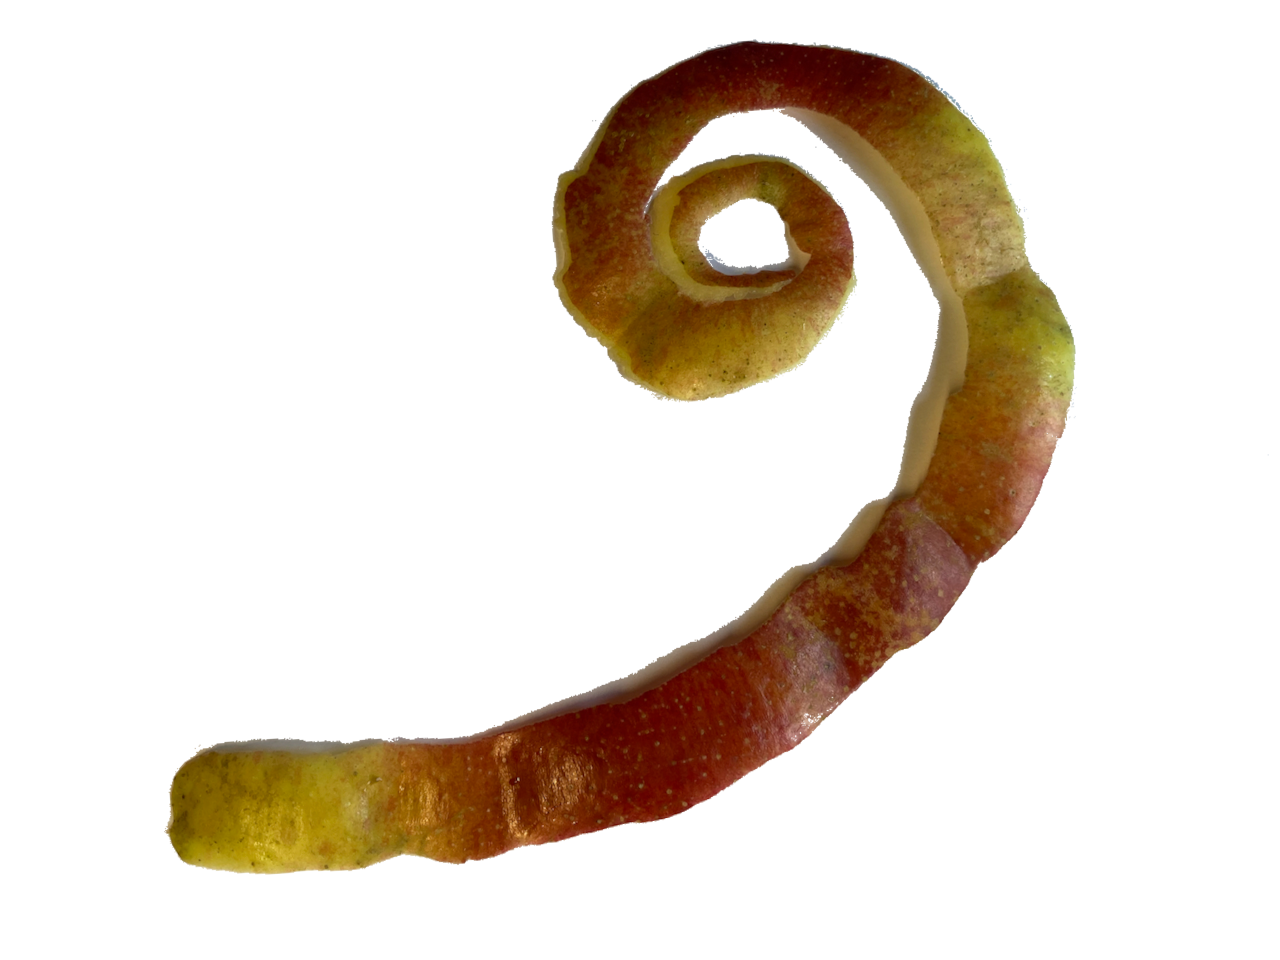
\includegraphics[width=9.4cm]{../slides/fresnel/apfel.png}};
}
\end{scope}
\draw[color=gray!50] (0,0) rectangle (4,4);
\draw[->] (-0.5,0) -- (7.5,0) coordinate[label={$C(t)$}];
\draw[->] (0,-0.5) -- (0,6.0) coordinate[label={left:$S(t)$}];
\uncover<3->{
\begin{scope}[scale=8]
\draw[color=red,opacity=0.5,line width=1.4pt] \fresnela;
\end{scope}
}
\end{tikzpicture}
\end{center}
\end{frame}
\egroup
